\setcounter{definition}{0} \setcounter{property}{0} \setcounter{claim}{0} \setcounter{fact}{0} \setcounter{corollary}{0} \setcounter{figure}{0}
\section{Connectivity of Directed Graphs}

\subsection*{Directed Acyclic Graphs}

Before we study the connectivity of directed graphs, we first
introduce a special class of directed graph, named directed acyclic graph~(DAG).

\begin{definition}[DAG]
A directed graph $G = (V, E)$ is \emph{acyclic} if and only if $G$ does not contain cycles.
\end{definition}

\begin{definition}[Linearization / Topological Sorting]
Let $G = (V,E)$ be a directed graph. Let $X$ be an ordering of $V$.
If $X$ satisfies: if $(v_i, v_j)\in E$, then $v_i$ is before $v_j$ in $X$,
then we say $X$ is a linearization~(or toplogical sorting) of $G$.
\end{definition}


See some examples below.

\begin{figure}[h!]
\centering{

\tikzset{every picture/.style={line width=0.75pt}} %set default line width to 0.75pt        

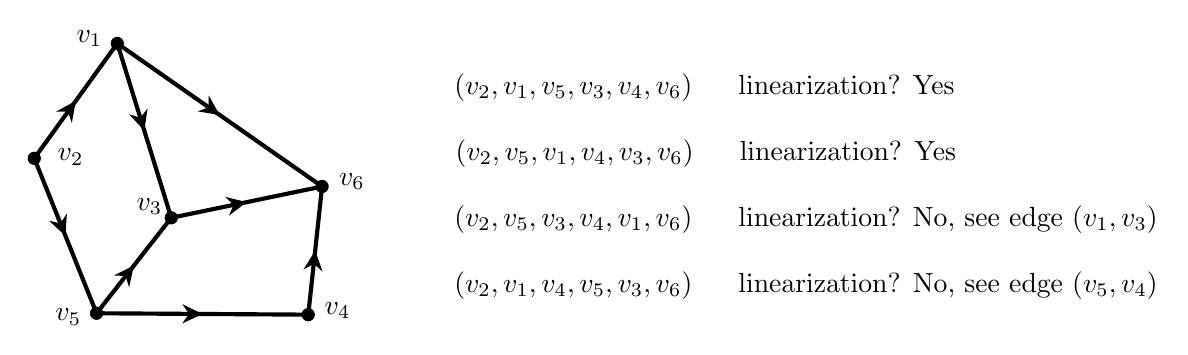
\begin{tikzpicture}[x=0.5pt,y=0.5pt,yscale=-1,xscale=1]
%uncomment if require: \path (0,228); %set diagram left start at 0, and has height of 228

%Flowchart: Connector [id:dp3072392280017706] 
\draw  [fill={rgb, 255:red, 0; green, 0; blue, 0 }  ,fill opacity=1 ] (78,14) .. controls (78,11.58) and (79.96,9.62) .. (82.38,9.62) .. controls (84.79,9.62) and (86.75,11.58) .. (86.75,14) .. controls (86.75,16.42) and (84.79,18.38) .. (82.38,18.38) .. controls (79.96,18.38) and (78,16.42) .. (78,14) -- cycle ;
%Flowchart: Connector [id:dp21397717392367266] 
\draw  [fill={rgb, 255:red, 0; green, 0; blue, 0 }  ,fill opacity=1 ] (63,209) .. controls (63,206.58) and (64.96,204.62) .. (67.38,204.62) .. controls (69.79,204.62) and (71.75,206.58) .. (71.75,209) .. controls (71.75,211.42) and (69.79,213.38) .. (67.38,213.38) .. controls (64.96,213.38) and (63,211.42) .. (63,209) -- cycle ;
%Flowchart: Connector [id:dp8067973087407497] 
\draw  [fill={rgb, 255:red, 0; green, 0; blue, 0 }  ,fill opacity=1 ] (18,97) .. controls (18,94.58) and (19.96,92.62) .. (22.38,92.62) .. controls (24.79,92.62) and (26.75,94.58) .. (26.75,97) .. controls (26.75,99.42) and (24.79,101.38) .. (22.38,101.38) .. controls (19.96,101.38) and (18,99.42) .. (18,97) -- cycle ;
%Flowchart: Connector [id:dp962987276172525] 
\draw  [fill={rgb, 255:red, 0; green, 0; blue, 0 }  ,fill opacity=1 ] (117,140) .. controls (117,137.58) and (118.96,135.62) .. (121.38,135.62) .. controls (123.79,135.62) and (125.75,137.58) .. (125.75,140) .. controls (125.75,142.42) and (123.79,144.38) .. (121.38,144.38) .. controls (118.96,144.38) and (117,142.42) .. (117,140) -- cycle ;
%Straight Lines [id:da5158988833498211] 
\draw [color={rgb, 255:red, 0; green, 0; blue, 0 }  ,draw opacity=1 ][line width=1.5]    (22.38,97) -- (82.38,14) ;
\draw [shift={(52.38,55.5)}, rotate = 125.86] [fill={rgb, 255:red, 0; green, 0; blue, 0 }  ,fill opacity=1 ][line width=0.08]  [draw opacity=0] (14.56,-6.99) -- (0,0) -- (14.56,6.99) -- (9.67,0) -- cycle    ;
%Straight Lines [id:da26521146489140124] 
\draw [color={rgb, 255:red, 0; green, 0; blue, 0 }  ,draw opacity=1 ][line width=1.5]    (67.38,209) -- (121.38,140) ;
\draw [shift={(94.38,174.5)}, rotate = 128.05] [fill={rgb, 255:red, 0; green, 0; blue, 0 }  ,fill opacity=1 ][line width=0.08]  [draw opacity=0] (14.56,-6.99) -- (0,0) -- (14.56,6.99) -- (9.67,0) -- cycle    ;
%Straight Lines [id:da2524996293078703] 
\draw [color={rgb, 255:red, 0; green, 0; blue, 0 }  ,draw opacity=1 ][line width=1.5]    (121.38,140) -- (82.38,14) ;
\draw [shift={(101.88,77)}, rotate = 252.8] [fill={rgb, 255:red, 0; green, 0; blue, 0 }  ,fill opacity=1 ][line width=0.08]  [draw opacity=0] (14.56,-6.99) -- (0,0) -- (14.56,6.99) -- (9.67,0) -- cycle    ;
%Straight Lines [id:da9962026070016303] 
\draw [color={rgb, 255:red, 0; green, 0; blue, 0 }  ,draw opacity=1 ][line width=1.5]    (67.38,209) -- (22.38,97) ;
\draw [shift={(44.88,153)}, rotate = 248.11] [fill={rgb, 255:red, 0; green, 0; blue, 0 }  ,fill opacity=1 ][line width=0.08]  [draw opacity=0] (14.56,-6.99) -- (0,0) -- (14.56,6.99) -- (9.67,0) -- cycle    ;
%Flowchart: Connector [id:dp1566790029206172] 
\draw  [fill={rgb, 255:red, 0; green, 0; blue, 0 }  ,fill opacity=1 ] (216,210) .. controls (216,207.58) and (217.96,205.62) .. (220.38,205.62) .. controls (222.79,205.62) and (224.75,207.58) .. (224.75,210) .. controls (224.75,212.42) and (222.79,214.38) .. (220.38,214.38) .. controls (217.96,214.38) and (216,212.42) .. (216,210) -- cycle ;
%Straight Lines [id:da5810218256695717] 
\draw [color={rgb, 255:red, 0; green, 0; blue, 0 }  ,draw opacity=1 ][line width=1.5]    (67.38,209) -- (220.38,210) ;
\draw [shift={(143.88,209.5)}, rotate = 180.37] [fill={rgb, 255:red, 0; green, 0; blue, 0 }  ,fill opacity=1 ][line width=0.08]  [draw opacity=0] (14.56,-6.99) -- (0,0) -- (14.56,6.99) -- (9.67,0) -- cycle    ;
%Flowchart: Connector [id:dp3466519048019897] 
\draw  [fill={rgb, 255:red, 0; green, 0; blue, 0 }  ,fill opacity=1 ] (226,117.38) .. controls (226,114.96) and (227.96,113) .. (230.38,113) .. controls (232.79,113) and (234.75,114.96) .. (234.75,117.38) .. controls (234.75,119.79) and (232.79,121.75) .. (230.38,121.75) .. controls (227.96,121.75) and (226,119.79) .. (226,117.38) -- cycle ;
%Straight Lines [id:da9047303683615766] 
\draw [color={rgb, 255:red, 0; green, 0; blue, 0 }  ,draw opacity=1 ][line width=1.5]    (121.38,140) -- (230.38,117.38) ;
\draw [shift={(175.88,128.69)}, rotate = 168.27] [fill={rgb, 255:red, 0; green, 0; blue, 0 }  ,fill opacity=1 ][line width=0.08]  [draw opacity=0] (14.56,-6.99) -- (0,0) -- (14.56,6.99) -- (9.67,0) -- cycle    ;
%Straight Lines [id:da5438432067917516] 
\draw [color={rgb, 255:red, 0; green, 0; blue, 0 }  ,draw opacity=1 ][line width=1.5]    (82.38,14) -- (230.38,117.38) ;
\draw [shift={(156.38,65.69)}, rotate = 214.93] [fill={rgb, 255:red, 0; green, 0; blue, 0 }  ,fill opacity=1 ][line width=0.08]  [draw opacity=0] (14.56,-6.99) -- (0,0) -- (14.56,6.99) -- (9.67,0) -- cycle    ;
%Straight Lines [id:da33002644345566856] 
\draw [color={rgb, 255:red, 0; green, 0; blue, 0 }  ,draw opacity=1 ][line width=1.5]    (220.38,210) -- (230.38,117.38) ;
\draw [shift={(225.38,163.69)}, rotate = 96.16] [fill={rgb, 255:red, 0; green, 0; blue, 0 }  ,fill opacity=1 ][line width=0.08]  [draw opacity=0] (14.56,-6.99) -- (0,0) -- (14.56,6.99) -- (9.67,0) -- cycle    ;

% Text Node
\draw (51,3) node [anchor=north west][inner sep=0.75pt]   [align=left] {$\displaystyle v_{1}$};
% Text Node
\draw (94.38,124.38) node [anchor=north west][inner sep=0.75pt]   [align=left] {$\displaystyle v_{3}$};
% Text Node
\draw (35.75,204) node [anchor=north west][inner sep=0.75pt]   [align=left] {$\displaystyle v_{5}$};
% Text Node
\draw (230.38,199.38) node [anchor=north west][inner sep=0.75pt]   [align=left] {$\displaystyle v_{4}$};
% Text Node
\draw (37.38,88.38) node [anchor=north west][inner sep=0.75pt]   [align=left] {$\displaystyle v_{2}$};
% Text Node
\draw (240.75,106.35) node [anchor=north west][inner sep=0.75pt]   [align=left] {$\displaystyle v_{6}$};
% Text Node
\draw (324,34) node [anchor=north west][inner sep=0.75pt]   [align=left] {$\displaystyle ( v_{2} ,v_{1} ,v_{5} ,v_{3} ,v_{4} ,v_{6})$ \ \ \ \ linearization? Yes};
% Text Node
\draw (325,81.67) node [anchor=north west][inner sep=0.75pt]   [align=left] {$\displaystyle ( v_{2} ,v_{5} ,v_{1} ,v_{4} ,v_{3} ,v_{6})$ \ \ \ \ linearization? Yes};
% Text Node
\draw (324,129.34) node [anchor=north west][inner sep=0.75pt]   [align=left] {$\displaystyle ( v_{2} ,v_{5} ,v_{3} ,v_{4} ,v_{1} ,v_{6})$ \ \ \ \ linearization? No, see edge $\displaystyle ( v_{1} ,v_{3})$};
% Text Node
\draw (324,177) node [anchor=north west][inner sep=0.75pt]   [align=left] {$\displaystyle ( v_{2} ,v_{1} ,v_{4} ,v_{5} ,v_{3} ,v_{6})$ \ \ \ \ linearization? No, see edge $\displaystyle ( v_{5} ,v_{4})$};


\end{tikzpicture}

}
\caption{Examples of linearization.}
\end{figure}

If a directed graph $G$ admits a linearization, then we say $G$ can be \emph{linearized}.
We now show that linearization is an \emph{equivalent} characterization of DAGs.

\begin{claim}
A directed graph $G$ can be linearized if and only if $G$ is a DAG.
\label{claim:dag}
\end{claim}

\emph{Proof.}  Let's first prove that if $G$ can be linearized, then $G$ is a DAG.
This is equivalent to proving its contraposition: if $G$ contains a cycle, then $G$ cannot be linearized.
Suppose that there exists an cycle $v_{i_1} \to v_{i_2} \to \cdots \to v_{i_k} \to v_{i_1}$ in $G$.
Then the linearization $X$ must satisfy that $v_{i_{j}}$ is before $v_{i_{j+1}}$ for all $j = 1, 2, \cdots, k-1$,
and that $v_{i_{k}}$ is before $v_{i_1}$, in $X$. Clearly, this is not possible.

The other side of the statement, i.e., if $G$ is a DAG, then $G$ can always be linearized, can be proved constructively.
We will design an algorithm~(see below), that constructs a linearization for any DAG. \qed


Let $G = (V, E)$ be a directed graph. 
If a vertex $v\in V$ does not have any in-edges~(i.e., \emph{in-degree} is 0), we call it \emph{source vertex};
if a vertex $v\in V$ does not have any out-edges~(i.e., \emph{out-degree} is 0), we call it \emph{sink vertex}.

A directed graph may contain multiple source vertices or sink vertices,
or may not have any source vertex or sink vertex. (Can you give such examples?)

\begin{claim}
A DAG $G=(V,E)$ always has source vertex and sink vertex.
\end{claim}
\emph{Proof.} Let's prove it by contradiction. Assume that $G$ does not contain any source.
First, $G$ must not contain self-loop as otherwise $G$ won't be a DAG.
Let $v$ be any vertex in $V$. As $v$ is not a source, we know that there exists some vertex $u$ points to $v$, i.e., $(u,v)\in E$.
Now since $u$ is not a source then there must exist another vertex $w$ such that $(w,u)\in E$.
Notice that $w \neq v$ as otherwise there will be a cycle: $v = w \to u \to v$.
This means that $w$ is a new vertex. Again as $w$ is not a source, there must exist another \emph{new} vertex points to it.
This process can be extended infinitely following the fact and assumption that $G$ is a DAG and all vertices not are sources,
but this is not possible as the number of vertices is limited. 
The existence of sink can be proved symmetrically. \qed


Following above fact, we can design an algorithm to find a linearization of a DAG: it iteratively
finds source vertex and removes it and its adjacent edges.

\begin{minipage}{0.8\textwidth}
	\aaA {7}{Algorithm find-linearization ($G = (V, E)$)}\xxx
	\aab {init $X$ as empty list;}\xxx
	\aaB {4}{while ($|X| < |V|$)}\xxx
	\aac {arbitrarily find a source vertex $u$ of $G$;}\xxx
	\aac {add $u$ to the end of $X$;}\xxx
	\aac {remove $u$ and its adjacent edges;}\xxx
	\aab {end while;}\xxx
	\aaa {end algorithm;}\xxx
\end{minipage}

This algorithm is correct. First, when a vertex $u$ is added to $X$,
it is a source vertex of the current graph, which means that
$\{w\mid (w, u)\in E\}$ is either empty or all of them
have been added to $X$. Second, $X$ will include all vertices.
This is because, a source always exists in a DAG~(as we just proved).
The above algorithm is more a framework, as how we update the graph
is not given specifically, and which affects the running time.

Above algorithm also gives a constructive proof that, a DAG can always
be linearized. This completes the proof stated in previous lecture: a directed graph is a DAG if and only if it can be linearized.

\begin{claim}
Let $X$ be any linearization of a DAG. Then the first vertex of $X$ is a source vertex and 
the last vertex of of $X$ is a sink vertex.
\label{claim:source}
\end{claim}

\emph{Proof.} Let $v_1$ be the first vertex of $X$. Suppose that $v_1$ is not a source of $X$. 
By definition of (not being a) source vertex, there exists $(u,v_1)\in E$. Then by the definition
of linearization, we know that $u$ will be before $v_1$ in $X$, contradicting to the fact that
$v_1$ is the first element of $X$.
The other side can be proved symmetrically. \qed

We can use above algorithm to constructively prove following statement.

\begin{claim}
Let $G = (V, E)$ be a DAG. A vertex $u\in V$ is a source if and only if 
there exists a linearization $X$ of $G$ such that $u$ is the first vertex in $X$.
\end{claim}

\emph{Proof.} We first prove that, if $u$ is a source, then there exists a linearization
where $u$ is the first vertex of $X$. We prove it by showing that,
we can construct such a linearization $X$. We can use above algorithm,
and in its first step, we simply pick $u$. The correctness of above algorithm
explains the rest.  The other side is exactly Claim~\ref{claim:source}, which we have proved. \qed


\subsection*{Meta-Graph}

For a directed graph $G = (V,E)$, its structure of connectivity can be represented as a new
directed graph, called \emph{meta-graph}, denoted as $G_M = (V_M, E_M)$.
Each of the vertices of the meta-graph corresponds to a connected component of $G$,
and two vertices $C_i, C_j  \in V_M$ are connected by edge $(C_i, C_j) \in E_M$
if and only if there exists edge $(u,v)\in E$ such that $u\in C_i$ and $v\in C_j$.
An example of meta-graph is given below.

\begin{figure}[h!]
\centering{

\tikzset{every picture/.style={line width=0.75pt}} %set default line width to 0.75pt        

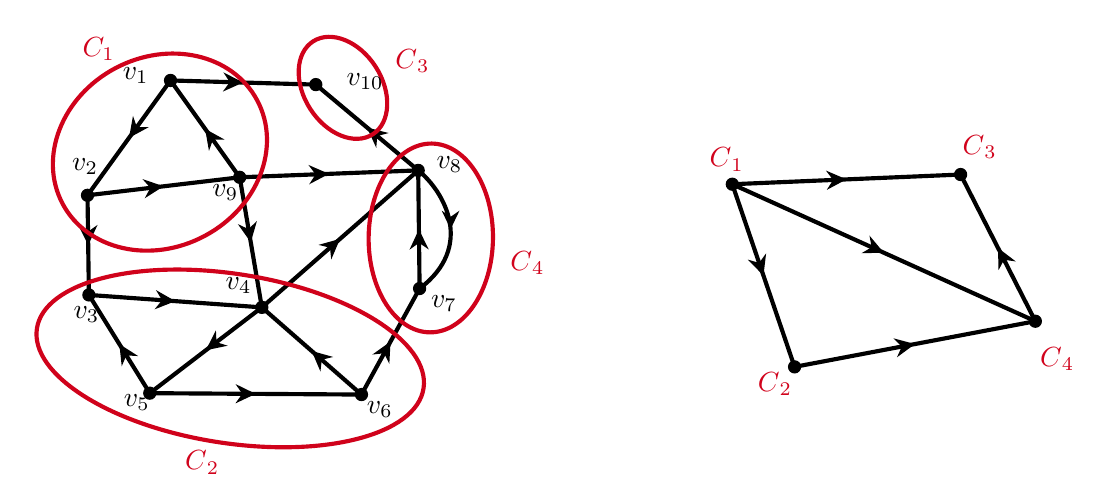
\begin{tikzpicture}[x=0.5pt,y=0.5pt,yscale=-1,xscale=1]
%uncomment if require: \path (0,510); %set diagram left start at 0, and has height of 510

%Flowchart: Connector [id:dp5937668531638635] 
\draw  [fill={rgb, 255:red, 0; green, 0; blue, 0 }  ,fill opacity=1 ] (139,106) .. controls (139,103.58) and (140.96,101.62) .. (143.38,101.62) .. controls (145.79,101.62) and (147.75,103.58) .. (147.75,106) .. controls (147.75,108.42) and (145.79,110.38) .. (143.38,110.38) .. controls (140.96,110.38) and (139,108.42) .. (139,106) -- cycle ;
%Flowchart: Connector [id:dp6657935561963445] 
\draw  [fill={rgb, 255:red, 0; green, 0; blue, 0 }  ,fill opacity=1 ] (244,109) .. controls (244,106.58) and (245.96,104.62) .. (248.38,104.62) .. controls (250.79,104.62) and (252.75,106.58) .. (252.75,109) .. controls (252.75,111.42) and (250.79,113.38) .. (248.38,113.38) .. controls (245.96,113.38) and (244,111.42) .. (244,109) -- cycle ;
%Flowchart: Connector [id:dp14354113795738999] 
\draw  [fill={rgb, 255:red, 0; green, 0; blue, 0 }  ,fill opacity=1 ] (124,332) .. controls (124,329.58) and (125.96,327.62) .. (128.38,327.62) .. controls (130.79,327.62) and (132.75,329.58) .. (132.75,332) .. controls (132.75,334.42) and (130.79,336.38) .. (128.38,336.38) .. controls (125.96,336.38) and (124,334.42) .. (124,332) -- cycle ;
%Flowchart: Connector [id:dp3081556962622095] 
\draw  [fill={rgb, 255:red, 0; green, 0; blue, 0 }  ,fill opacity=1 ] (79,189) .. controls (79,186.58) and (80.96,184.62) .. (83.38,184.62) .. controls (85.79,184.62) and (87.75,186.58) .. (87.75,189) .. controls (87.75,191.42) and (85.79,193.38) .. (83.38,193.38) .. controls (80.96,193.38) and (79,191.42) .. (79,189) -- cycle ;
%Flowchart: Connector [id:dp20013554043379078] 
\draw  [fill={rgb, 255:red, 0; green, 0; blue, 0 }  ,fill opacity=1 ] (189,176) .. controls (189,173.58) and (190.96,171.62) .. (193.38,171.62) .. controls (195.79,171.62) and (197.75,173.58) .. (197.75,176) .. controls (197.75,178.42) and (195.79,180.38) .. (193.38,180.38) .. controls (190.96,180.38) and (189,178.42) .. (189,176) -- cycle ;
%Straight Lines [id:da8865551056781525] 
\draw [color={rgb, 255:red, 0; green, 0; blue, 0 }  ,draw opacity=1 ][line width=1.5]    (83.38,189) -- (143.38,106) ;
\draw [shift={(113.38,147.5)}, rotate = 305.86] [fill={rgb, 255:red, 0; green, 0; blue, 0 }  ,fill opacity=1 ][line width=0.08]  [draw opacity=0] (14.56,-6.99) -- (0,0) -- (14.56,6.99) -- (9.67,0) -- cycle    ;
%Straight Lines [id:da4408247919919335] 
\draw [color={rgb, 255:red, 0; green, 0; blue, 0 }  ,draw opacity=1 ][line width=1.5]    (128.38,332) -- (209.38,270) ;
\draw [shift={(168.88,301)}, rotate = 322.57] [fill={rgb, 255:red, 0; green, 0; blue, 0 }  ,fill opacity=1 ][line width=0.08]  [draw opacity=0] (14.56,-6.99) -- (0,0) -- (14.56,6.99) -- (9.67,0) -- cycle    ;
%Straight Lines [id:da8012008000621113] 
\draw [color={rgb, 255:red, 0; green, 0; blue, 0 }  ,draw opacity=1 ][line width=1.5]    (193.38,176) -- (83.38,189) ;
\draw [shift={(138.38,182.5)}, rotate = 173.26] [fill={rgb, 255:red, 0; green, 0; blue, 0 }  ,fill opacity=1 ][line width=0.08]  [draw opacity=0] (14.56,-6.99) -- (0,0) -- (14.56,6.99) -- (9.67,0) -- cycle    ;
%Straight Lines [id:da01269837290493725] 
\draw [color={rgb, 255:red, 0; green, 0; blue, 0 }  ,draw opacity=1 ][line width=1.5]    (128.38,332) -- (84.38,261) ;
\draw [shift={(106.38,296.5)}, rotate = 418.21000000000004] [fill={rgb, 255:red, 0; green, 0; blue, 0 }  ,fill opacity=1 ][line width=0.08]  [draw opacity=0] (14.56,-6.99) -- (0,0) -- (14.56,6.99) -- (9.67,0) -- cycle    ;
%Flowchart: Connector [id:dp01738972677326256] 
\draw  [fill={rgb, 255:red, 0; green, 0; blue, 0 }  ,fill opacity=1 ] (277,333) .. controls (277,330.58) and (278.96,328.62) .. (281.38,328.62) .. controls (283.79,328.62) and (285.75,330.58) .. (285.75,333) .. controls (285.75,335.42) and (283.79,337.38) .. (281.38,337.38) .. controls (278.96,337.38) and (277,335.42) .. (277,333) -- cycle ;
%Straight Lines [id:da9151099863353562] 
\draw [color={rgb, 255:red, 0; green, 0; blue, 0 }  ,draw opacity=1 ][line width=1.5]    (281.38,333) -- (323.38,256.38) ;
\draw [shift={(302.38,294.69)}, rotate = 478.73] [fill={rgb, 255:red, 0; green, 0; blue, 0 }  ,fill opacity=1 ][line width=0.08]  [draw opacity=0] (14.56,-6.99) -- (0,0) -- (14.56,6.99) -- (9.67,0) -- cycle    ;
%Straight Lines [id:da8589700496158776] 
\draw [color={rgb, 255:red, 0; green, 0; blue, 0 }  ,draw opacity=1 ][line width=1.5]    (128.38,332) -- (281.38,333) ;
\draw [shift={(204.88,332.5)}, rotate = 180.37] [fill={rgb, 255:red, 0; green, 0; blue, 0 }  ,fill opacity=1 ][line width=0.08]  [draw opacity=0] (14.56,-6.99) -- (0,0) -- (14.56,6.99) -- (9.67,0) -- cycle    ;
%Flowchart: Connector [id:dp23564521467293476] 
\draw  [fill={rgb, 255:red, 0; green, 0; blue, 0 }  ,fill opacity=1 ] (319,256.38) .. controls (319,253.96) and (320.96,252) .. (323.38,252) .. controls (325.79,252) and (327.75,253.96) .. (327.75,256.38) .. controls (327.75,258.79) and (325.79,260.75) .. (323.38,260.75) .. controls (320.96,260.75) and (319,258.79) .. (319,256.38) -- cycle ;
%Straight Lines [id:da5765902383361479] 
\draw [color={rgb, 255:red, 0; green, 0; blue, 0 }  ,draw opacity=1 ][line width=1.5]    (323.38,256.38) -- (322.38,171) ;
\draw [shift={(322.88,213.69)}, rotate = 449.33] [fill={rgb, 255:red, 0; green, 0; blue, 0 }  ,fill opacity=1 ][line width=0.08]  [draw opacity=0] (14.56,-6.99) -- (0,0) -- (14.56,6.99) -- (9.67,0) -- cycle    ;
%Straight Lines [id:da6859280233883376] 
\draw [color={rgb, 255:red, 0; green, 0; blue, 0 }  ,draw opacity=1 ][line width=1.5]    (322.38,171) -- (248.38,109) ;
\draw [shift={(285.38,140)}, rotate = 399.96000000000004] [fill={rgb, 255:red, 0; green, 0; blue, 0 }  ,fill opacity=1 ][line width=0.08]  [draw opacity=0] (14.56,-6.99) -- (0,0) -- (14.56,6.99) -- (9.67,0) -- cycle    ;
%Straight Lines [id:da329141247373788] 
\draw [color={rgb, 255:red, 0; green, 0; blue, 0 }  ,draw opacity=1 ][line width=1.5]    (143.38,106) -- (193.38,176) ;
\draw [shift={(168.38,141)}, rotate = 54.46] [fill={rgb, 255:red, 0; green, 0; blue, 0 }  ,fill opacity=1 ][line width=0.08]  [draw opacity=0] (14.56,-6.99) -- (0,0) -- (14.56,6.99) -- (9.67,0) -- cycle    ;
%Straight Lines [id:da25009890870323437] 
\draw [color={rgb, 255:red, 0; green, 0; blue, 0 }  ,draw opacity=1 ][line width=1.5]    (209.38,270) -- (281.38,333) ;
\draw [shift={(245.38,301.5)}, rotate = 41.19] [fill={rgb, 255:red, 0; green, 0; blue, 0 }  ,fill opacity=1 ][line width=0.08]  [draw opacity=0] (14.56,-6.99) -- (0,0) -- (14.56,6.99) -- (9.67,0) -- cycle    ;
%Flowchart: Connector [id:dp20561620581532858] 
\draw  [fill={rgb, 255:red, 0; green, 0; blue, 0 }  ,fill opacity=1 ] (205,270) .. controls (205,267.58) and (206.96,265.62) .. (209.38,265.62) .. controls (211.79,265.62) and (213.75,267.58) .. (213.75,270) .. controls (213.75,272.42) and (211.79,274.38) .. (209.38,274.38) .. controls (206.96,274.38) and (205,272.42) .. (205,270) -- cycle ;
%Flowchart: Connector [id:dp4014605163661533] 
\draw  [fill={rgb, 255:red, 0; green, 0; blue, 0 }  ,fill opacity=1 ] (80,261) .. controls (80,258.58) and (81.96,256.62) .. (84.38,256.62) .. controls (86.79,256.62) and (88.75,258.58) .. (88.75,261) .. controls (88.75,263.42) and (86.79,265.38) .. (84.38,265.38) .. controls (81.96,265.38) and (80,263.42) .. (80,261) -- cycle ;
%Flowchart: Connector [id:dp14845565107772662] 
\draw  [fill={rgb, 255:red, 0; green, 0; blue, 0 }  ,fill opacity=1 ] (318,171) .. controls (318,168.58) and (319.96,166.62) .. (322.38,166.62) .. controls (324.79,166.62) and (326.75,168.58) .. (326.75,171) .. controls (326.75,173.42) and (324.79,175.38) .. (322.38,175.38) .. controls (319.96,175.38) and (318,173.42) .. (318,171) -- cycle ;
%Straight Lines [id:da3881378688310262] 
\draw [color={rgb, 255:red, 0; green, 0; blue, 0 }  ,draw opacity=1 ][line width=1.5]    (209.38,270) -- (84.38,261) ;
\draw [shift={(146.88,265.5)}, rotate = 184.12] [fill={rgb, 255:red, 0; green, 0; blue, 0 }  ,fill opacity=1 ][line width=0.08]  [draw opacity=0] (14.56,-6.99) -- (0,0) -- (14.56,6.99) -- (9.67,0) -- cycle    ;
%Curve Lines [id:da8015709651805362] 
\draw [line width=1.5]    (323.38,256.38) .. controls (363.38,226.38) and (341.68,186.52) .. (322.38,171) ;
\draw [shift={(345.77,213.48)}, rotate = 270.05] [fill={rgb, 255:red, 0; green, 0; blue, 0 }  ][line width=0.08]  [draw opacity=0] (13.4,-6.43) -- (0,0) -- (13.4,6.44) -- (8.9,0) -- cycle    ;
%Straight Lines [id:da4386825484478063] 
\draw [color={rgb, 255:red, 0; green, 0; blue, 0 }  ,draw opacity=1 ][line width=1.5]    (209.38,270) -- (322.38,171) ;
\draw [shift={(265.88,220.5)}, rotate = 498.78] [fill={rgb, 255:red, 0; green, 0; blue, 0 }  ,fill opacity=1 ][line width=0.08]  [draw opacity=0] (14.56,-6.99) -- (0,0) -- (14.56,6.99) -- (9.67,0) -- cycle    ;
%Straight Lines [id:da26616639892534444] 
\draw [color={rgb, 255:red, 0; green, 0; blue, 0 }  ,draw opacity=1 ][line width=1.5]    (193.38,176) -- (209.38,270) ;
\draw [shift={(201.38,223)}, rotate = 260.34000000000003] [fill={rgb, 255:red, 0; green, 0; blue, 0 }  ,fill opacity=1 ][line width=0.08]  [draw opacity=0] (14.56,-6.99) -- (0,0) -- (14.56,6.99) -- (9.67,0) -- cycle    ;
%Straight Lines [id:da34500416847135773] 
\draw [color={rgb, 255:red, 0; green, 0; blue, 0 }  ,draw opacity=1 ][line width=1.5]    (83.38,189) -- (84.38,261) ;
\draw [shift={(83.88,225)}, rotate = 269.2] [fill={rgb, 255:red, 0; green, 0; blue, 0 }  ,fill opacity=1 ][line width=0.08]  [draw opacity=0] (14.56,-6.99) -- (0,0) -- (14.56,6.99) -- (9.67,0) -- cycle    ;
%Straight Lines [id:da4267721016610234] 
\draw [color={rgb, 255:red, 0; green, 0; blue, 0 }  ,draw opacity=1 ][line width=1.5]    (193.38,176) -- (322.38,171) ;
\draw [shift={(257.88,173.5)}, rotate = 537.78] [fill={rgb, 255:red, 0; green, 0; blue, 0 }  ,fill opacity=1 ][line width=0.08]  [draw opacity=0] (14.56,-6.99) -- (0,0) -- (14.56,6.99) -- (9.67,0) -- cycle    ;
%Straight Lines [id:da8164594223234878] 
\draw [color={rgb, 255:red, 0; green, 0; blue, 0 }  ,draw opacity=1 ][line width=1.5]    (143.38,106) -- (248.38,109) ;
\draw [shift={(195.88,107.5)}, rotate = 181.64] [fill={rgb, 255:red, 0; green, 0; blue, 0 }  ,fill opacity=1 ][line width=0.08]  [draw opacity=0] (14.56,-6.99) -- (0,0) -- (14.56,6.99) -- (9.67,0) -- cycle    ;
%Shape: Ellipse [id:dp27109176732345586] 
\draw  [color={rgb, 255:red, 208; green, 2; blue, 27 }  ,draw opacity=1 ][line width=1.5]  (65.39,195.12) .. controls (47.61,161.62) and (64.68,117.75) .. (103.52,97.13) .. controls (142.37,76.52) and (188.27,86.96) .. (206.05,120.45) .. controls (223.83,153.95) and (206.76,197.82) .. (167.91,218.44) .. controls (129.07,239.06) and (83.17,228.61) .. (65.39,195.12) -- cycle ;
%Shape: Ellipse [id:dp0877469193537469] 
\draw  [color={rgb, 255:red, 208; green, 2; blue, 27 }  ,draw opacity=1 ][line width=1.5]  (46.82,285.18) .. controls (52.01,251.81) and (118.75,234.47) .. (195.91,246.46) .. controls (273.06,258.44) and (331.4,295.21) .. (326.22,328.58) .. controls (321.04,361.95) and (254.29,379.29) .. (177.14,367.3) .. controls (99.98,355.32) and (41.64,318.55) .. (46.82,285.18) -- cycle ;
%Shape: Ellipse [id:dp6318272598845582] 
\draw  [color={rgb, 255:red, 208; green, 2; blue, 27 }  ,draw opacity=1 ][line width=1.5]  (332.2,151.61) .. controls (357.02,151.88) and (376.8,182.63) .. (376.4,220.31) .. controls (376,257.98) and (355.56,288.31) .. (330.75,288.04) .. controls (305.94,287.78) and (286.15,257.02) .. (286.55,219.35) .. controls (286.96,181.68) and (307.39,151.35) .. (332.2,151.61) -- cycle ;
%Shape: Ellipse [id:dp1869855316402914] 
\draw  [color={rgb, 255:red, 208; green, 2; blue, 27 }  ,draw opacity=1 ][line width=1.5]  (246.45,77.74) .. controls (259.53,69.36) and (279.77,77.6) .. (291.66,96.15) .. controls (303.55,114.71) and (302.58,136.54) .. (289.5,144.92) .. controls (276.42,153.3) and (256.19,145.05) .. (244.3,126.5) .. controls (232.41,107.95) and (233.38,86.12) .. (246.45,77.74) -- cycle ;
%Flowchart: Connector [id:dp51888588365958] 
\draw  [fill={rgb, 255:red, 0; green, 0; blue, 0 }  ,fill opacity=1 ] (590,313) .. controls (590,310.58) and (591.96,308.62) .. (594.38,308.62) .. controls (596.79,308.62) and (598.75,310.58) .. (598.75,313) .. controls (598.75,315.42) and (596.79,317.38) .. (594.38,317.38) .. controls (591.96,317.38) and (590,315.42) .. (590,313) -- cycle ;
%Straight Lines [id:da6410921260405182] 
\draw [color={rgb, 255:red, 0; green, 0; blue, 0 }  ,draw opacity=1 ][line width=1.5]    (768.38,280) -- (549.38,181) ;
\draw [shift={(658.88,230.5)}, rotate = 204.33] [fill={rgb, 255:red, 0; green, 0; blue, 0 }  ,fill opacity=1 ][line width=0.08]  [draw opacity=0] (14.56,-6.99) -- (0,0) -- (14.56,6.99) -- (9.67,0) -- cycle    ;
%Straight Lines [id:da8627356399127929] 
\draw [color={rgb, 255:red, 0; green, 0; blue, 0 }  ,draw opacity=1 ][line width=1.5]    (768.38,280) -- (714.38,174) ;
\draw [shift={(741.38,227)}, rotate = 423] [fill={rgb, 255:red, 0; green, 0; blue, 0 }  ,fill opacity=1 ][line width=0.08]  [draw opacity=0] (14.56,-6.99) -- (0,0) -- (14.56,6.99) -- (9.67,0) -- cycle    ;
%Flowchart: Connector [id:dp5660576336850748] 
\draw  [fill={rgb, 255:red, 0; green, 0; blue, 0 }  ,fill opacity=1 ] (710,174) .. controls (710,171.58) and (711.96,169.62) .. (714.38,169.62) .. controls (716.79,169.62) and (718.75,171.58) .. (718.75,174) .. controls (718.75,176.42) and (716.79,178.38) .. (714.38,178.38) .. controls (711.96,178.38) and (710,176.42) .. (710,174) -- cycle ;
%Flowchart: Connector [id:dp5784688617216504] 
\draw  [fill={rgb, 255:red, 0; green, 0; blue, 0 }  ,fill opacity=1 ] (545,181) .. controls (545,178.58) and (546.96,176.62) .. (549.38,176.62) .. controls (551.79,176.62) and (553.75,178.58) .. (553.75,181) .. controls (553.75,183.42) and (551.79,185.38) .. (549.38,185.38) .. controls (546.96,185.38) and (545,183.42) .. (545,181) -- cycle ;
%Straight Lines [id:da35390930720516367] 
\draw [color={rgb, 255:red, 0; green, 0; blue, 0 }  ,draw opacity=1 ][line width=1.5]    (594.38,313) -- (549.38,181) ;
\draw [shift={(571.88,247)}, rotate = 251.18] [fill={rgb, 255:red, 0; green, 0; blue, 0 }  ,fill opacity=1 ][line width=0.08]  [draw opacity=0] (14.56,-6.99) -- (0,0) -- (14.56,6.99) -- (9.67,0) -- cycle    ;
%Straight Lines [id:da16486738526478106] 
\draw [color={rgb, 255:red, 0; green, 0; blue, 0 }  ,draw opacity=1 ][line width=1.5]    (549.38,181) -- (714.38,174) ;
\draw [shift={(631.88,177.5)}, rotate = 537.5699999999999] [fill={rgb, 255:red, 0; green, 0; blue, 0 }  ,fill opacity=1 ][line width=0.08]  [draw opacity=0] (14.56,-6.99) -- (0,0) -- (14.56,6.99) -- (9.67,0) -- cycle    ;
%Flowchart: Connector [id:dp49963370359380055] 
\draw  [fill={rgb, 255:red, 0; green, 0; blue, 0 }  ,fill opacity=1 ] (764,280) .. controls (764,277.58) and (765.96,275.62) .. (768.38,275.62) .. controls (770.79,275.62) and (772.75,277.58) .. (772.75,280) .. controls (772.75,282.42) and (770.79,284.38) .. (768.38,284.38) .. controls (765.96,284.38) and (764,282.42) .. (764,280) -- cycle ;
%Straight Lines [id:da8408093021248022] 
\draw [color={rgb, 255:red, 0; green, 0; blue, 0 }  ,draw opacity=1 ][line width=1.5]    (768.38,280) -- (594.38,313) ;
\draw [shift={(681.38,296.5)}, rotate = 169.26] [fill={rgb, 255:red, 0; green, 0; blue, 0 }  ,fill opacity=1 ][line width=0.08]  [draw opacity=0] (14.56,-6.99) -- (0,0) -- (14.56,6.99) -- (9.67,0) -- cycle    ;

% Text Node
\draw (107,94.93) node [anchor=north west][inner sep=0.75pt]   [align=left] {$\displaystyle v_{1}$};
% Text Node
\draw (71.38,267.31) node [anchor=north west][inner sep=0.75pt]   [align=left] {$\displaystyle v_{3}$};
% Text Node
\draw (107.75,330.93) node [anchor=north west][inner sep=0.75pt]   [align=left] {$\displaystyle v_{5}$};
% Text Node
\draw (181.38,246.31) node [anchor=north west][inner sep=0.75pt]   [align=left] {$\displaystyle v_{4}$};
% Text Node
\draw (70.38,160.31) node [anchor=north west][inner sep=0.75pt]   [align=left] {$\displaystyle v_{2}$};
% Text Node
\draw (171.75,179.29) node [anchor=north west][inner sep=0.75pt]   [align=left] {$\displaystyle v_{9}$};
% Text Node
\draw (329.75,259.31) node [anchor=north west][inner sep=0.75pt]   [align=left] {$\displaystyle v_{7}$};
% Text Node
\draw (283.38,335.93) node [anchor=north west][inner sep=0.75pt]   [align=left] {$\displaystyle v_{6}$};
% Text Node
\draw (333.75,159.29) node [anchor=north west][inner sep=0.75pt]   [align=left] {$\displaystyle v_{8}$};
% Text Node
\draw (268.75,99.29) node [anchor=north west][inner sep=0.75pt]   [align=left] {$\displaystyle v_{10}$};
% Text Node
\draw (78,72.93) node [anchor=north west][inner sep=0.75pt]   [align=left] {$\displaystyle \textcolor[rgb]{0.82,0.01,0.11}{C_{1}}$};
% Text Node
\draw (152,371.93) node [anchor=north west][inner sep=0.75pt]   [align=left] {$\displaystyle \textcolor[rgb]{0.82,0.01,0.11}{C}\textcolor[rgb]{0.82,0.01,0.11}{_{2}}$};
% Text Node
\draw (387,227.93) node [anchor=north west][inner sep=0.75pt]   [align=left] {$\displaystyle \textcolor[rgb]{0.82,0.01,0.11}{C}\textcolor[rgb]{0.82,0.01,0.11}{_{4}}$};
% Text Node
\draw (304,81.93) node [anchor=north west][inner sep=0.75pt]   [align=left] {$\displaystyle \textcolor[rgb]{0.82,0.01,0.11}{C}\textcolor[rgb]{0.82,0.01,0.11}{_{3}}$};
% Text Node
\draw (566,314.93) node [anchor=north west][inner sep=0.75pt]   [align=left] {$\displaystyle \textcolor[rgb]{0.82,0.01,0.11}{C}\textcolor[rgb]{0.82,0.01,0.11}{_{2}}$};
% Text Node
\draw (770,296.93) node [anchor=north west][inner sep=0.75pt]   [align=left] {$\displaystyle \textcolor[rgb]{0.82,0.01,0.11}{C}\textcolor[rgb]{0.82,0.01,0.11}{_{4}}$};
% Text Node
\draw (531,152.93) node [anchor=north west][inner sep=0.75pt]   [align=left] {$\displaystyle \textcolor[rgb]{0.82,0.01,0.11}{C}\textcolor[rgb]{0.82,0.01,0.11}{_{1}}$};
% Text Node
\draw (714,143.93) node [anchor=north west][inner sep=0.75pt]   [align=left] {$\displaystyle \textcolor[rgb]{0.82,0.01,0.11}{C}\textcolor[rgb]{0.82,0.01,0.11}{_{3}}$};


\end{tikzpicture}

}
\caption{Example of meta-graph.}
\label{fig:meta-graph}
\end{figure}

Meta-graph has an important property: it does not contain cycles, i.e., it is a directed acyclic graph~(DAG).

\begin{claim}
The meta-graph $G_M$ of any directed graph $G$ is a directed acyclic graph.
\end{claim}

\emph{Proof.} Suppose conversely that $G_M$ contains a cycle, $C_1 \to C_2 \to C_k \to C_1$,
then the union of the vertices in these connected components form a single connected component,
contradicting to the \emph{maximal} property of connected component. \qed

We now design algorithms to determine the connected components of directed graphs and then to construct
the corresponding meta-graph.
Recall that the DFS algorithm introduced in Lecture A9 can successfully determine all connected components in an undirected graph.
Does this work also work for directed graph? Let's try. See Figure~\ref{fig:dfs-meta}.
Recall that the (top-layer) of the DFS algorithm is to tranverse all vertices in some ordering,
and if the current vertex $v$ is not yet visited, we will explore $v$.
For the example in Figure~\ref{fig:dfs-meta}, let's try it with the (natrual) ordering $v_1, v_2, \cdots, v_{10}$.
The resulting visited array is given in the figure~(please make sure you try it yourself).
Unfortunately, it does not give all connected components. In fact, the vertices marked as ``1''s are the union of $C_3$ and $C_4$,
and the vertices marked as ``2''s are the union of $C_1$ and $C_2$.
The reason is quite clear: we start with explore $v_1$, and during it all vertices reachable from $v_1$ will be marked as ``1'' in the visted array.
It turns out that $v_1$ is in connected component $C_4$, and $C_4$ can reach $C_3$ in the meta-graph.
Therefore, all vertices in $C_4$ and $C_3$ are reachable from $v_1$; consequently, the visited array is set as ``1'' for 
vertices in $C_4$ and $C_3$ during explore $v_1$. 
Similarly, we can also see why the vertices marked as ``2''s are the union of $C_1$ and $C_2$.
After exploring $v_1$, $\{v_1,v_2,v_7\}$ are visited; the next unvisited vertex is $v_3$ according to above natural ordering,
the the algorithm will explore $v_3$.
Again, during it all (unvisited) vertices reachable from $v_3$ will be marked as ``2'' in the visted array.
It turns out that $v_3$ is in connected component $C_1$, and $C_1$ can reach $C_2$ in the meta-graph.
Therefore, all vertices in $C_1$ and $C_2$ are reachable from $v_2$;
consequently, the visited array is set as ``2'' for 
vertices in $C_1$ and $C_2$. 


\begin{figure}[h!]
\centering{

\tikzset{every picture/.style={line width=0.75pt}} %set default line width to 0.75pt        

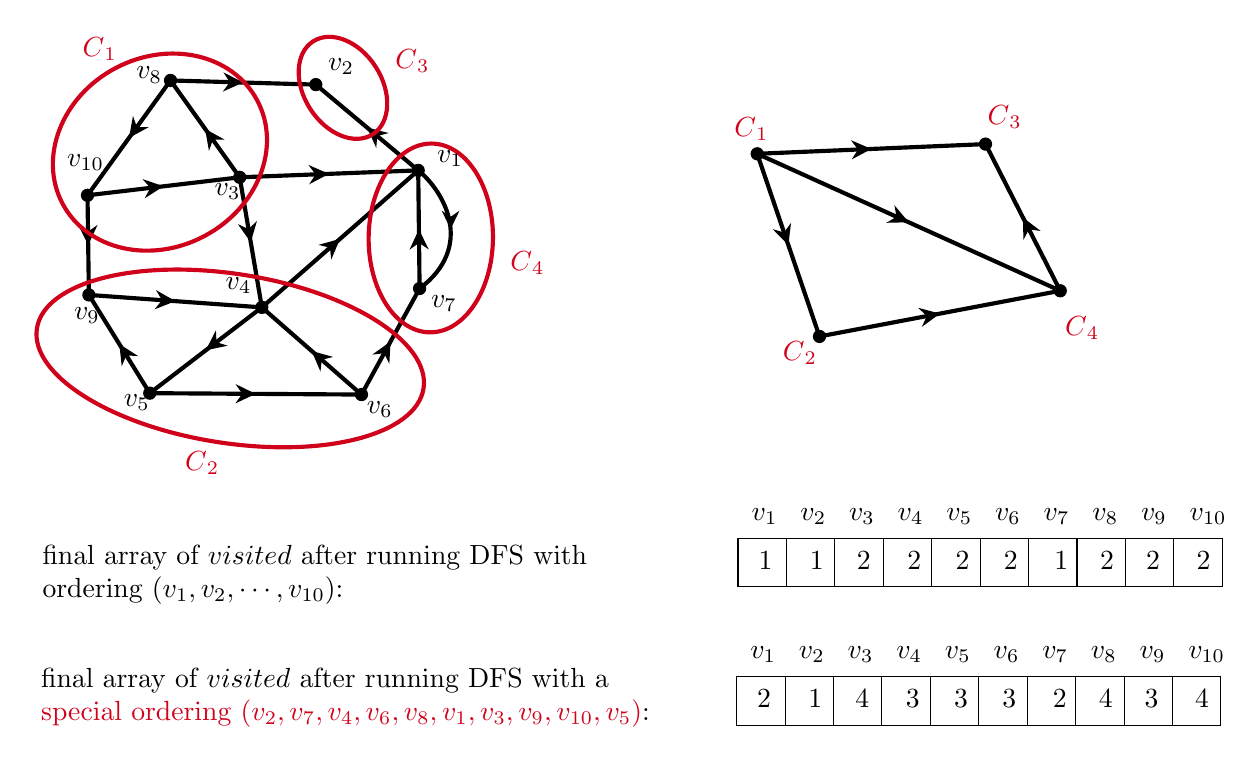
\begin{tikzpicture}[x=0.5pt,y=0.5pt,yscale=-1,xscale=1]
%uncomment if require: \path (0,553); %set diagram left start at 0, and has height of 553

%Flowchart: Connector [id:dp33314190657915177] 
\draw  [fill={rgb, 255:red, 0; green, 0; blue, 0 }  ,fill opacity=1 ] (137,52) .. controls (137,49.58) and (138.96,47.62) .. (141.38,47.62) .. controls (143.79,47.62) and (145.75,49.58) .. (145.75,52) .. controls (145.75,54.42) and (143.79,56.38) .. (141.38,56.38) .. controls (138.96,56.38) and (137,54.42) .. (137,52) -- cycle ;
%Flowchart: Connector [id:dp9493779383807376] 
\draw  [fill={rgb, 255:red, 0; green, 0; blue, 0 }  ,fill opacity=1 ] (242,55) .. controls (242,52.58) and (243.96,50.62) .. (246.38,50.62) .. controls (248.79,50.62) and (250.75,52.58) .. (250.75,55) .. controls (250.75,57.42) and (248.79,59.38) .. (246.38,59.38) .. controls (243.96,59.38) and (242,57.42) .. (242,55) -- cycle ;
%Flowchart: Connector [id:dp6669453073289408] 
\draw  [fill={rgb, 255:red, 0; green, 0; blue, 0 }  ,fill opacity=1 ] (122,278) .. controls (122,275.58) and (123.96,273.62) .. (126.38,273.62) .. controls (128.79,273.62) and (130.75,275.58) .. (130.75,278) .. controls (130.75,280.42) and (128.79,282.38) .. (126.38,282.38) .. controls (123.96,282.38) and (122,280.42) .. (122,278) -- cycle ;
%Flowchart: Connector [id:dp333713085025936] 
\draw  [fill={rgb, 255:red, 0; green, 0; blue, 0 }  ,fill opacity=1 ] (77,135) .. controls (77,132.58) and (78.96,130.62) .. (81.38,130.62) .. controls (83.79,130.62) and (85.75,132.58) .. (85.75,135) .. controls (85.75,137.42) and (83.79,139.38) .. (81.38,139.38) .. controls (78.96,139.38) and (77,137.42) .. (77,135) -- cycle ;
%Flowchart: Connector [id:dp9629725454572109] 
\draw  [fill={rgb, 255:red, 0; green, 0; blue, 0 }  ,fill opacity=1 ] (187,122) .. controls (187,119.58) and (188.96,117.62) .. (191.38,117.62) .. controls (193.79,117.62) and (195.75,119.58) .. (195.75,122) .. controls (195.75,124.42) and (193.79,126.38) .. (191.38,126.38) .. controls (188.96,126.38) and (187,124.42) .. (187,122) -- cycle ;
%Straight Lines [id:da6590518201146447] 
\draw [color={rgb, 255:red, 0; green, 0; blue, 0 }  ,draw opacity=1 ][line width=1.5]    (81.38,135) -- (141.38,52) ;
\draw [shift={(111.38,93.5)}, rotate = 305.86] [fill={rgb, 255:red, 0; green, 0; blue, 0 }  ,fill opacity=1 ][line width=0.08]  [draw opacity=0] (14.56,-6.99) -- (0,0) -- (14.56,6.99) -- (9.67,0) -- cycle    ;
%Straight Lines [id:da1177530387710749] 
\draw [color={rgb, 255:red, 0; green, 0; blue, 0 }  ,draw opacity=1 ][line width=1.5]    (126.38,278) -- (207.38,216) ;
\draw [shift={(166.88,247)}, rotate = 322.57] [fill={rgb, 255:red, 0; green, 0; blue, 0 }  ,fill opacity=1 ][line width=0.08]  [draw opacity=0] (14.56,-6.99) -- (0,0) -- (14.56,6.99) -- (9.67,0) -- cycle    ;
%Straight Lines [id:da8328235451162237] 
\draw [color={rgb, 255:red, 0; green, 0; blue, 0 }  ,draw opacity=1 ][line width=1.5]    (191.38,122) -- (81.38,135) ;
\draw [shift={(136.38,128.5)}, rotate = 173.26] [fill={rgb, 255:red, 0; green, 0; blue, 0 }  ,fill opacity=1 ][line width=0.08]  [draw opacity=0] (14.56,-6.99) -- (0,0) -- (14.56,6.99) -- (9.67,0) -- cycle    ;
%Straight Lines [id:da13491976799128524] 
\draw [color={rgb, 255:red, 0; green, 0; blue, 0 }  ,draw opacity=1 ][line width=1.5]    (126.38,278) -- (82.38,207) ;
\draw [shift={(104.38,242.5)}, rotate = 58.21] [fill={rgb, 255:red, 0; green, 0; blue, 0 }  ,fill opacity=1 ][line width=0.08]  [draw opacity=0] (14.56,-6.99) -- (0,0) -- (14.56,6.99) -- (9.67,0) -- cycle    ;
%Flowchart: Connector [id:dp015404259848177726] 
\draw  [fill={rgb, 255:red, 0; green, 0; blue, 0 }  ,fill opacity=1 ] (275,279) .. controls (275,276.58) and (276.96,274.62) .. (279.38,274.62) .. controls (281.79,274.62) and (283.75,276.58) .. (283.75,279) .. controls (283.75,281.42) and (281.79,283.38) .. (279.38,283.38) .. controls (276.96,283.38) and (275,281.42) .. (275,279) -- cycle ;
%Straight Lines [id:da9050593875476026] 
\draw [color={rgb, 255:red, 0; green, 0; blue, 0 }  ,draw opacity=1 ][line width=1.5]    (279.38,279) -- (321.38,202.38) ;
\draw [shift={(300.38,240.69)}, rotate = 118.73] [fill={rgb, 255:red, 0; green, 0; blue, 0 }  ,fill opacity=1 ][line width=0.08]  [draw opacity=0] (14.56,-6.99) -- (0,0) -- (14.56,6.99) -- (9.67,0) -- cycle    ;
%Straight Lines [id:da6930328339194429] 
\draw [color={rgb, 255:red, 0; green, 0; blue, 0 }  ,draw opacity=1 ][line width=1.5]    (126.38,278) -- (279.38,279) ;
\draw [shift={(202.88,278.5)}, rotate = 180.37] [fill={rgb, 255:red, 0; green, 0; blue, 0 }  ,fill opacity=1 ][line width=0.08]  [draw opacity=0] (14.56,-6.99) -- (0,0) -- (14.56,6.99) -- (9.67,0) -- cycle    ;
%Flowchart: Connector [id:dp8561555389036362] 
\draw  [fill={rgb, 255:red, 0; green, 0; blue, 0 }  ,fill opacity=1 ] (317,202.38) .. controls (317,199.96) and (318.96,198) .. (321.38,198) .. controls (323.79,198) and (325.75,199.96) .. (325.75,202.38) .. controls (325.75,204.79) and (323.79,206.75) .. (321.38,206.75) .. controls (318.96,206.75) and (317,204.79) .. (317,202.38) -- cycle ;
%Straight Lines [id:da4194772983165912] 
\draw [color={rgb, 255:red, 0; green, 0; blue, 0 }  ,draw opacity=1 ][line width=1.5]    (321.38,202.38) -- (320.38,117) ;
\draw [shift={(320.88,159.69)}, rotate = 89.33] [fill={rgb, 255:red, 0; green, 0; blue, 0 }  ,fill opacity=1 ][line width=0.08]  [draw opacity=0] (14.56,-6.99) -- (0,0) -- (14.56,6.99) -- (9.67,0) -- cycle    ;
%Straight Lines [id:da26627336015658065] 
\draw [color={rgb, 255:red, 0; green, 0; blue, 0 }  ,draw opacity=1 ][line width=1.5]    (320.38,117) -- (246.38,55) ;
\draw [shift={(283.38,86)}, rotate = 39.96] [fill={rgb, 255:red, 0; green, 0; blue, 0 }  ,fill opacity=1 ][line width=0.08]  [draw opacity=0] (14.56,-6.99) -- (0,0) -- (14.56,6.99) -- (9.67,0) -- cycle    ;
%Straight Lines [id:da6540321478063363] 
\draw [color={rgb, 255:red, 0; green, 0; blue, 0 }  ,draw opacity=1 ][line width=1.5]    (141.38,52) -- (191.38,122) ;
\draw [shift={(166.38,87)}, rotate = 54.46] [fill={rgb, 255:red, 0; green, 0; blue, 0 }  ,fill opacity=1 ][line width=0.08]  [draw opacity=0] (14.56,-6.99) -- (0,0) -- (14.56,6.99) -- (9.67,0) -- cycle    ;
%Straight Lines [id:da980763773394733] 
\draw [color={rgb, 255:red, 0; green, 0; blue, 0 }  ,draw opacity=1 ][line width=1.5]    (207.38,216) -- (279.38,279) ;
\draw [shift={(243.38,247.5)}, rotate = 41.19] [fill={rgb, 255:red, 0; green, 0; blue, 0 }  ,fill opacity=1 ][line width=0.08]  [draw opacity=0] (14.56,-6.99) -- (0,0) -- (14.56,6.99) -- (9.67,0) -- cycle    ;
%Flowchart: Connector [id:dp884579398191617] 
\draw  [fill={rgb, 255:red, 0; green, 0; blue, 0 }  ,fill opacity=1 ] (203,216) .. controls (203,213.58) and (204.96,211.62) .. (207.38,211.62) .. controls (209.79,211.62) and (211.75,213.58) .. (211.75,216) .. controls (211.75,218.42) and (209.79,220.38) .. (207.38,220.38) .. controls (204.96,220.38) and (203,218.42) .. (203,216) -- cycle ;
%Flowchart: Connector [id:dp3352413725395753] 
\draw  [fill={rgb, 255:red, 0; green, 0; blue, 0 }  ,fill opacity=1 ] (78,207) .. controls (78,204.58) and (79.96,202.62) .. (82.38,202.62) .. controls (84.79,202.62) and (86.75,204.58) .. (86.75,207) .. controls (86.75,209.42) and (84.79,211.38) .. (82.38,211.38) .. controls (79.96,211.38) and (78,209.42) .. (78,207) -- cycle ;
%Flowchart: Connector [id:dp01230167588576514] 
\draw  [fill={rgb, 255:red, 0; green, 0; blue, 0 }  ,fill opacity=1 ] (316,117) .. controls (316,114.58) and (317.96,112.62) .. (320.38,112.62) .. controls (322.79,112.62) and (324.75,114.58) .. (324.75,117) .. controls (324.75,119.42) and (322.79,121.38) .. (320.38,121.38) .. controls (317.96,121.38) and (316,119.42) .. (316,117) -- cycle ;
%Straight Lines [id:da2185567480823013] 
\draw [color={rgb, 255:red, 0; green, 0; blue, 0 }  ,draw opacity=1 ][line width=1.5]    (207.38,216) -- (82.38,207) ;
\draw [shift={(144.88,211.5)}, rotate = 184.12] [fill={rgb, 255:red, 0; green, 0; blue, 0 }  ,fill opacity=1 ][line width=0.08]  [draw opacity=0] (14.56,-6.99) -- (0,0) -- (14.56,6.99) -- (9.67,0) -- cycle    ;
%Curve Lines [id:da3916533808212287] 
\draw [line width=1.5]    (321.38,202.38) .. controls (361.38,172.38) and (339.68,132.52) .. (320.38,117) ;
\draw [shift={(343.77,159.48)}, rotate = 270.05] [fill={rgb, 255:red, 0; green, 0; blue, 0 }  ][line width=0.08]  [draw opacity=0] (13.4,-6.43) -- (0,0) -- (13.4,6.44) -- (8.9,0) -- cycle    ;
%Straight Lines [id:da9071388879776039] 
\draw [color={rgb, 255:red, 0; green, 0; blue, 0 }  ,draw opacity=1 ][line width=1.5]    (207.38,216) -- (320.38,117) ;
\draw [shift={(263.88,166.5)}, rotate = 138.78] [fill={rgb, 255:red, 0; green, 0; blue, 0 }  ,fill opacity=1 ][line width=0.08]  [draw opacity=0] (14.56,-6.99) -- (0,0) -- (14.56,6.99) -- (9.67,0) -- cycle    ;
%Straight Lines [id:da17399207464778044] 
\draw [color={rgb, 255:red, 0; green, 0; blue, 0 }  ,draw opacity=1 ][line width=1.5]    (191.38,122) -- (207.38,216) ;
\draw [shift={(199.38,169)}, rotate = 260.34] [fill={rgb, 255:red, 0; green, 0; blue, 0 }  ,fill opacity=1 ][line width=0.08]  [draw opacity=0] (14.56,-6.99) -- (0,0) -- (14.56,6.99) -- (9.67,0) -- cycle    ;
%Straight Lines [id:da8016859457087312] 
\draw [color={rgb, 255:red, 0; green, 0; blue, 0 }  ,draw opacity=1 ][line width=1.5]    (81.38,135) -- (82.38,207) ;
\draw [shift={(81.88,171)}, rotate = 269.2] [fill={rgb, 255:red, 0; green, 0; blue, 0 }  ,fill opacity=1 ][line width=0.08]  [draw opacity=0] (14.56,-6.99) -- (0,0) -- (14.56,6.99) -- (9.67,0) -- cycle    ;
%Straight Lines [id:da8138783684306082] 
\draw [color={rgb, 255:red, 0; green, 0; blue, 0 }  ,draw opacity=1 ][line width=1.5]    (191.38,122) -- (320.38,117) ;
\draw [shift={(255.88,119.5)}, rotate = 177.78] [fill={rgb, 255:red, 0; green, 0; blue, 0 }  ,fill opacity=1 ][line width=0.08]  [draw opacity=0] (14.56,-6.99) -- (0,0) -- (14.56,6.99) -- (9.67,0) -- cycle    ;
%Straight Lines [id:da24392431611835252] 
\draw [color={rgb, 255:red, 0; green, 0; blue, 0 }  ,draw opacity=1 ][line width=1.5]    (141.38,52) -- (246.38,55) ;
\draw [shift={(193.88,53.5)}, rotate = 181.64] [fill={rgb, 255:red, 0; green, 0; blue, 0 }  ,fill opacity=1 ][line width=0.08]  [draw opacity=0] (14.56,-6.99) -- (0,0) -- (14.56,6.99) -- (9.67,0) -- cycle    ;
%Shape: Ellipse [id:dp837267975011143] 
\draw  [color={rgb, 255:red, 208; green, 2; blue, 27 }  ,draw opacity=1 ][line width=1.5]  (63.39,141.12) .. controls (45.61,107.62) and (62.68,63.75) .. (101.52,43.13) .. controls (140.37,22.52) and (186.27,32.96) .. (204.05,66.45) .. controls (221.83,99.95) and (204.76,143.82) .. (165.91,164.44) .. controls (127.07,185.06) and (81.17,174.61) .. (63.39,141.12) -- cycle ;
%Shape: Ellipse [id:dp6301102730017264] 
\draw  [color={rgb, 255:red, 208; green, 2; blue, 27 }  ,draw opacity=1 ][line width=1.5]  (44.82,231.18) .. controls (50.01,197.81) and (116.75,180.47) .. (193.91,192.46) .. controls (271.06,204.44) and (329.4,241.21) .. (324.22,274.58) .. controls (319.04,307.95) and (252.29,325.29) .. (175.14,313.3) .. controls (97.98,301.32) and (39.64,264.55) .. (44.82,231.18) -- cycle ;
%Shape: Ellipse [id:dp9534249176688527] 
\draw  [color={rgb, 255:red, 208; green, 2; blue, 27 }  ,draw opacity=1 ][line width=1.5]  (330.2,97.61) .. controls (355.02,97.88) and (374.8,128.63) .. (374.4,166.31) .. controls (374,203.98) and (353.56,234.31) .. (328.75,234.04) .. controls (303.94,233.78) and (284.15,203.02) .. (284.55,165.35) .. controls (284.96,127.68) and (305.39,97.35) .. (330.2,97.61) -- cycle ;
%Shape: Ellipse [id:dp8449632734349601] 
\draw  [color={rgb, 255:red, 208; green, 2; blue, 27 }  ,draw opacity=1 ][line width=1.5]  (244.45,23.74) .. controls (257.53,15.36) and (277.77,23.6) .. (289.66,42.15) .. controls (301.55,60.71) and (300.58,82.54) .. (287.5,90.92) .. controls (274.42,99.3) and (254.19,91.05) .. (242.3,72.5) .. controls (230.41,53.95) and (231.38,32.12) .. (244.45,23.74) -- cycle ;
%Flowchart: Connector [id:dp603695290762529] 
\draw  [fill={rgb, 255:red, 0; green, 0; blue, 0 }  ,fill opacity=1 ] (606,237) .. controls (606,234.58) and (607.96,232.62) .. (610.38,232.62) .. controls (612.79,232.62) and (614.75,234.58) .. (614.75,237) .. controls (614.75,239.42) and (612.79,241.38) .. (610.38,241.38) .. controls (607.96,241.38) and (606,239.42) .. (606,237) -- cycle ;
%Straight Lines [id:da27444933364712354] 
\draw [color={rgb, 255:red, 0; green, 0; blue, 0 }  ,draw opacity=1 ][line width=1.5]    (784.38,204) -- (565.38,105) ;
\draw [shift={(674.88,154.5)}, rotate = 204.33] [fill={rgb, 255:red, 0; green, 0; blue, 0 }  ,fill opacity=1 ][line width=0.08]  [draw opacity=0] (14.56,-6.99) -- (0,0) -- (14.56,6.99) -- (9.67,0) -- cycle    ;
%Straight Lines [id:da6238918789957093] 
\draw [color={rgb, 255:red, 0; green, 0; blue, 0 }  ,draw opacity=1 ][line width=1.5]    (784.38,204) -- (730.38,98) ;
\draw [shift={(757.38,151)}, rotate = 63] [fill={rgb, 255:red, 0; green, 0; blue, 0 }  ,fill opacity=1 ][line width=0.08]  [draw opacity=0] (14.56,-6.99) -- (0,0) -- (14.56,6.99) -- (9.67,0) -- cycle    ;
%Flowchart: Connector [id:dp07658274147850641] 
\draw  [fill={rgb, 255:red, 0; green, 0; blue, 0 }  ,fill opacity=1 ] (726,98) .. controls (726,95.58) and (727.96,93.62) .. (730.38,93.62) .. controls (732.79,93.62) and (734.75,95.58) .. (734.75,98) .. controls (734.75,100.42) and (732.79,102.38) .. (730.38,102.38) .. controls (727.96,102.38) and (726,100.42) .. (726,98) -- cycle ;
%Flowchart: Connector [id:dp6792415791877835] 
\draw  [fill={rgb, 255:red, 0; green, 0; blue, 0 }  ,fill opacity=1 ] (561,105) .. controls (561,102.58) and (562.96,100.62) .. (565.38,100.62) .. controls (567.79,100.62) and (569.75,102.58) .. (569.75,105) .. controls (569.75,107.42) and (567.79,109.38) .. (565.38,109.38) .. controls (562.96,109.38) and (561,107.42) .. (561,105) -- cycle ;
%Straight Lines [id:da6954252151831065] 
\draw [color={rgb, 255:red, 0; green, 0; blue, 0 }  ,draw opacity=1 ][line width=1.5]    (610.38,237) -- (565.38,105) ;
\draw [shift={(587.88,171)}, rotate = 251.18] [fill={rgb, 255:red, 0; green, 0; blue, 0 }  ,fill opacity=1 ][line width=0.08]  [draw opacity=0] (14.56,-6.99) -- (0,0) -- (14.56,6.99) -- (9.67,0) -- cycle    ;
%Straight Lines [id:da21094314981608042] 
\draw [color={rgb, 255:red, 0; green, 0; blue, 0 }  ,draw opacity=1 ][line width=1.5]    (565.38,105) -- (730.38,98) ;
\draw [shift={(647.88,101.5)}, rotate = 177.57] [fill={rgb, 255:red, 0; green, 0; blue, 0 }  ,fill opacity=1 ][line width=0.08]  [draw opacity=0] (14.56,-6.99) -- (0,0) -- (14.56,6.99) -- (9.67,0) -- cycle    ;
%Flowchart: Connector [id:dp8786817451944372] 
\draw  [fill={rgb, 255:red, 0; green, 0; blue, 0 }  ,fill opacity=1 ] (780,204) .. controls (780,201.58) and (781.96,199.62) .. (784.38,199.62) .. controls (786.79,199.62) and (788.75,201.58) .. (788.75,204) .. controls (788.75,206.42) and (786.79,208.38) .. (784.38,208.38) .. controls (781.96,208.38) and (780,206.42) .. (780,204) -- cycle ;
%Straight Lines [id:da6613494332963039] 
\draw [color={rgb, 255:red, 0; green, 0; blue, 0 }  ,draw opacity=1 ][line width=1.5]    (784.38,204) -- (610.38,237) ;
\draw [shift={(697.38,220.5)}, rotate = 169.26] [fill={rgb, 255:red, 0; green, 0; blue, 0 }  ,fill opacity=1 ][line width=0.08]  [draw opacity=0] (14.56,-6.99) -- (0,0) -- (14.56,6.99) -- (9.67,0) -- cycle    ;
%Shape: Grid [id:dp7216183755073775] 
\draw  [draw opacity=0] (551.5,382.87) -- (901.5,382.87) -- (901.5,417.87) -- (551.5,417.87) -- cycle ; \draw   (586.5,382.87) -- (586.5,417.87)(621.5,382.87) -- (621.5,417.87)(656.5,382.87) -- (656.5,417.87)(691.5,382.87) -- (691.5,417.87)(726.5,382.87) -- (726.5,417.87)(761.5,382.87) -- (761.5,417.87)(796.5,382.87) -- (796.5,417.87)(831.5,382.87) -- (831.5,417.87)(866.5,382.87) -- (866.5,417.87) ; \draw    ; \draw   (551.5,382.87) -- (901.5,382.87) -- (901.5,417.87) -- (551.5,417.87) -- cycle ;
%Shape: Grid [id:dp08811438988655107] 
\draw  [draw opacity=0] (550.5,482.87) -- (900.5,482.87) -- (900.5,517.87) -- (550.5,517.87) -- cycle ; \draw   (585.5,482.87) -- (585.5,517.87)(620.5,482.87) -- (620.5,517.87)(655.5,482.87) -- (655.5,517.87)(690.5,482.87) -- (690.5,517.87)(725.5,482.87) -- (725.5,517.87)(760.5,482.87) -- (760.5,517.87)(795.5,482.87) -- (795.5,517.87)(830.5,482.87) -- (830.5,517.87)(865.5,482.87) -- (865.5,517.87) ; \draw    ; \draw   (550.5,482.87) -- (900.5,482.87) -- (900.5,517.87) -- (550.5,517.87) -- cycle ;

% Text Node
\draw (332.2,100.61) node [anchor=north west][inner sep=0.75pt]   [align=left] {$\displaystyle v_{1}$};
% Text Node
\draw (171.38,124.38) node [anchor=north west][inner sep=0.75pt]   [align=left] {$\displaystyle v_{3}$};
% Text Node
\draw (105.75,277) node [anchor=north west][inner sep=0.75pt]   [align=left] {$\displaystyle v_{5}$};
% Text Node
\draw (179.38,192.38) node [anchor=north west][inner sep=0.75pt]   [align=left] {$\displaystyle v_{4}$};
% Text Node
\draw (253.38,34.38) node [anchor=north west][inner sep=0.75pt]   [align=left] {$\displaystyle v_{2}$};
% Text Node
\draw (69.75,214.35) node [anchor=north west][inner sep=0.75pt]   [align=left] {$\displaystyle v_{9}$};
% Text Node
\draw (327.75,205.38) node [anchor=north west][inner sep=0.75pt]   [align=left] {$\displaystyle v_{7}$};
% Text Node
\draw (281.38,282) node [anchor=north west][inner sep=0.75pt]   [align=left] {$\displaystyle v_{6}$};
% Text Node
\draw (114.75,40.35) node [anchor=north west][inner sep=0.75pt]   [align=left] {$\displaystyle v_{8}$};
% Text Node
\draw (64.75,103.35) node [anchor=north west][inner sep=0.75pt]   [align=left] {$\displaystyle v_{10}$};
% Text Node
\draw (76,19) node [anchor=north west][inner sep=0.75pt]   [align=left] {$\displaystyle \textcolor[rgb]{0.82,0.01,0.11}{C}\textcolor[rgb]{0.82,0.01,0.11}{_{1}}$};
% Text Node
\draw (150,318) node [anchor=north west][inner sep=0.75pt]   [align=left] {$\displaystyle \textcolor[rgb]{0.82,0.01,0.11}{C}\textcolor[rgb]{0.82,0.01,0.11}{_{2}}$};
% Text Node
\draw (385,174) node [anchor=north west][inner sep=0.75pt]   [align=left] {$\displaystyle \textcolor[rgb]{0.82,0.01,0.11}{C}\textcolor[rgb]{0.82,0.01,0.11}{_{4}}$};
% Text Node
\draw (302,28) node [anchor=north west][inner sep=0.75pt]   [align=left] {$\displaystyle \textcolor[rgb]{0.82,0.01,0.11}{C}\textcolor[rgb]{0.82,0.01,0.11}{_{3}}$};
% Text Node
\draw (582,239) node [anchor=north west][inner sep=0.75pt]   [align=left] {$\displaystyle \textcolor[rgb]{0.82,0.01,0.11}{C}\textcolor[rgb]{0.82,0.01,0.11}{_{2}}$};
% Text Node
\draw (786,221) node [anchor=north west][inner sep=0.75pt]   [align=left] {$\displaystyle \textcolor[rgb]{0.82,0.01,0.11}{C}\textcolor[rgb]{0.82,0.01,0.11}{_{4}}$};
% Text Node
\draw (547,77) node [anchor=north west][inner sep=0.75pt]   [align=left] {$\displaystyle \textcolor[rgb]{0.82,0.01,0.11}{C}\textcolor[rgb]{0.82,0.01,0.11}{_{1}}$};
% Text Node
\draw (730,68) node [anchor=north west][inner sep=0.75pt]   [align=left] {$\displaystyle \textcolor[rgb]{0.82,0.01,0.11}{C}\textcolor[rgb]{0.82,0.01,0.11}{_{3}}$};
% Text Node
\draw (47,385.93) node [anchor=north west][inner sep=0.75pt]   [align=left] {final array of $\displaystyle visited$ after running DFS with\\ordering $\displaystyle ( v_{1} ,v_{2} ,\cdots ,v_{10})$:};
% Text Node
\draw (672,390.37) node [anchor=north west][inner sep=0.75pt]   [align=left] {$\displaystyle 2$};
% Text Node
\draw (706.83,390.37) node [anchor=north west][inner sep=0.75pt]   [align=left] {$\displaystyle 2$};
% Text Node
\draw (741.66,390.37) node [anchor=north west][inner sep=0.75pt]   [align=left] {$\displaystyle 2$};
% Text Node
\draw (844.49,390.37) node [anchor=north west][inner sep=0.75pt]   [align=left] {$\displaystyle 2$};
% Text Node
\draw (811.32,390.37) node [anchor=north west][inner sep=0.75pt]   [align=left] {$\displaystyle 2$};
% Text Node
\draw (778.15,390.37) node [anchor=north west][inner sep=0.75pt]   [align=left] {$\displaystyle 1$};
% Text Node
\draw (881,390.37) node [anchor=north west][inner sep=0.75pt]   [align=left] {$\displaystyle 2$};
% Text Node
\draw (564.49,390.37) node [anchor=north west][inner sep=0.75pt]   [align=left] {$\displaystyle 1$};
% Text Node
\draw (601.49,390.37) node [anchor=north west][inner sep=0.75pt]   [align=left] {$\displaystyle 1$};
% Text Node
\draw (635.49,390.37) node [anchor=north west][inner sep=0.75pt]   [align=left] {$\displaystyle 2$};
% Text Node
\draw (665,359.37) node [anchor=north west][inner sep=0.75pt]   [align=left] {$\displaystyle v_{4}$};
% Text Node
\draw (700.17,359.37) node [anchor=north west][inner sep=0.75pt]   [align=left] {$\displaystyle v_{5}$};
% Text Node
\draw (735.34,359.37) node [anchor=north west][inner sep=0.75pt]   [align=left] {$\displaystyle v_{6}$};
% Text Node
\draw (840.85,359.37) node [anchor=north west][inner sep=0.75pt]   [align=left] {$\displaystyle v_{9}$};
% Text Node
\draw (805.68,359.37) node [anchor=north west][inner sep=0.75pt]   [align=left] {$\displaystyle v_{8}$};
% Text Node
\draw (770.51,359.37) node [anchor=north west][inner sep=0.75pt]   [align=left] {$\displaystyle v_{7}$};
% Text Node
\draw (876,359.37) node [anchor=north west][inner sep=0.75pt]   [align=left] {$\displaystyle v_{10}$};
% Text Node
\draw (559.49,359.37) node [anchor=north west][inner sep=0.75pt]   [align=left] {$\displaystyle v_{1}$};
% Text Node
\draw (594.66,359.37) node [anchor=north west][inner sep=0.75pt]   [align=left] {$\displaystyle v_{2}$};
% Text Node
\draw (629.83,359.37) node [anchor=north west][inner sep=0.75pt]   [align=left] {$\displaystyle v_{3}$};
% Text Node
\draw (46,474.93) node [anchor=north west][inner sep=0.75pt]   [align=left] {final array of $\displaystyle visited$ after running DFS with a \\\textcolor[rgb]{0.82,0.01,0.11}{special ordering }$\displaystyle \textcolor[rgb]{0.82,0.01,0.11}{( v_{2} ,v_{7} ,v_{4} ,v_{6} ,v_{8} ,v_{1} ,v_{3} ,v_{9} ,v_{10} ,v_{5})}$:};
% Text Node
\draw (671,490.37) node [anchor=north west][inner sep=0.75pt]   [align=left] {$\displaystyle 3$};
% Text Node
\draw (705.83,490.37) node [anchor=north west][inner sep=0.75pt]   [align=left] {$\displaystyle 3$};
% Text Node
\draw (740.66,490.37) node [anchor=north west][inner sep=0.75pt]   [align=left] {$\displaystyle 3$};
% Text Node
\draw (843.49,490.37) node [anchor=north west][inner sep=0.75pt]   [align=left] {$\displaystyle 3$};
% Text Node
\draw (810.32,490.37) node [anchor=north west][inner sep=0.75pt]   [align=left] {$\displaystyle 4$};
% Text Node
\draw (777.15,490.37) node [anchor=north west][inner sep=0.75pt]   [align=left] {$\displaystyle 2$};
% Text Node
\draw (880,490.37) node [anchor=north west][inner sep=0.75pt]   [align=left] {$\displaystyle 4$};
% Text Node
\draw (563.49,490.37) node [anchor=north west][inner sep=0.75pt]   [align=left] {$\displaystyle 2$};
% Text Node
\draw (600.49,490.37) node [anchor=north west][inner sep=0.75pt]   [align=left] {$\displaystyle 1$};
% Text Node
\draw (634.49,490.37) node [anchor=north west][inner sep=0.75pt]   [align=left] {$\displaystyle 4$};
% Text Node
\draw (664,459.37) node [anchor=north west][inner sep=0.75pt]   [align=left] {$\displaystyle v_{4}$};
% Text Node
\draw (699.17,459.37) node [anchor=north west][inner sep=0.75pt]   [align=left] {$\displaystyle v_{5}$};
% Text Node
\draw (734.34,459.37) node [anchor=north west][inner sep=0.75pt]   [align=left] {$\displaystyle v_{6}$};
% Text Node
\draw (839.85,459.37) node [anchor=north west][inner sep=0.75pt]   [align=left] {$\displaystyle v_{9}$};
% Text Node
\draw (804.68,459.37) node [anchor=north west][inner sep=0.75pt]   [align=left] {$\displaystyle v_{8}$};
% Text Node
\draw (769.51,459.37) node [anchor=north west][inner sep=0.75pt]   [align=left] {$\displaystyle v_{7}$};
% Text Node
\draw (875,459.37) node [anchor=north west][inner sep=0.75pt]   [align=left] {$\displaystyle v_{10}$};
% Text Node
\draw (558.49,459.37) node [anchor=north west][inner sep=0.75pt]   [align=left] {$\displaystyle v_{1}$};
% Text Node
\draw (593.66,459.37) node [anchor=north west][inner sep=0.75pt]   [align=left] {$\displaystyle v_{2}$};
% Text Node
\draw (628.83,459.37) node [anchor=north west][inner sep=0.75pt]   [align=left] {$\displaystyle v_{3}$};


\end{tikzpicture}

}
\caption{Run the DFS algorithm with an arbitrary ordering (introduced in Lecture A9) and a special ordering~(pseudo-code given below) on above example.}
\label{fig:dfs-meta}
\end{figure}

How to fix this issue? The idea is to use a \emph{special ordering} of vertices, instead of an arbitrary ordering, in above DFS.
This special ordering should allow us to determine connected component one by one. Hence, the first vertex we explore in DFS,
should be one vertex in a \emph{sink} component of the meta-graph. In Figure~\ref{fig:dfs-meta}, the only sink component is $C_3$,
and since there is only one vertex in $C_3$, we should start with exploring $v_2$.
Clearly, exploring $v_2$ will exactly determine the single connected component $C_2$.
Next, after $C_3$ is determined, the next component we can determine is again a sink component after removing $C_3$ from the meta-graph.
It is $C_4$. So, the next vertex the DFS should explore must be $v_1$ or $v_7$. It does matter which one we pick; let's assume we pick $v_7$~(and it
does not matter where $v_1$ is in the ordering as long as it is after $v_2$ and $v_7$).
Clearly, exploring $v_2$ will exactly determine the single connected component $C_4$---see the visited array.
The next component we can determine is again a sink component after removing $C_3$ and $C_4$ from the meta-graph.
It is $C_2$. So, the next vertex the DFS should explore must be in $\{v_4, v_5,v_6,v_9\}$. 
And it does matter which one we pick neither the ordering of remaining ones as long as they are behind the one we pick.
Let's say we pick $v_4$. Clearly, exploring $v_4$ will exactly determine the single connected component $C_2$.
Now the only component remaining is $C_1$ after removing $C_2$, $C_3$ and $C_4$ from the meta-graph.
So, the next vertex the DFS should explore must be in $\{v_3, v_8, v_{10}\}$. 
Let's say we pick $v_8$. Clearly, exploring $v_8$ will exactly determine the last connected component $C_1$.


To abtract above observation, the determined connected components with above DFS
forms a reverse-linearization of the meta-graph.
Therefore, the special ordering of vertices should satisfy this condition:
\emph{the ordering of connected components sorted by their first appearance in the special ordering of vertices
should form a reverse-linearization of the meta-graph}.
And if the special ordering of vertices satisfies this condition, the DFS algorithm will work---it will identify
all connected components.

Again see Figure~\ref{fig:dfs-meta}, the ordering 
$( v_{2} ,v_{7} ,v_{4} ,v_{6} ,v_{8} ,v_{1} ,v_{3} ,v_{9} ,v_{10} ,v_{5})$ satisfies above condition.
To see that, the corresponding list of connected components is 
$(C_3, C_4, C_2, C_2, C_1, C_4, C_1, C_2, C_1, C_2)$,
and hence the ordering of their first appearance is $(C_3, C_4, C_2, C_1)$ which is indeed a reviers-linearization of the meta-graph.

\begin{minipage}{0.8\textwidth}
	\aaA {8}{function DFS ($G = (V, E)$)}\xxx
	\aab {num-cc = 0;}\xxx
	\aaB {5}{for \textcolor{blue}{$v_i$ in a specific order}}\xxx
	\aaC {3}{if ($visited[i] = 0$)}\xxx
	\aad {num-cc = num-cc + 1;}\xxx
	\aad {explore ($G, v_j$);}\xxx
	\aac {end if;}\xxx
	\aab {end for;}\xxx
	\aaa {end algorithm;}\xxx
\end{minipage}

\begin{minipage}{0.8\textwidth}
	\aaA {5}{function explore ($G = (V, E), v_i \in V$)}\xxx
	\aab {$visited[i] = $ num-cc;}\xxx
	\aaB {2}{for any edge $(v_i, v_j) \in E$}\xxx
	\aac {if ($visited[j] = 0$): explore ($G, v_j$);}\xxx
	\aab {end for;}\xxx
	\aaa {end algorithm;}\xxx
\end{minipage}

To summarize, the algorithm to identify connected components of directed graphs
is essentially the same with that for undirected graphs~(introduced in Lecture~A9, copied above), 
except a single line of difference~(marked blue): for directed graphs,
we need to explore vertices in a specific order that satisfy above condition,
while for undirected graphs, we can explore all vertices in any arbitrary order.

How to find an ordering of vertices that satisfy above condition?
We need a combination of two techniques: DFS-with-timing and reverse-graph.



\subsection*{DFS with Timing}

%We now design another variant of DFS algorithm, which will be used to construct the linerization of DAGs, while also
%can construct meta-graphs for (general) directed graphs. This variant of DFS, called 
The DFS-with-timing is a variant of DFS, which uses the following
data structures~(we assume $n = |V|$):

\vspace*{-\topsep}
\begin{enumerate}
\item variable clock servers as a timer that stores the current time;
\item binary array $visited[1..n]$, where $visited[i]$ indicates if $v[i]$ has been explored, $1 \le i \le n$;
\item array $pre[1..n]$, where $pre[i]$ records the time of starting exploring $v_i$, $1 \le i \le n$;
\item array $post[1..n]$, where $post[i]$ records the time of finishing exploring $v_i$, $1 \le i \le n$;
\item array $postlist$, stores the vertices in \textcolor{blue}{decreasing} order of $post[\cdot]$.
\end{enumerate}

The pseudo-code of DFS with timing is given below.

\begin{minipage}{0.8\textwidth}
	\aaA {5}{function DFS-with-timing ($G = (V, E)$)}\xxx
	\aab {$clock = 1$;}\xxx
	\aaB {2}{for $i = 1 \to |V|$}\xxx
	\aac {if ($visited[i] = 0$): explore ($G, v_i$);}\xxx
	\aab {end for;}\xxx
	\aaa {end algorithm;}\xxx
\end{minipage}

\begin{minipage}{0.8\textwidth}
	\aaA {10}{function explore ($G = (V, E), v_i \in V$)}\xxx
	\aab {$visited[i] = 1$;}\xxx
	\aab {$pre[i] = clock$;}\xxx
	\aab {$clock++$;}\xxx
	\aaB {2}{for any edge $(v_i, v_j) \in E$}\xxx
	\aac {if ($visited[j] = 0$): explore ($G, v_j$);}\xxx
	\aab {end for;}\xxx
	\aab {$post[i] = clock$;}\xxx
	\aab {$clock++$;}\xxx
	\aab {add $v_i$ to the \textcolor{blue}{front} of $postlist$;}\xxx
	\aaa {end algorithm;}\xxx
\end{minipage}

An example of running DFS with timing is given below.
Notice that the DFS searching partitions all edges into two categories:
solid edges $(u,v)$ implies that $v$ is visited for the first time~(and therefore explore $v$ will start right now),
while dashed edges $(u,v)$ implies that at that time $v$ has been visited already~(and therefore $v$ will be skipped and the next adjacent
vertex of $u$ will be examined in the for-loop). 

\begin{figure}[h!]
\centering{

\tikzset{every picture/.style={line width=0.75pt}} %set default line width to 0.75pt        

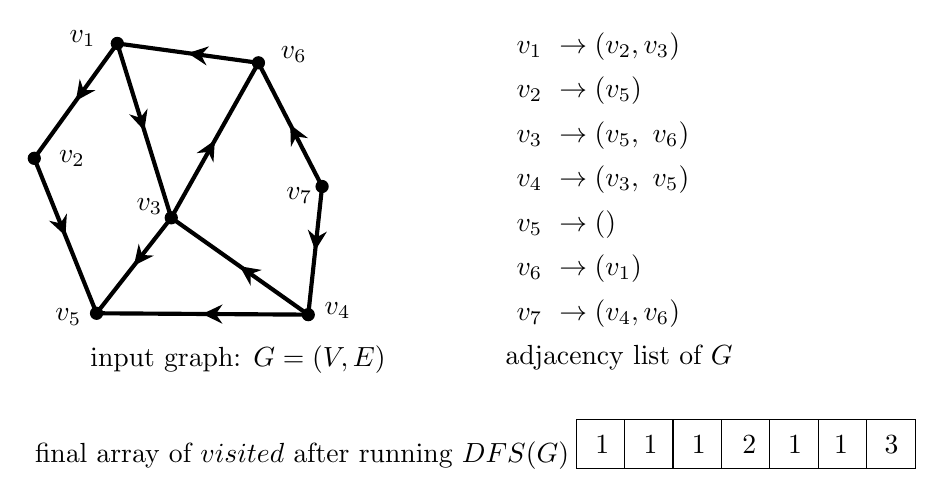
\begin{tikzpicture}[x=0.5pt,y=0.5pt,yscale=-1,xscale=1]
%uncomment if require: \path (0,342); %set diagram left start at 0, and has height of 342

%Flowchart: Connector [id:dp9968125919431555] 
\draw  [fill={rgb, 255:red, 0; green, 0; blue, 0 }  ,fill opacity=1 ] (78,14) .. controls (78,11.58) and (79.96,9.62) .. (82.38,9.62) .. controls (84.79,9.62) and (86.75,11.58) .. (86.75,14) .. controls (86.75,16.42) and (84.79,18.38) .. (82.38,18.38) .. controls (79.96,18.38) and (78,16.42) .. (78,14) -- cycle ;
%Flowchart: Connector [id:dp31888007270335605] 
\draw  [fill={rgb, 255:red, 0; green, 0; blue, 0 }  ,fill opacity=1 ] (180,28) .. controls (180,25.58) and (181.96,23.62) .. (184.38,23.62) .. controls (186.79,23.62) and (188.75,25.58) .. (188.75,28) .. controls (188.75,30.42) and (186.79,32.38) .. (184.38,32.38) .. controls (181.96,32.38) and (180,30.42) .. (180,28) -- cycle ;
%Flowchart: Connector [id:dp7333018163719219] 
\draw  [fill={rgb, 255:red, 0; green, 0; blue, 0 }  ,fill opacity=1 ] (63,209) .. controls (63,206.58) and (64.96,204.62) .. (67.38,204.62) .. controls (69.79,204.62) and (71.75,206.58) .. (71.75,209) .. controls (71.75,211.42) and (69.79,213.38) .. (67.38,213.38) .. controls (64.96,213.38) and (63,211.42) .. (63,209) -- cycle ;
%Flowchart: Connector [id:dp3353783499113435] 
\draw  [fill={rgb, 255:red, 0; green, 0; blue, 0 }  ,fill opacity=1 ] (18,97) .. controls (18,94.58) and (19.96,92.62) .. (22.38,92.62) .. controls (24.79,92.62) and (26.75,94.58) .. (26.75,97) .. controls (26.75,99.42) and (24.79,101.38) .. (22.38,101.38) .. controls (19.96,101.38) and (18,99.42) .. (18,97) -- cycle ;
%Flowchart: Connector [id:dp041293046821785806] 
\draw  [fill={rgb, 255:red, 0; green, 0; blue, 0 }  ,fill opacity=1 ] (117,140) .. controls (117,137.58) and (118.96,135.62) .. (121.38,135.62) .. controls (123.79,135.62) and (125.75,137.58) .. (125.75,140) .. controls (125.75,142.42) and (123.79,144.38) .. (121.38,144.38) .. controls (118.96,144.38) and (117,142.42) .. (117,140) -- cycle ;
%Straight Lines [id:da670830947000866] 
\draw [color={rgb, 255:red, 0; green, 0; blue, 0 }  ,draw opacity=1 ][line width=1.5]    (22.38,97) -- (82.38,14) ;
\draw [shift={(52.38,55.5)}, rotate = 305.86] [fill={rgb, 255:red, 0; green, 0; blue, 0 }  ,fill opacity=1 ][line width=0.08]  [draw opacity=0] (14.56,-6.99) -- (0,0) -- (14.56,6.99) -- (9.67,0) -- cycle    ;
%Straight Lines [id:da11972331039419015] 
\draw [color={rgb, 255:red, 0; green, 0; blue, 0 }  ,draw opacity=1 ][line width=1.5]    (67.38,209) -- (121.38,140) ;
\draw [shift={(94.38,174.5)}, rotate = 308.05] [fill={rgb, 255:red, 0; green, 0; blue, 0 }  ,fill opacity=1 ][line width=0.08]  [draw opacity=0] (14.56,-6.99) -- (0,0) -- (14.56,6.99) -- (9.67,0) -- cycle    ;
%Straight Lines [id:da5479420807598677] 
\draw [color={rgb, 255:red, 0; green, 0; blue, 0 }  ,draw opacity=1 ][line width=1.5]    (121.38,140) -- (82.38,14) ;
\draw [shift={(101.88,77)}, rotate = 252.8] [fill={rgb, 255:red, 0; green, 0; blue, 0 }  ,fill opacity=1 ][line width=0.08]  [draw opacity=0] (14.56,-6.99) -- (0,0) -- (14.56,6.99) -- (9.67,0) -- cycle    ;
%Straight Lines [id:da5035840510752034] 
\draw [color={rgb, 255:red, 0; green, 0; blue, 0 }  ,draw opacity=1 ][line width=1.5]    (67.38,209) -- (22.38,97) ;
\draw [shift={(44.88,153)}, rotate = 248.11] [fill={rgb, 255:red, 0; green, 0; blue, 0 }  ,fill opacity=1 ][line width=0.08]  [draw opacity=0] (14.56,-6.99) -- (0,0) -- (14.56,6.99) -- (9.67,0) -- cycle    ;
%Flowchart: Connector [id:dp2827777113276231] 
\draw  [fill={rgb, 255:red, 0; green, 0; blue, 0 }  ,fill opacity=1 ] (216,210) .. controls (216,207.58) and (217.96,205.62) .. (220.38,205.62) .. controls (222.79,205.62) and (224.75,207.58) .. (224.75,210) .. controls (224.75,212.42) and (222.79,214.38) .. (220.38,214.38) .. controls (217.96,214.38) and (216,212.42) .. (216,210) -- cycle ;
%Straight Lines [id:da4794154088615755] 
\draw [color={rgb, 255:red, 0; green, 0; blue, 0 }  ,draw opacity=1 ][line width=1.5]    (220.38,210) -- (121.38,140) ;
\draw [shift={(170.88,175)}, rotate = 35.26] [fill={rgb, 255:red, 0; green, 0; blue, 0 }  ,fill opacity=1 ][line width=0.08]  [draw opacity=0] (14.56,-6.99) -- (0,0) -- (14.56,6.99) -- (9.67,0) -- cycle    ;
%Straight Lines [id:da5289435706939755] 
\draw [color={rgb, 255:red, 0; green, 0; blue, 0 }  ,draw opacity=1 ][line width=1.5]    (67.38,209) -- (220.38,210) ;
\draw [shift={(143.88,209.5)}, rotate = 0.37] [fill={rgb, 255:red, 0; green, 0; blue, 0 }  ,fill opacity=1 ][line width=0.08]  [draw opacity=0] (14.56,-6.99) -- (0,0) -- (14.56,6.99) -- (9.67,0) -- cycle    ;
%Flowchart: Connector [id:dp11045273073359585] 
\draw  [fill={rgb, 255:red, 0; green, 0; blue, 0 }  ,fill opacity=1 ] (226,117.38) .. controls (226,114.96) and (227.96,113) .. (230.38,113) .. controls (232.79,113) and (234.75,114.96) .. (234.75,117.38) .. controls (234.75,119.79) and (232.79,121.75) .. (230.38,121.75) .. controls (227.96,121.75) and (226,119.79) .. (226,117.38) -- cycle ;
%Straight Lines [id:da34875485243986093] 
\draw [color={rgb, 255:red, 0; green, 0; blue, 0 }  ,draw opacity=1 ][line width=1.5]    (230.38,117.38) -- (184.38,28) ;
\draw [shift={(207.38,72.69)}, rotate = 62.77] [fill={rgb, 255:red, 0; green, 0; blue, 0 }  ,fill opacity=1 ][line width=0.08]  [draw opacity=0] (14.56,-6.99) -- (0,0) -- (14.56,6.99) -- (9.67,0) -- cycle    ;
%Shape: Grid [id:dp773013244810068] 
\draw  [draw opacity=0] (414,285.87) -- (659,285.87) -- (659,320.87) -- (414,320.87) -- cycle ; \draw   (449,285.87) -- (449,320.87)(484,285.87) -- (484,320.87)(519,285.87) -- (519,320.87)(554,285.87) -- (554,320.87)(589,285.87) -- (589,320.87)(624,285.87) -- (624,320.87) ; \draw    ; \draw   (414,285.87) -- (659,285.87) -- (659,320.87) -- (414,320.87) -- cycle ;
%Straight Lines [id:da6438487476256122] 
\draw [color={rgb, 255:red, 0; green, 0; blue, 0 }  ,draw opacity=1 ][line width=1.5]    (121.38,140) -- (184.38,28) ;
\draw [shift={(152.88,84)}, rotate = 119.36] [fill={rgb, 255:red, 0; green, 0; blue, 0 }  ,fill opacity=1 ][line width=0.08]  [draw opacity=0] (14.56,-6.99) -- (0,0) -- (14.56,6.99) -- (9.67,0) -- cycle    ;
%Straight Lines [id:da22153267574847257] 
\draw [color={rgb, 255:red, 0; green, 0; blue, 0 }  ,draw opacity=1 ][line width=1.5]    (82.38,14) -- (184.38,28) ;
\draw [shift={(133.38,21)}, rotate = 7.82] [fill={rgb, 255:red, 0; green, 0; blue, 0 }  ,fill opacity=1 ][line width=0.08]  [draw opacity=0] (14.56,-6.99) -- (0,0) -- (14.56,6.99) -- (9.67,0) -- cycle    ;
%Straight Lines [id:da1089086337589269] 
\draw [color={rgb, 255:red, 0; green, 0; blue, 0 }  ,draw opacity=1 ][line width=1.5]    (220.38,210) -- (230.38,117.38) ;
\draw [shift={(225.38,163.69)}, rotate = 276.16] [fill={rgb, 255:red, 0; green, 0; blue, 0 }  ,fill opacity=1 ][line width=0.08]  [draw opacity=0] (14.56,-6.99) -- (0,0) -- (14.56,6.99) -- (9.67,0) -- cycle    ;

% Text Node
\draw (46,3) node [anchor=north west][inner sep=0.75pt]   [align=left] {$\displaystyle v_{1}$};
% Text Node
\draw (94.38,124.38) node [anchor=north west][inner sep=0.75pt]   [align=left] {$\displaystyle v_{3}$};
% Text Node
\draw (35.75,204) node [anchor=north west][inner sep=0.75pt]   [align=left] {$\displaystyle v_{5}$};
% Text Node
\draw (230.38,199.38) node [anchor=north west][inner sep=0.75pt]   [align=left] {$\displaystyle v_{4}$};
% Text Node
\draw (38.38,89.38) node [anchor=north west][inner sep=0.75pt]   [align=left] {$\displaystyle v_{2}$};
% Text Node
\draw (369,4.09) node [anchor=north west][inner sep=0.75pt]   [align=left] {$\displaystyle v_{1} \ \rightarrow ( v_{2} ,v_{3})$};
% Text Node
\draw (369,36.26) node [anchor=north west][inner sep=0.75pt]   [align=left] {$\displaystyle v_{2} \ \rightarrow ( v_{5})$};
% Text Node
\draw (369,68.43) node [anchor=north west][inner sep=0.75pt]   [align=left] {$\displaystyle v_{3} \ \rightarrow ( v_{5} ,\ v_{6})$};
% Text Node
\draw (369,100.6) node [anchor=north west][inner sep=0.75pt]   [align=left] {$\displaystyle v_{4} \ \rightarrow ( v_{3} ,\ v_{5})$ \ };
% Text Node
\draw (369,132.77) node [anchor=north west][inner sep=0.75pt]   [align=left] {$\displaystyle v_{5} \ \rightarrow ()$};
% Text Node
\draw (198.75,14.35) node [anchor=north west][inner sep=0.75pt]   [align=left] {$\displaystyle v_{6}$};
% Text Node
\draw (202.75,116.35) node [anchor=north west][inner sep=0.75pt]   [align=left] {$\displaystyle v_{7}$};
% Text Node
\draw (369,164.94) node [anchor=north west][inner sep=0.75pt]   [align=left] {$\displaystyle v_{6} \ \rightarrow ( v_{1} )$ \ };
% Text Node
\draw (369,197.09) node [anchor=north west][inner sep=0.75pt]   [align=left] {$\displaystyle v_{7} \ \rightarrow ( v_{4} ,v_{6})$};
% Text Node
\draw (61,230.93) node [anchor=north west][inner sep=0.75pt]   [align=left] {input graph: $\displaystyle G=( V,E)$};
% Text Node
\draw (361,229.93) node [anchor=north west][inner sep=0.75pt]   [align=left] {adjacency list of $\displaystyle G$};
% Text Node
\draw (21,299.93) node [anchor=north west][inner sep=0.75pt]   [align=left] {final array of $\displaystyle visited$ after running $\displaystyle DFS( G)$};
% Text Node
\draw (426,295.37) node [anchor=north west][inner sep=0.75pt]   [align=left] {$\displaystyle 1$};
% Text Node
\draw (460.83,295.37) node [anchor=north west][inner sep=0.75pt]   [align=left] {$\displaystyle 1$};
% Text Node
\draw (495.66,295.37) node [anchor=north west][inner sep=0.75pt]   [align=left] {$\displaystyle 1$};
% Text Node
\draw (598.49,295.37) node [anchor=north west][inner sep=0.75pt]   [align=left] {$\displaystyle 1$};
% Text Node
\draw (565.32,295.37) node [anchor=north west][inner sep=0.75pt]   [align=left] {$\displaystyle 1$};
% Text Node
\draw (532.15,295.37) node [anchor=north west][inner sep=0.75pt]   [align=left] {$\displaystyle 2$};
% Text Node
\draw (635,295.37) node [anchor=north west][inner sep=0.75pt]   [align=left] {$\displaystyle 3$};


\end{tikzpicture}

}
\caption{Example of running DFS~(with timing) on a directed graph. 
The $[pre,post]$ interval for each vertex
is marked next to each vertex. 
\textcolor{blue}{The $postlist$ for this run is $postlist = (v_4,v_7,v_1,v_3,v_6,v_2,v_5)$.}}
\end{figure}

DFS-with-timing algorithm gives an interval $[pre,post]$ for each vertex.
For two vertices $v_i,v_j\in V$, their corresponding intervals can either be
\emph{disjoint}, i.e., the two intervals do not overlap, or \emph{nested}, i.e.,
one interval is within the other. See Figure~\ref{fig:dfs-interval}.
But two intervals cannot be \emph{partially overlapping}. Why? This is because
the explore funtion is recursive. There are only two possiblities
that $pre[i] < pre[j]$. The first one is that explore $v_j$ is \emph{within} explore $v_i$;
in this case the recursive behaviour of explore leads to that $post[j] < post[i]$,
as explore $v_j$ must return/terminate first and then explore $v_i$ will return/terminate.
This case corresponds to that the two intervals are nested.
The second one is that explore $v_j$ starts after explore $v_i$ finishes;
this case corresponds to that the two intervals are disjoint.

\begin{figure}[h!]
\centering{\input{dfs-interval}}
\caption{Relations between two $[pre,post]$ intervals.}
\label{fig:dfs-interval}
\end{figure}

We now show and prove a key claim that relates the post values and the meta-graph.

\begin{claim}
Let $C_i$ and $C_j$ be two connected components of directed graph $G = (V, E)$, i.e., $C_i$ and $C_j$ are two
vertices in its coresponding meta-graph $G_M = (V_M, E_M)$. If we have $(C_i, C_j) \in E_M$ then
we must have that $\max_{u\in C_i} post[u] > \max_{v\in C_j} post[v]$.
\end{claim}

Intuitively, following an edge in the meta-graph, the largest post value decreases.
Before seeing a formal proof, please see an example in Figure~\ref{fig:dfs}:
the largest post values for $C_1$, $C_2$, $C_3$, and $C_4$ are 9, 6, 10, and 14,
and you may verify that following any edge in the meta-graph, the largest post value always decreases.

\begin{figure}[h!]
\centering{

\tikzset{every picture/.style={line width=0.75pt}} %set default line width to 0.75pt        

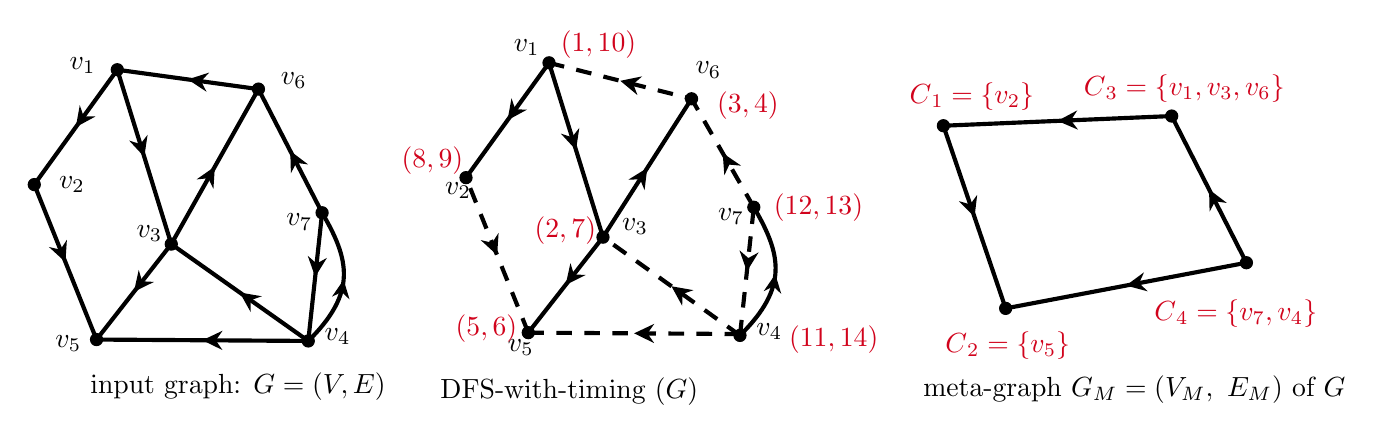
\begin{tikzpicture}[x=0.5pt,y=0.5pt,yscale=-1,xscale=1]
%uncomment if require: \path (0,284); %set diagram left start at 0, and has height of 284

%Flowchart: Connector [id:dp6832651596189389] 
\draw  [fill={rgb, 255:red, 0; green, 0; blue, 0 }  ,fill opacity=1 ] (69,40) .. controls (69,37.58) and (70.96,35.62) .. (73.38,35.62) .. controls (75.79,35.62) and (77.75,37.58) .. (77.75,40) .. controls (77.75,42.42) and (75.79,44.38) .. (73.38,44.38) .. controls (70.96,44.38) and (69,42.42) .. (69,40) -- cycle ;
%Flowchart: Connector [id:dp988004110095194] 
\draw  [fill={rgb, 255:red, 0; green, 0; blue, 0 }  ,fill opacity=1 ] (171,54) .. controls (171,51.58) and (172.96,49.62) .. (175.38,49.62) .. controls (177.79,49.62) and (179.75,51.58) .. (179.75,54) .. controls (179.75,56.42) and (177.79,58.38) .. (175.38,58.38) .. controls (172.96,58.38) and (171,56.42) .. (171,54) -- cycle ;
%Flowchart: Connector [id:dp8337455886193567] 
\draw  [fill={rgb, 255:red, 0; green, 0; blue, 0 }  ,fill opacity=1 ] (54,235) .. controls (54,232.58) and (55.96,230.62) .. (58.38,230.62) .. controls (60.79,230.62) and (62.75,232.58) .. (62.75,235) .. controls (62.75,237.42) and (60.79,239.38) .. (58.38,239.38) .. controls (55.96,239.38) and (54,237.42) .. (54,235) -- cycle ;
%Flowchart: Connector [id:dp7811656748056538] 
\draw  [fill={rgb, 255:red, 0; green, 0; blue, 0 }  ,fill opacity=1 ] (9,123) .. controls (9,120.58) and (10.96,118.62) .. (13.38,118.62) .. controls (15.79,118.62) and (17.75,120.58) .. (17.75,123) .. controls (17.75,125.42) and (15.79,127.38) .. (13.38,127.38) .. controls (10.96,127.38) and (9,125.42) .. (9,123) -- cycle ;
%Flowchart: Connector [id:dp7718177083818322] 
\draw  [fill={rgb, 255:red, 0; green, 0; blue, 0 }  ,fill opacity=1 ] (108,166) .. controls (108,163.58) and (109.96,161.62) .. (112.38,161.62) .. controls (114.79,161.62) and (116.75,163.58) .. (116.75,166) .. controls (116.75,168.42) and (114.79,170.38) .. (112.38,170.38) .. controls (109.96,170.38) and (108,168.42) .. (108,166) -- cycle ;
%Straight Lines [id:da8695282378045819] 
\draw [color={rgb, 255:red, 0; green, 0; blue, 0 }  ,draw opacity=1 ][line width=1.5]    (13.38,123) -- (73.38,40) ;
\draw [shift={(43.38,81.5)}, rotate = 305.86] [fill={rgb, 255:red, 0; green, 0; blue, 0 }  ,fill opacity=1 ][line width=0.08]  [draw opacity=0] (14.56,-6.99) -- (0,0) -- (14.56,6.99) -- (9.67,0) -- cycle    ;
%Straight Lines [id:da6240808629687105] 
\draw [color={rgb, 255:red, 0; green, 0; blue, 0 }  ,draw opacity=1 ][line width=1.5]    (58.38,235) -- (112.38,166) ;
\draw [shift={(85.38,200.5)}, rotate = 308.05] [fill={rgb, 255:red, 0; green, 0; blue, 0 }  ,fill opacity=1 ][line width=0.08]  [draw opacity=0] (14.56,-6.99) -- (0,0) -- (14.56,6.99) -- (9.67,0) -- cycle    ;
%Straight Lines [id:da28647521139148635] 
\draw [color={rgb, 255:red, 0; green, 0; blue, 0 }  ,draw opacity=1 ][line width=1.5]    (112.38,166) -- (73.38,40) ;
\draw [shift={(92.88,103)}, rotate = 252.8] [fill={rgb, 255:red, 0; green, 0; blue, 0 }  ,fill opacity=1 ][line width=0.08]  [draw opacity=0] (14.56,-6.99) -- (0,0) -- (14.56,6.99) -- (9.67,0) -- cycle    ;
%Straight Lines [id:da812435735905686] 
\draw [color={rgb, 255:red, 0; green, 0; blue, 0 }  ,draw opacity=1 ][line width=1.5]    (58.38,235) -- (13.38,123) ;
\draw [shift={(35.88,179)}, rotate = 248.11] [fill={rgb, 255:red, 0; green, 0; blue, 0 }  ,fill opacity=1 ][line width=0.08]  [draw opacity=0] (14.56,-6.99) -- (0,0) -- (14.56,6.99) -- (9.67,0) -- cycle    ;
%Flowchart: Connector [id:dp7779596833842585] 
\draw  [fill={rgb, 255:red, 0; green, 0; blue, 0 }  ,fill opacity=1 ] (207,236) .. controls (207,233.58) and (208.96,231.62) .. (211.38,231.62) .. controls (213.79,231.62) and (215.75,233.58) .. (215.75,236) .. controls (215.75,238.42) and (213.79,240.38) .. (211.38,240.38) .. controls (208.96,240.38) and (207,238.42) .. (207,236) -- cycle ;
%Straight Lines [id:da5661346124899681] 
\draw [color={rgb, 255:red, 0; green, 0; blue, 0 }  ,draw opacity=1 ][line width=1.5]    (211.38,236) -- (112.38,166) ;
\draw [shift={(161.88,201)}, rotate = 395.26] [fill={rgb, 255:red, 0; green, 0; blue, 0 }  ,fill opacity=1 ][line width=0.08]  [draw opacity=0] (14.56,-6.99) -- (0,0) -- (14.56,6.99) -- (9.67,0) -- cycle    ;
%Straight Lines [id:da9652070356210863] 
\draw [color={rgb, 255:red, 0; green, 0; blue, 0 }  ,draw opacity=1 ][line width=1.5]    (58.38,235) -- (211.38,236) ;
\draw [shift={(134.88,235.5)}, rotate = 0.37] [fill={rgb, 255:red, 0; green, 0; blue, 0 }  ,fill opacity=1 ][line width=0.08]  [draw opacity=0] (14.56,-6.99) -- (0,0) -- (14.56,6.99) -- (9.67,0) -- cycle    ;
%Flowchart: Connector [id:dp27050103826240035] 
\draw  [fill={rgb, 255:red, 0; green, 0; blue, 0 }  ,fill opacity=1 ] (217,143.38) .. controls (217,140.96) and (218.96,139) .. (221.38,139) .. controls (223.79,139) and (225.75,140.96) .. (225.75,143.38) .. controls (225.75,145.79) and (223.79,147.75) .. (221.38,147.75) .. controls (218.96,147.75) and (217,145.79) .. (217,143.38) -- cycle ;
%Straight Lines [id:da42141438650125873] 
\draw [color={rgb, 255:red, 0; green, 0; blue, 0 }  ,draw opacity=1 ][line width=1.5]    (221.38,143.38) -- (175.38,54) ;
\draw [shift={(198.38,98.69)}, rotate = 422.77] [fill={rgb, 255:red, 0; green, 0; blue, 0 }  ,fill opacity=1 ][line width=0.08]  [draw opacity=0] (14.56,-6.99) -- (0,0) -- (14.56,6.99) -- (9.67,0) -- cycle    ;
%Flowchart: Connector [id:dp9280107639837872] 
\draw  [fill={rgb, 255:red, 0; green, 0; blue, 0 }  ,fill opacity=1 ] (381,35) .. controls (381,32.58) and (382.96,30.62) .. (385.38,30.62) .. controls (387.79,30.62) and (389.75,32.58) .. (389.75,35) .. controls (389.75,37.42) and (387.79,39.38) .. (385.38,39.38) .. controls (382.96,39.38) and (381,37.42) .. (381,35) -- cycle ;
%Flowchart: Connector [id:dp32325565860173133] 
\draw  [fill={rgb, 255:red, 0; green, 0; blue, 0 }  ,fill opacity=1 ] (366,230) .. controls (366,227.58) and (367.96,225.62) .. (370.38,225.62) .. controls (372.79,225.62) and (374.75,227.58) .. (374.75,230) .. controls (374.75,232.42) and (372.79,234.38) .. (370.38,234.38) .. controls (367.96,234.38) and (366,232.42) .. (366,230) -- cycle ;
%Flowchart: Connector [id:dp9891123981062072] 
\draw  [fill={rgb, 255:red, 0; green, 0; blue, 0 }  ,fill opacity=1 ] (321,118) .. controls (321,115.58) and (322.96,113.62) .. (325.38,113.62) .. controls (327.79,113.62) and (329.75,115.58) .. (329.75,118) .. controls (329.75,120.42) and (327.79,122.38) .. (325.38,122.38) .. controls (322.96,122.38) and (321,120.42) .. (321,118) -- cycle ;
%Flowchart: Connector [id:dp40112220553719025] 
\draw  [fill={rgb, 255:red, 0; green, 0; blue, 0 }  ,fill opacity=1 ] (420,161) .. controls (420,158.58) and (421.96,156.62) .. (424.38,156.62) .. controls (426.79,156.62) and (428.75,158.58) .. (428.75,161) .. controls (428.75,163.42) and (426.79,165.38) .. (424.38,165.38) .. controls (421.96,165.38) and (420,163.42) .. (420,161) -- cycle ;
%Straight Lines [id:da23221470279057188] 
\draw [color={rgb, 255:red, 0; green, 0; blue, 0 }  ,draw opacity=1 ][line width=1.5]    (325.38,118) -- (385.38,35) ;
\draw [shift={(355.38,76.5)}, rotate = 305.86] [fill={rgb, 255:red, 0; green, 0; blue, 0 }  ,fill opacity=1 ][line width=0.08]  [draw opacity=0] (14.56,-6.99) -- (0,0) -- (14.56,6.99) -- (9.67,0) -- cycle    ;
%Straight Lines [id:da9690767143154184] 
\draw [color={rgb, 255:red, 0; green, 0; blue, 0 }  ,draw opacity=1 ][line width=1.5]  [dash pattern={on 5.63pt off 4.5pt}]  (370.38,230) -- (325.38,118) ;
\draw [shift={(347.88,174)}, rotate = 248.11] [fill={rgb, 255:red, 0; green, 0; blue, 0 }  ,fill opacity=1 ][line width=0.08]  [draw opacity=0] (14.56,-6.99) -- (0,0) -- (14.56,6.99) -- (9.67,0) -- cycle    ;
%Straight Lines [id:da5442772122834477] 
\draw [color={rgb, 255:red, 0; green, 0; blue, 0 }  ,draw opacity=1 ][line width=1.5]    (112.38,166) -- (175.38,54) ;
\draw [shift={(143.88,110)}, rotate = 479.36] [fill={rgb, 255:red, 0; green, 0; blue, 0 }  ,fill opacity=1 ][line width=0.08]  [draw opacity=0] (14.56,-6.99) -- (0,0) -- (14.56,6.99) -- (9.67,0) -- cycle    ;
%Straight Lines [id:da054951132315465334] 
\draw [color={rgb, 255:red, 0; green, 0; blue, 0 }  ,draw opacity=1 ][line width=1.5]    (73.38,40) -- (175.38,54) ;
\draw [shift={(124.38,47)}, rotate = 7.82] [fill={rgb, 255:red, 0; green, 0; blue, 0 }  ,fill opacity=1 ][line width=0.08]  [draw opacity=0] (14.56,-6.99) -- (0,0) -- (14.56,6.99) -- (9.67,0) -- cycle    ;
%Straight Lines [id:da4714865771303105] 
\draw [color={rgb, 255:red, 0; green, 0; blue, 0 }  ,draw opacity=1 ][line width=1.5]    (211.38,236) -- (221.38,143.38) ;
\draw [shift={(216.38,189.69)}, rotate = 276.16] [fill={rgb, 255:red, 0; green, 0; blue, 0 }  ,fill opacity=1 ][line width=0.08]  [draw opacity=0] (14.56,-6.99) -- (0,0) -- (14.56,6.99) -- (9.67,0) -- cycle    ;
%Flowchart: Connector [id:dp8072873078420509] 
\draw  [fill={rgb, 255:red, 0; green, 0; blue, 0 }  ,fill opacity=1 ] (484,61) .. controls (484,58.58) and (485.96,56.62) .. (488.38,56.62) .. controls (490.79,56.62) and (492.75,58.58) .. (492.75,61) .. controls (492.75,63.42) and (490.79,65.38) .. (488.38,65.38) .. controls (485.96,65.38) and (484,63.42) .. (484,61) -- cycle ;
%Straight Lines [id:da8862996829120494] 
\draw [color={rgb, 255:red, 0; green, 0; blue, 0 }  ,draw opacity=1 ][line width=1.5]    (424.38,161) -- (385.38,35) ;
\draw [shift={(404.88,98)}, rotate = 252.8] [fill={rgb, 255:red, 0; green, 0; blue, 0 }  ,fill opacity=1 ][line width=0.08]  [draw opacity=0] (14.56,-6.99) -- (0,0) -- (14.56,6.99) -- (9.67,0) -- cycle    ;
%Straight Lines [id:da8175209497677637] 
\draw [color={rgb, 255:red, 0; green, 0; blue, 0 }  ,draw opacity=1 ][line width=1.5]    (370.38,230) -- (424.38,161) ;
\draw [shift={(397.38,195.5)}, rotate = 308.05] [fill={rgb, 255:red, 0; green, 0; blue, 0 }  ,fill opacity=1 ][line width=0.08]  [draw opacity=0] (14.56,-6.99) -- (0,0) -- (14.56,6.99) -- (9.67,0) -- cycle    ;
%Straight Lines [id:da4545876322404935] 
\draw [color={rgb, 255:red, 0; green, 0; blue, 0 }  ,draw opacity=1 ][line width=1.5]    (488.38,61) -- (424.38,161) ;
\draw [shift={(456.38,111)}, rotate = 122.62] [fill={rgb, 255:red, 0; green, 0; blue, 0 }  ,fill opacity=1 ][line width=0.08]  [draw opacity=0] (14.56,-6.99) -- (0,0) -- (14.56,6.99) -- (9.67,0) -- cycle    ;
%Straight Lines [id:da2228311257049178] 
\draw [color={rgb, 255:red, 0; green, 0; blue, 0 }  ,draw opacity=1 ][line width=1.5]  [dash pattern={on 5.63pt off 4.5pt}]  (385.38,35) -- (488.38,61) ;
\draw [shift={(436.88,48)}, rotate = 14.17] [fill={rgb, 255:red, 0; green, 0; blue, 0 }  ,fill opacity=1 ][line width=0.08]  [draw opacity=0] (14.56,-6.99) -- (0,0) -- (14.56,6.99) -- (9.67,0) -- cycle    ;
%Flowchart: Connector [id:dp13927282273128694] 
\draw  [fill={rgb, 255:red, 0; green, 0; blue, 0 }  ,fill opacity=1 ] (519,232) .. controls (519,229.58) and (520.96,227.62) .. (523.38,227.62) .. controls (525.79,227.62) and (527.75,229.58) .. (527.75,232) .. controls (527.75,234.42) and (525.79,236.38) .. (523.38,236.38) .. controls (520.96,236.38) and (519,234.42) .. (519,232) -- cycle ;
%Straight Lines [id:da9522823837992999] 
\draw [color={rgb, 255:red, 0; green, 0; blue, 0 }  ,draw opacity=1 ][line width=1.5]  [dash pattern={on 5.63pt off 4.5pt}]  (523.38,232) -- (424.38,161) ;
\draw [shift={(473.88,196.5)}, rotate = 395.65] [fill={rgb, 255:red, 0; green, 0; blue, 0 }  ,fill opacity=1 ][line width=0.08]  [draw opacity=0] (14.56,-6.99) -- (0,0) -- (14.56,6.99) -- (9.67,0) -- cycle    ;
%Straight Lines [id:da9451785250835093] 
\draw [color={rgb, 255:red, 0; green, 0; blue, 0 }  ,draw opacity=1 ][line width=1.5]  [dash pattern={on 5.63pt off 4.5pt}]  (370.38,230) -- (523.38,231) ;
\draw [shift={(446.88,230.5)}, rotate = 0.37] [fill={rgb, 255:red, 0; green, 0; blue, 0 }  ,fill opacity=1 ][line width=0.08]  [draw opacity=0] (14.56,-6.99) -- (0,0) -- (14.56,6.99) -- (9.67,0) -- cycle    ;
%Flowchart: Connector [id:dp6205422729267549] 
\draw  [fill={rgb, 255:red, 0; green, 0; blue, 0 }  ,fill opacity=1 ] (529,139.38) .. controls (529,136.96) and (530.96,135) .. (533.38,135) .. controls (535.79,135) and (537.75,136.96) .. (537.75,139.38) .. controls (537.75,141.79) and (535.79,143.75) .. (533.38,143.75) .. controls (530.96,143.75) and (529,141.79) .. (529,139.38) -- cycle ;
%Straight Lines [id:da8040330863088329] 
\draw [color={rgb, 255:red, 0; green, 0; blue, 0 }  ,draw opacity=1 ][line width=1.5]  [dash pattern={on 5.63pt off 4.5pt}]  (533.38,139.38) -- (488.38,61) ;
\draw [shift={(510.88,100.19)}, rotate = 420.14] [fill={rgb, 255:red, 0; green, 0; blue, 0 }  ,fill opacity=1 ][line width=0.08]  [draw opacity=0] (14.56,-6.99) -- (0,0) -- (14.56,6.99) -- (9.67,0) -- cycle    ;
%Straight Lines [id:da270721811462559] 
\draw [color={rgb, 255:red, 0; green, 0; blue, 0 }  ,draw opacity=1 ][line width=1.5]  [dash pattern={on 5.63pt off 4.5pt}]  (523.38,232) -- (533.38,139.38) ;
\draw [shift={(528.38,185.69)}, rotate = 276.16] [fill={rgb, 255:red, 0; green, 0; blue, 0 }  ,fill opacity=1 ][line width=0.08]  [draw opacity=0] (14.56,-6.99) -- (0,0) -- (14.56,6.99) -- (9.67,0) -- cycle    ;
%Curve Lines [id:da3335117221128735] 
\draw [line width=1.5]    (211.38,236) .. controls (247,201) and (241,177) .. (221.38,143.38) ;
\draw [shift={(236.93,191.8)}, rotate = 458.86] [fill={rgb, 255:red, 0; green, 0; blue, 0 }  ][line width=0.08]  [draw opacity=0] (13.4,-6.43) -- (0,0) -- (13.4,6.44) -- (8.9,0) -- cycle    ;
%Curve Lines [id:da3048800924799854] 
\draw [line width=1.5]    (523.38,232) .. controls (559,197) and (553,173) .. (533.38,139.38) ;
\draw [shift={(548.93,187.8)}, rotate = 458.86] [fill={rgb, 255:red, 0; green, 0; blue, 0 }  ][line width=0.08]  [draw opacity=0] (13.4,-6.43) -- (0,0) -- (13.4,6.44) -- (8.9,0) -- cycle    ;
%Flowchart: Connector [id:dp4802213327188575] 
\draw  [fill={rgb, 255:red, 0; green, 0; blue, 0 }  ,fill opacity=1 ] (711,212.47) .. controls (711,210.05) and (712.96,208.09) .. (715.38,208.09) .. controls (717.79,208.09) and (719.75,210.05) .. (719.75,212.47) .. controls (719.75,214.89) and (717.79,216.85) .. (715.38,216.85) .. controls (712.96,216.85) and (711,214.89) .. (711,212.47) -- cycle ;
%Straight Lines [id:da4012018667347226] 
\draw [color={rgb, 255:red, 0; green, 0; blue, 0 }  ,draw opacity=1 ][line width=1.5]    (889.38,179.47) -- (835.38,73.47) ;
\draw [shift={(862.38,126.47)}, rotate = 423] [fill={rgb, 255:red, 0; green, 0; blue, 0 }  ,fill opacity=1 ][line width=0.08]  [draw opacity=0] (14.56,-6.99) -- (0,0) -- (14.56,6.99) -- (9.67,0) -- cycle    ;
%Flowchart: Connector [id:dp8765246990395692] 
\draw  [fill={rgb, 255:red, 0; green, 0; blue, 0 }  ,fill opacity=1 ] (831,73.47) .. controls (831,71.05) and (832.96,69.09) .. (835.38,69.09) .. controls (837.79,69.09) and (839.75,71.05) .. (839.75,73.47) .. controls (839.75,75.89) and (837.79,77.85) .. (835.38,77.85) .. controls (832.96,77.85) and (831,75.89) .. (831,73.47) -- cycle ;
%Flowchart: Connector [id:dp16478045407286646] 
\draw  [fill={rgb, 255:red, 0; green, 0; blue, 0 }  ,fill opacity=1 ] (666,80.47) .. controls (666,78.05) and (667.96,76.09) .. (670.38,76.09) .. controls (672.79,76.09) and (674.75,78.05) .. (674.75,80.47) .. controls (674.75,82.89) and (672.79,84.85) .. (670.38,84.85) .. controls (667.96,84.85) and (666,82.89) .. (666,80.47) -- cycle ;
%Straight Lines [id:da43610676953677097] 
\draw [color={rgb, 255:red, 0; green, 0; blue, 0 }  ,draw opacity=1 ][line width=1.5]    (715.38,212.47) -- (670.38,80.47) ;
\draw [shift={(692.88,146.47)}, rotate = 251.18] [fill={rgb, 255:red, 0; green, 0; blue, 0 }  ,fill opacity=1 ][line width=0.08]  [draw opacity=0] (14.56,-6.99) -- (0,0) -- (14.56,6.99) -- (9.67,0) -- cycle    ;
%Straight Lines [id:da9496215087963258] 
\draw [color={rgb, 255:red, 0; green, 0; blue, 0 }  ,draw opacity=1 ][line width=1.5]    (670.38,80.47) -- (835.38,73.47) ;
\draw [shift={(752.88,76.97)}, rotate = 357.57] [fill={rgb, 255:red, 0; green, 0; blue, 0 }  ,fill opacity=1 ][line width=0.08]  [draw opacity=0] (14.56,-6.99) -- (0,0) -- (14.56,6.99) -- (9.67,0) -- cycle    ;
%Flowchart: Connector [id:dp3010893945707027] 
\draw  [fill={rgb, 255:red, 0; green, 0; blue, 0 }  ,fill opacity=1 ] (885,179.47) .. controls (885,177.05) and (886.96,175.09) .. (889.38,175.09) .. controls (891.79,175.09) and (893.75,177.05) .. (893.75,179.47) .. controls (893.75,181.89) and (891.79,183.85) .. (889.38,183.85) .. controls (886.96,183.85) and (885,181.89) .. (885,179.47) -- cycle ;
%Straight Lines [id:da25219897920368006] 
\draw [color={rgb, 255:red, 0; green, 0; blue, 0 }  ,draw opacity=1 ][line width=1.5]    (889.38,179.47) -- (715.38,212.47) ;
\draw [shift={(802.38,195.97)}, rotate = 349.26] [fill={rgb, 255:red, 0; green, 0; blue, 0 }  ,fill opacity=1 ][line width=0.08]  [draw opacity=0] (14.56,-6.99) -- (0,0) -- (14.56,6.99) -- (9.67,0) -- cycle    ;

% Text Node
\draw (37,29) node [anchor=north west][inner sep=0.75pt]   [align=left] {$\displaystyle v_{1}$};
% Text Node
\draw (85.38,150.38) node [anchor=north west][inner sep=0.75pt]   [align=left] {$\displaystyle v_{3}$};
% Text Node
\draw (26.75,230) node [anchor=north west][inner sep=0.75pt]   [align=left] {$\displaystyle v_{5}$};
% Text Node
\draw (221.38,225.38) node [anchor=north west][inner sep=0.75pt]   [align=left] {$\displaystyle v_{4}$};
% Text Node
\draw (29.38,115.38) node [anchor=north west][inner sep=0.75pt]   [align=left] {$\displaystyle v_{2}$};
% Text Node
\draw (189.75,40.35) node [anchor=north west][inner sep=0.75pt]   [align=left] {$\displaystyle v_{6}$};
% Text Node
\draw (193.75,142.35) node [anchor=north west][inner sep=0.75pt]   [align=left] {$\displaystyle v_{7}$};
% Text Node
\draw (52,256.93) node [anchor=north west][inner sep=0.75pt]   [align=left] {input graph: $\displaystyle G=( V,E)$};
% Text Node
\draw (358,16) node [anchor=north west][inner sep=0.75pt]   [align=left] {$\displaystyle v_{1}$};
% Text Node
\draw (436.38,145.38) node [anchor=north west][inner sep=0.75pt]   [align=left] {$\displaystyle v_{3}$};
% Text Node
\draw (353.75,233) node [anchor=north west][inner sep=0.75pt]   [align=left] {$\displaystyle v_{5}$};
% Text Node
\draw (308.38,119.38) node [anchor=north west][inner sep=0.75pt]   [align=left] {$\displaystyle v_{2}$};
% Text Node
\draw (305,260.93) node [anchor=north west][inner sep=0.75pt]   [align=left] {DFS-with-timing~$\displaystyle(G)$};
% Text Node
\draw (489.38,32.48) node [anchor=north west][inner sep=0.75pt]   [align=left] {$\displaystyle v_{6}$};
% Text Node
\draw (533.38,221.38) node [anchor=north west][inner sep=0.75pt]   [align=left] {$\displaystyle v_{4}$};
% Text Node
\draw (505.75,138.35) node [anchor=north west][inner sep=0.75pt]   [align=left] {$\displaystyle v_{7}$};
% Text Node
\draw (392,10) node [anchor=north west][inner sep=0.75pt]   [align=left] {$\displaystyle \textcolor[rgb]{0.82,0.01,0.11}{(}\textcolor[rgb]{0.82,0.01,0.11}{1,10}\textcolor[rgb]{0.82,0.01,0.11}{)}$};
% Text Node
\draw (277,94) node [anchor=north west][inner sep=0.75pt]   [align=left] {$\displaystyle \textcolor[rgb]{0.82,0.01,0.11}{(}\textcolor[rgb]{0.82,0.01,0.11}{8,9}\textcolor[rgb]{0.82,0.01,0.11}{)}$};
% Text Node
\draw (316,215) node [anchor=north west][inner sep=0.75pt]   [align=left] {$\displaystyle \textcolor[rgb]{0.82,0.01,0.11}{(}\textcolor[rgb]{0.82,0.01,0.11}{5,6}\textcolor[rgb]{0.82,0.01,0.11}{)}$};
% Text Node
\draw (373,144) node [anchor=north west][inner sep=0.75pt]   [align=left] {$\displaystyle \textcolor[rgb]{0.82,0.01,0.11}{(}\textcolor[rgb]{0.82,0.01,0.11}{2,7}\textcolor[rgb]{0.82,0.01,0.11}{)}$};
% Text Node
\draw (546,128) node [anchor=north west][inner sep=0.75pt]   [align=left] {$\displaystyle \textcolor[rgb]{0.82,0.01,0.11}{(}\textcolor[rgb]{0.82,0.01,0.11}{12,13}\textcolor[rgb]{0.82,0.01,0.11}{)}$};
% Text Node
\draw (505,54) node [anchor=north west][inner sep=0.75pt]   [align=left] {$\displaystyle \textcolor[rgb]{0.82,0.01,0.11}{(}\textcolor[rgb]{0.82,0.01,0.11}{3,4}\textcolor[rgb]{0.82,0.01,0.11}{)}$};
% Text Node
\draw (557,223) node [anchor=north west][inner sep=0.75pt]   [align=left] {$\displaystyle \textcolor[rgb]{0.82,0.01,0.11}{(}\textcolor[rgb]{0.82,0.01,0.11}{11,14}\textcolor[rgb]{0.82,0.01,0.11}{)}$};
% Text Node
\draw (670,227.47) node [anchor=north west][inner sep=0.75pt]   [align=left] {$\displaystyle \textcolor[rgb]{0.82,0.01,0.11}{C}\textcolor[rgb]{0.82,0.01,0.11}{_{2} =\{v_{5}\}}$};
% Text Node
\draw (821,204.47) node [anchor=north west][inner sep=0.75pt]   [align=left] {$\displaystyle \textcolor[rgb]{0.82,0.01,0.11}{C}\textcolor[rgb]{0.82,0.01,0.11}{_{4} =\{v_{7} ,v_{4}\}}$};
% Text Node
\draw (644,47.47) node [anchor=north west][inner sep=0.75pt]   [align=left] {$\displaystyle \textcolor[rgb]{0.82,0.01,0.11}{C}\textcolor[rgb]{0.82,0.01,0.11}{_{1} =\{v_{2}\}}$};
% Text Node
\draw (770,41.47) node [anchor=north west][inner sep=0.75pt]   [align=left] {$\displaystyle \textcolor[rgb]{0.82,0.01,0.11}{C}\textcolor[rgb]{0.82,0.01,0.11}{_{3} =\{v_{1} ,v_{3} ,v_{6}\}}$};
% Text Node
\draw (654,259.47) node [anchor=north west][inner sep=0.75pt]   [align=left] {meta-graph $\displaystyle G_{M} =( V_{M} ,\ E_{M})$ of $\displaystyle G$};


\end{tikzpicture}

}
\caption{Example of running DFS~(with timing) on a directed graph. The $[pre,post]$ interval for each vertex
is marked next to each vertex.  The $postlist$ for this run is \textcolor{blue}{$postlist = (v_4,v_7,v_1,v_2,v_3,v_5,v_6)$}.  }
\label{fig:dfs}
\end{figure}



\emph{Proof.} Let $u^* := \arg\min_{u\in C_i\cup C_j} pre[u]$, i.e., $u^*$ is the first explored vertex in $C_i\cup C_j$.
Consider the two cases. 

\begin{figure}[h!]
\centering{

\tikzset{every picture/.style={line width=0.75pt}} %set default line width to 0.75pt        

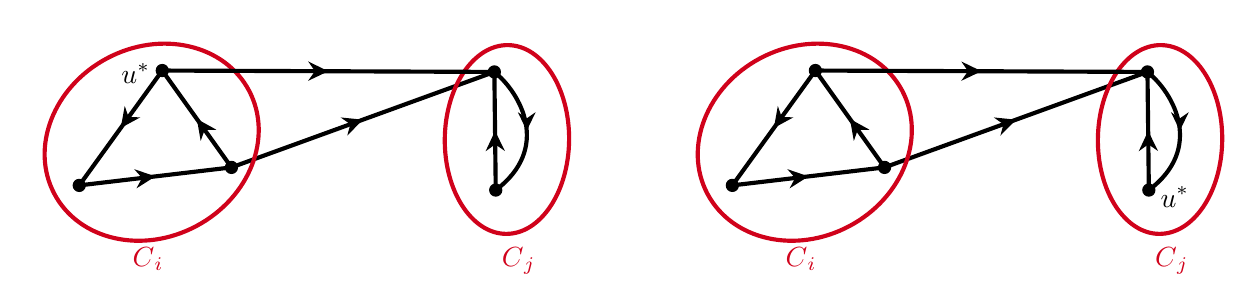
\begin{tikzpicture}[x=0.5pt,y=0.5pt,yscale=-1,xscale=1]
%uncomment if require: \path (0,196); %set diagram left start at 0, and has height of 196

%Flowchart: Connector [id:dp6536711043457765] 
\draw  [fill={rgb, 255:red, 0; green, 0; blue, 0 }  ,fill opacity=1 ] (92,42) .. controls (92,39.58) and (93.96,37.62) .. (96.38,37.62) .. controls (98.79,37.62) and (100.75,39.58) .. (100.75,42) .. controls (100.75,44.42) and (98.79,46.38) .. (96.38,46.38) .. controls (93.96,46.38) and (92,44.42) .. (92,42) -- cycle ;
%Flowchart: Connector [id:dp4048504811962438] 
\draw  [fill={rgb, 255:red, 0; green, 0; blue, 0 }  ,fill opacity=1 ] (32,125) .. controls (32,122.58) and (33.96,120.62) .. (36.38,120.62) .. controls (38.79,120.62) and (40.75,122.58) .. (40.75,125) .. controls (40.75,127.42) and (38.79,129.38) .. (36.38,129.38) .. controls (33.96,129.38) and (32,127.42) .. (32,125) -- cycle ;
%Flowchart: Connector [id:dp5803674133267218] 
\draw  [fill={rgb, 255:red, 0; green, 0; blue, 0 }  ,fill opacity=1 ] (142,112) .. controls (142,109.58) and (143.96,107.62) .. (146.38,107.62) .. controls (148.79,107.62) and (150.75,109.58) .. (150.75,112) .. controls (150.75,114.42) and (148.79,116.38) .. (146.38,116.38) .. controls (143.96,116.38) and (142,114.42) .. (142,112) -- cycle ;
%Straight Lines [id:da41352412753482715] 
\draw [color={rgb, 255:red, 0; green, 0; blue, 0 }  ,draw opacity=1 ][line width=1.5]    (36.38,125) -- (96.38,42) ;
\draw [shift={(66.38,83.5)}, rotate = 305.86] [fill={rgb, 255:red, 0; green, 0; blue, 0 }  ,fill opacity=1 ][line width=0.08]  [draw opacity=0] (14.56,-6.99) -- (0,0) -- (14.56,6.99) -- (9.67,0) -- cycle    ;
%Straight Lines [id:da10247422093058312] 
\draw [color={rgb, 255:red, 0; green, 0; blue, 0 }  ,draw opacity=1 ][line width=1.5]    (146.38,112) -- (36.38,125) ;
\draw [shift={(91.38,118.5)}, rotate = 173.26] [fill={rgb, 255:red, 0; green, 0; blue, 0 }  ,fill opacity=1 ][line width=0.08]  [draw opacity=0] (14.56,-6.99) -- (0,0) -- (14.56,6.99) -- (9.67,0) -- cycle    ;
%Flowchart: Connector [id:dp9895082549389806] 
\draw  [fill={rgb, 255:red, 0; green, 0; blue, 0 }  ,fill opacity=1 ] (333,128.38) .. controls (333,125.96) and (334.96,124) .. (337.38,124) .. controls (339.79,124) and (341.75,125.96) .. (341.75,128.38) .. controls (341.75,130.79) and (339.79,132.75) .. (337.38,132.75) .. controls (334.96,132.75) and (333,130.79) .. (333,128.38) -- cycle ;
%Straight Lines [id:da8137901366298937] 
\draw [color={rgb, 255:red, 0; green, 0; blue, 0 }  ,draw opacity=1 ][line width=1.5]    (337.38,128.38) -- (336.38,43) ;
\draw [shift={(336.88,85.69)}, rotate = 449.33] [fill={rgb, 255:red, 0; green, 0; blue, 0 }  ,fill opacity=1 ][line width=0.08]  [draw opacity=0] (14.56,-6.99) -- (0,0) -- (14.56,6.99) -- (9.67,0) -- cycle    ;
%Straight Lines [id:da15716373425720087] 
\draw [color={rgb, 255:red, 0; green, 0; blue, 0 }  ,draw opacity=1 ][line width=1.5]    (96.38,42) -- (146.38,112) ;
\draw [shift={(121.38,77)}, rotate = 54.46] [fill={rgb, 255:red, 0; green, 0; blue, 0 }  ,fill opacity=1 ][line width=0.08]  [draw opacity=0] (14.56,-6.99) -- (0,0) -- (14.56,6.99) -- (9.67,0) -- cycle    ;
%Flowchart: Connector [id:dp2761717414077073] 
\draw  [fill={rgb, 255:red, 0; green, 0; blue, 0 }  ,fill opacity=1 ] (332,43) .. controls (332,40.58) and (333.96,38.62) .. (336.38,38.62) .. controls (338.79,38.62) and (340.75,40.58) .. (340.75,43) .. controls (340.75,45.42) and (338.79,47.38) .. (336.38,47.38) .. controls (333.96,47.38) and (332,45.42) .. (332,43) -- cycle ;
%Curve Lines [id:da7005340985732622] 
\draw [line width=1.5]    (337.38,128.38) .. controls (377.38,98.38) and (355.68,58.52) .. (336.38,43) ;
\draw [shift={(359.77,85.48)}, rotate = 270.05] [fill={rgb, 255:red, 0; green, 0; blue, 0 }  ][line width=0.08]  [draw opacity=0] (13.4,-6.43) -- (0,0) -- (13.4,6.44) -- (8.9,0) -- cycle    ;
%Straight Lines [id:da9578319160914094] 
\draw [color={rgb, 255:red, 0; green, 0; blue, 0 }  ,draw opacity=1 ][line width=1.5]    (146.38,112) -- (336.38,43) ;
\draw [shift={(241.38,77.5)}, rotate = 520.04] [fill={rgb, 255:red, 0; green, 0; blue, 0 }  ,fill opacity=1 ][line width=0.08]  [draw opacity=0] (14.56,-6.99) -- (0,0) -- (14.56,6.99) -- (9.67,0) -- cycle    ;
%Shape: Ellipse [id:dp7130795758017592] 
\draw  [color={rgb, 255:red, 208; green, 2; blue, 27 }  ,draw opacity=1 ][line width=1.5]  (18.39,131.12) .. controls (0.61,97.62) and (17.68,53.75) .. (56.52,33.13) .. controls (95.37,12.52) and (141.27,22.96) .. (159.05,56.45) .. controls (176.83,89.95) and (159.76,133.82) .. (120.91,154.44) .. controls (82.07,175.06) and (36.17,164.61) .. (18.39,131.12) -- cycle ;
%Shape: Ellipse [id:dp3252588920876551] 
\draw  [color={rgb, 255:red, 208; green, 2; blue, 27 }  ,draw opacity=1 ][line width=1.5]  (346.2,23.61) .. controls (371.02,23.88) and (390.8,54.63) .. (390.4,92.31) .. controls (390,129.98) and (369.56,160.31) .. (344.75,160.04) .. controls (319.94,159.78) and (300.15,129.02) .. (300.55,91.35) .. controls (300.96,53.68) and (321.39,23.35) .. (346.2,23.61) -- cycle ;
%Straight Lines [id:da5477464737595377] 
\draw [color={rgb, 255:red, 0; green, 0; blue, 0 }  ,draw opacity=1 ][line width=1.5]    (96.38,42) -- (336.38,43) ;
\draw [shift={(216.38,42.5)}, rotate = 180.24] [fill={rgb, 255:red, 0; green, 0; blue, 0 }  ,fill opacity=1 ][line width=0.08]  [draw opacity=0] (14.56,-6.99) -- (0,0) -- (14.56,6.99) -- (9.67,0) -- cycle    ;
%Flowchart: Connector [id:dp1899602180220128] 
\draw  [fill={rgb, 255:red, 0; green, 0; blue, 0 }  ,fill opacity=1 ] (564,42) .. controls (564,39.58) and (565.96,37.62) .. (568.38,37.62) .. controls (570.79,37.62) and (572.75,39.58) .. (572.75,42) .. controls (572.75,44.42) and (570.79,46.38) .. (568.38,46.38) .. controls (565.96,46.38) and (564,44.42) .. (564,42) -- cycle ;
%Flowchart: Connector [id:dp3367645532097966] 
\draw  [fill={rgb, 255:red, 0; green, 0; blue, 0 }  ,fill opacity=1 ] (504,125) .. controls (504,122.58) and (505.96,120.62) .. (508.38,120.62) .. controls (510.79,120.62) and (512.75,122.58) .. (512.75,125) .. controls (512.75,127.42) and (510.79,129.38) .. (508.38,129.38) .. controls (505.96,129.38) and (504,127.42) .. (504,125) -- cycle ;
%Flowchart: Connector [id:dp1636605325292072] 
\draw  [fill={rgb, 255:red, 0; green, 0; blue, 0 }  ,fill opacity=1 ] (614,112) .. controls (614,109.58) and (615.96,107.62) .. (618.38,107.62) .. controls (620.79,107.62) and (622.75,109.58) .. (622.75,112) .. controls (622.75,114.42) and (620.79,116.38) .. (618.38,116.38) .. controls (615.96,116.38) and (614,114.42) .. (614,112) -- cycle ;
%Straight Lines [id:da7434793312503435] 
\draw [color={rgb, 255:red, 0; green, 0; blue, 0 }  ,draw opacity=1 ][line width=1.5]    (508.38,125) -- (568.38,42) ;
\draw [shift={(538.38,83.5)}, rotate = 305.86] [fill={rgb, 255:red, 0; green, 0; blue, 0 }  ,fill opacity=1 ][line width=0.08]  [draw opacity=0] (14.56,-6.99) -- (0,0) -- (14.56,6.99) -- (9.67,0) -- cycle    ;
%Straight Lines [id:da5706567229622709] 
\draw [color={rgb, 255:red, 0; green, 0; blue, 0 }  ,draw opacity=1 ][line width=1.5]    (618.38,112) -- (508.38,125) ;
\draw [shift={(563.38,118.5)}, rotate = 173.26] [fill={rgb, 255:red, 0; green, 0; blue, 0 }  ,fill opacity=1 ][line width=0.08]  [draw opacity=0] (14.56,-6.99) -- (0,0) -- (14.56,6.99) -- (9.67,0) -- cycle    ;
%Flowchart: Connector [id:dp05787420135544841] 
\draw  [fill={rgb, 255:red, 0; green, 0; blue, 0 }  ,fill opacity=1 ] (805,128.38) .. controls (805,125.96) and (806.96,124) .. (809.38,124) .. controls (811.79,124) and (813.75,125.96) .. (813.75,128.38) .. controls (813.75,130.79) and (811.79,132.75) .. (809.38,132.75) .. controls (806.96,132.75) and (805,130.79) .. (805,128.38) -- cycle ;
%Straight Lines [id:da9049350842223804] 
\draw [color={rgb, 255:red, 0; green, 0; blue, 0 }  ,draw opacity=1 ][line width=1.5]    (809.38,128.38) -- (808.38,43) ;
\draw [shift={(808.88,85.69)}, rotate = 449.33] [fill={rgb, 255:red, 0; green, 0; blue, 0 }  ,fill opacity=1 ][line width=0.08]  [draw opacity=0] (14.56,-6.99) -- (0,0) -- (14.56,6.99) -- (9.67,0) -- cycle    ;
%Straight Lines [id:da07605757338636099] 
\draw [color={rgb, 255:red, 0; green, 0; blue, 0 }  ,draw opacity=1 ][line width=1.5]    (568.38,42) -- (618.38,112) ;
\draw [shift={(593.38,77)}, rotate = 54.46] [fill={rgb, 255:red, 0; green, 0; blue, 0 }  ,fill opacity=1 ][line width=0.08]  [draw opacity=0] (14.56,-6.99) -- (0,0) -- (14.56,6.99) -- (9.67,0) -- cycle    ;
%Flowchart: Connector [id:dp7382748769438889] 
\draw  [fill={rgb, 255:red, 0; green, 0; blue, 0 }  ,fill opacity=1 ] (804,43) .. controls (804,40.58) and (805.96,38.62) .. (808.38,38.62) .. controls (810.79,38.62) and (812.75,40.58) .. (812.75,43) .. controls (812.75,45.42) and (810.79,47.38) .. (808.38,47.38) .. controls (805.96,47.38) and (804,45.42) .. (804,43) -- cycle ;
%Curve Lines [id:da8035156673140063] 
\draw [line width=1.5]    (809.38,128.38) .. controls (849.38,98.38) and (827.68,58.52) .. (808.38,43) ;
\draw [shift={(831.77,85.48)}, rotate = 270.05] [fill={rgb, 255:red, 0; green, 0; blue, 0 }  ][line width=0.08]  [draw opacity=0] (13.4,-6.43) -- (0,0) -- (13.4,6.44) -- (8.9,0) -- cycle    ;
%Straight Lines [id:da7412462706257437] 
\draw [color={rgb, 255:red, 0; green, 0; blue, 0 }  ,draw opacity=1 ][line width=1.5]    (618.38,112) -- (808.38,43) ;
\draw [shift={(713.38,77.5)}, rotate = 520.04] [fill={rgb, 255:red, 0; green, 0; blue, 0 }  ,fill opacity=1 ][line width=0.08]  [draw opacity=0] (14.56,-6.99) -- (0,0) -- (14.56,6.99) -- (9.67,0) -- cycle    ;
%Shape: Ellipse [id:dp18300014125728248] 
\draw  [color={rgb, 255:red, 208; green, 2; blue, 27 }  ,draw opacity=1 ][line width=1.5]  (490.39,131.12) .. controls (472.61,97.62) and (489.68,53.75) .. (528.52,33.13) .. controls (567.37,12.52) and (613.27,22.96) .. (631.05,56.45) .. controls (648.83,89.95) and (631.76,133.82) .. (592.91,154.44) .. controls (554.07,175.06) and (508.17,164.61) .. (490.39,131.12) -- cycle ;
%Shape: Ellipse [id:dp11743560021932264] 
\draw  [color={rgb, 255:red, 208; green, 2; blue, 27 }  ,draw opacity=1 ][line width=1.5]  (818.2,23.61) .. controls (843.02,23.88) and (862.8,54.63) .. (862.4,92.31) .. controls (862,129.98) and (841.56,160.31) .. (816.75,160.04) .. controls (791.94,159.78) and (772.15,129.02) .. (772.55,91.35) .. controls (772.96,53.68) and (793.39,23.35) .. (818.2,23.61) -- cycle ;
%Straight Lines [id:da4814614082608917] 
\draw [color={rgb, 255:red, 0; green, 0; blue, 0 }  ,draw opacity=1 ][line width=1.5]    (568.38,42) -- (808.38,43) ;
\draw [shift={(688.38,42.5)}, rotate = 180.24] [fill={rgb, 255:red, 0; green, 0; blue, 0 }  ,fill opacity=1 ][line width=0.08]  [draw opacity=0] (14.56,-6.99) -- (0,0) -- (14.56,6.99) -- (9.67,0) -- cycle    ;

% Text Node
\draw (65,35) node [anchor=north west][inner sep=0.75pt]   [align=left] {$\displaystyle u^{*}$};
% Text Node
\draw (73,168) node [anchor=north west][inner sep=0.75pt]   [align=left] {$\displaystyle \textcolor[rgb]{0.82,0.01,0.11}{C}\textcolor[rgb]{0.82,0.01,0.11}{_{i}}$};
% Text Node
\draw (340,168) node [anchor=north west][inner sep=0.75pt]   [align=left] {$\displaystyle \textcolor[rgb]{0.82,0.01,0.11}{C}\textcolor[rgb]{0.82,0.01,0.11}{_{j}}$};
% Text Node
\draw (816,124) node [anchor=north west][inner sep=0.75pt]   [align=left] {$\displaystyle u^{*}$};
% Text Node
\draw (545,168) node [anchor=north west][inner sep=0.75pt]   [align=left] {$\displaystyle \textcolor[rgb]{0.82,0.01,0.11}{C}\textcolor[rgb]{0.82,0.01,0.11}{_{i}}$};
% Text Node
\draw (812,168) node [anchor=north west][inner sep=0.75pt]   [align=left] {$\displaystyle \textcolor[rgb]{0.82,0.01,0.11}{C}\textcolor[rgb]{0.82,0.01,0.11}{_{j}}$};


\end{tikzpicture}

}
\caption{Two cases in proving above claim.}
\label{fig:meta}
\end{figure}

First, assume that $u^* \in C_i$. Then $u^*$ can reach all vertices in $C_i\cup C_j\setminus \{u^*\}$.
Hence, all vertices in $C_i\cup C_j\setminus \{u^*\}$ will be explored \emph{within} exploring $u^*$.
In other words, for any vertex $v\in C_i\cup C_j\setminus \{u^*\}$, the interval $[pre[v], post[v]]$
is a subset of $[pre[u^*], post[u^*]]$. This results in two facts:
$\max_{u\in C_i} post[u] = post[u^*]$ and $\max_{v\in C_j} post[v] < post[u^*]$.
Combined, we have that $\max_{u\in C_i} post[u] > \max_{v\in C_j} post[v]$.

Second, assume that $u^* \in C_j$. Then $u^*$ can \emph{not} reach any vertex in $C_i$; otherwise
$C_i\cup C_j$ form a single connected component, conflicting to the fact that any connected component must be maximal.
Hence, all vertices in $C_i$ will remain unexplored after exploring $u^*$.
In other words, for any vertex $v\in C_i$, the interval $[pre[v], post[v]]$
locates after~(and disjoint with) $[pre[u^*], post[u^*]]$. This gives that
$\max_{u\in C_i} post[u] > post[u^*]$. Besides, 
we also have $\max_{v\in C_j} post[v] = post[u^*]$ as all vertices in $C_j\setminus \{u^*\}$ will be examined within exploring $u^*$.
Combined, we have that $\max_{u\in C_i} post[u] > \max_{v\in C_j} post[v]$.
\qed

The above key claim directly suggest a property about the structure of the meta-graph, given below.

\begin{corollary}
The list of all connected components in $V_M$ sorted in decreasing order of $\max_{u\in C_i} post[u]$, $1\le i \le k$,
is a linearization of $G_M$.
\label{col1}
\end{corollary}

Verify this is the case in Figure~\ref{fig:dfs}. Answer: such list is $(C_4, C_3, C_1, C_2)$, and it is a linearization of $G_M$.

Above property also suggests us to consider an \emph{ordering of vertices} in descending post values.
Specifically, we define \emph{postlist} as such ordering of vertices.
Notice that postlist can be stored in an array and can be efficiently constructed in DFS-with-time.
Please refer to Lecture A10 for its pseudo-code.
See Figure~\ref{fig:dfs} for an example.

As a direct consequence of Corollary~\ref{col1} and the definition of postlist, we have the following property.
This is true as ``the first appearance'' exactly gives the ``largest post value'' since the postlist is sorted 
in descending order of post values.

\begin{corollary}
The list of all connected components in $V_M$
sorted by their first appearance of in the postlist is a linearization of $G_M$.
\label{col2}
\end{corollary}

Verify this is the case in Figure~\ref{fig:dfs}. Answer: following $postlist$ the corresponding list of 
connected components is $(C_4, C_4, C_3, C_1, C_3, C_2, C_3)$.
The first appearance of each component is $(C_4, C_3, C_1, C_2)$, which is a linearization of $G_M$
and exactly the one that is sorted by their largest post value.

%%
%%How about the first vertex of $postlist$? Does it in a sink vertex of $G_M$?
%%No. And Figure~\ref{fig:dfs} gives such an example: $v_6$ is the first vertex of $postlist$
%%and it is not in a sink vertex of $G_M$.
%%Note though, if $G$ is a DAG, then the first vertex of $postlist$ must be a sink of $G$,
%%as we prove that in DAGs, reverse of $postlist$ is a linearization of $G$ and the last vertex of a linearization must be a sink.

To summarize, now we can build a postlist that satisfies above Corollary~\ref{col2}.
This almost achieves the desired property of the special ordering:
``the ordering of connected components sorted by their first appearance in the
special ordering should form a reverse-linearization of the meta-graph.''
The only difference is that postlist implies a \emph{linearization} of the meta-graph
while special ordering requires a \emph{reverse-linearization} of the meta-graph.
Below, we introduce \emph{reverse graph} to fill this gap.

\subsection*{Reverse Graph}

\begin{definition}
Let $G = (V,E)$ be a directed graph. The \emph{reverse graph} of $G$, denoted as $G_R = (V, E_R)$,
has the same set of vertices and edges with reversed direction, i.e., $(u,v) \in E$ if and only if $(v,u)\in E_R$.
\end{definition}

\begin{figure}[h!]
\centering{

\tikzset{every picture/.style={line width=0.75pt}} %set default line width to 0.75pt        

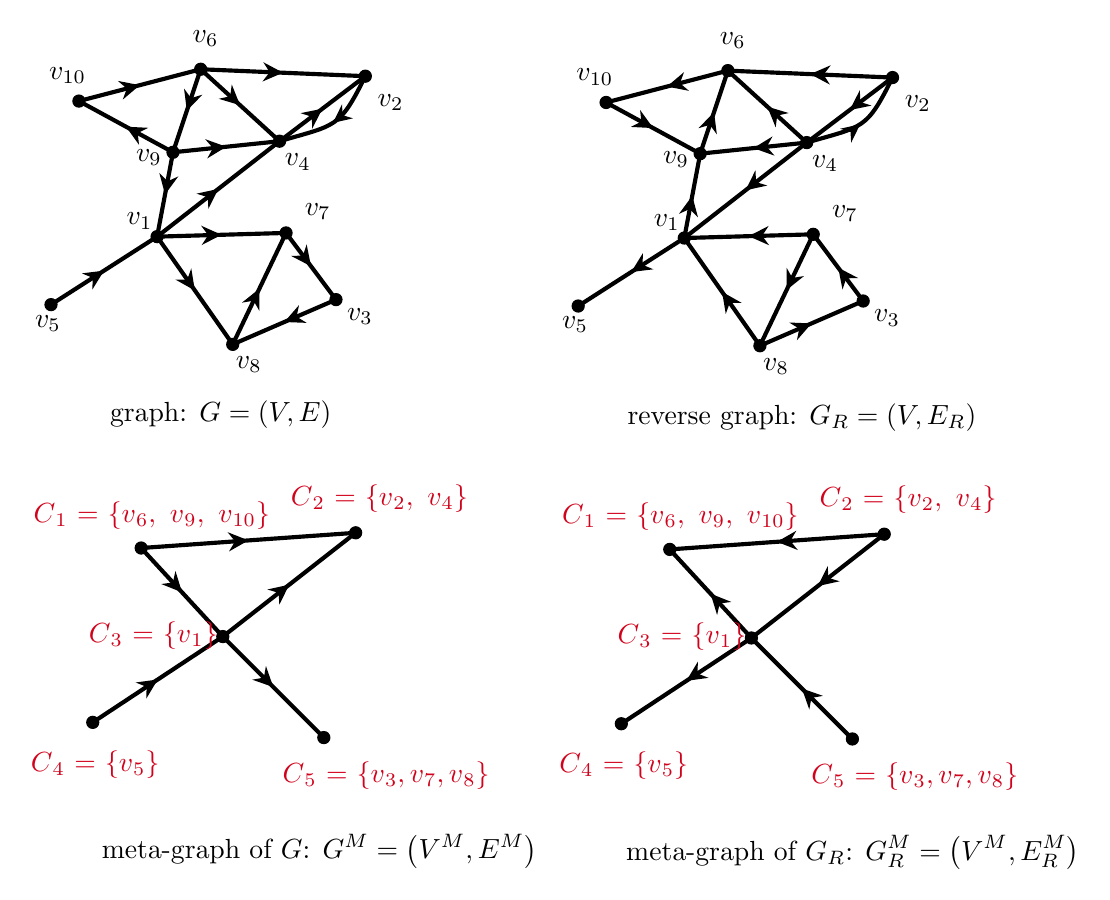
\begin{tikzpicture}[x=0.5pt,y=0.5pt,yscale=-1,xscale=1]
%uncomment if require: \path (0,615); %set diagram left start at 0, and has height of 615

%Flowchart: Connector [id:dp35531003904401826] 
\draw  [fill={rgb, 255:red, 0; green, 0; blue, 0 }  ,fill opacity=1 ] (87,378) .. controls (87,375.58) and (88.96,373.62) .. (91.38,373.62) .. controls (93.79,373.62) and (95.75,375.58) .. (95.75,378) .. controls (95.75,380.42) and (93.79,382.38) .. (91.38,382.38) .. controls (88.96,382.38) and (87,380.42) .. (87,378) -- cycle ;
%Straight Lines [id:da06413387293276729] 
\draw [color={rgb, 255:red, 0; green, 0; blue, 0 }  ,draw opacity=1 ][line width=1.5]    (114.38,92) -- (134.38,32) ;
\draw [shift={(124.38,62)}, rotate = 288.43] [fill={rgb, 255:red, 0; green, 0; blue, 0 }  ,fill opacity=1 ][line width=0.08]  [draw opacity=0] (14.56,-6.99) -- (0,0) -- (14.56,6.99) -- (9.67,0) -- cycle    ;
%Straight Lines [id:da9572573982067856] 
\draw [color={rgb, 255:red, 0; green, 0; blue, 0 }  ,draw opacity=1 ][line width=1.5]    (134.38,32) -- (46.38,55) ;
\draw [shift={(90.38,43.5)}, rotate = 165.35] [fill={rgb, 255:red, 0; green, 0; blue, 0 }  ,fill opacity=1 ][line width=0.08]  [draw opacity=0] (14.56,-6.99) -- (0,0) -- (14.56,6.99) -- (9.67,0) -- cycle    ;
%Straight Lines [id:da027017237295007268] 
\draw [color={rgb, 255:red, 0; green, 0; blue, 0 }  ,draw opacity=1 ][line width=1.5]    (150.38,442) -- (91.38,378) ;
\draw [shift={(120.88,410)}, rotate = 227.33] [fill={rgb, 255:red, 0; green, 0; blue, 0 }  ,fill opacity=1 ][line width=0.08]  [draw opacity=0] (14.56,-6.99) -- (0,0) -- (14.56,6.99) -- (9.67,0) -- cycle    ;
%Flowchart: Connector [id:dp7018202329285442] 
\draw  [fill={rgb, 255:red, 0; green, 0; blue, 0 }  ,fill opacity=1 ] (242,367) .. controls (242,364.58) and (243.96,362.62) .. (246.38,362.62) .. controls (248.79,362.62) and (250.75,364.58) .. (250.75,367) .. controls (250.75,369.42) and (248.79,371.38) .. (246.38,371.38) .. controls (243.96,371.38) and (242,369.42) .. (242,367) -- cycle ;
%Flowchart: Connector [id:dp9468304553677146] 
\draw  [fill={rgb, 255:red, 0; green, 0; blue, 0 }  ,fill opacity=1 ] (249,37) .. controls (249,34.58) and (250.96,32.62) .. (253.38,32.62) .. controls (255.79,32.62) and (257.75,34.58) .. (257.75,37) .. controls (257.75,39.42) and (255.79,41.38) .. (253.38,41.38) .. controls (250.96,41.38) and (249,39.42) .. (249,37) -- cycle ;
%Flowchart: Connector [id:dp10084257988995149] 
\draw  [fill={rgb, 255:red, 0; green, 0; blue, 0 }  ,fill opacity=1 ] (187,84) .. controls (187,81.58) and (188.96,79.62) .. (191.38,79.62) .. controls (193.79,79.62) and (195.75,81.58) .. (195.75,84) .. controls (195.75,86.42) and (193.79,88.38) .. (191.38,88.38) .. controls (188.96,88.38) and (187,86.42) .. (187,84) -- cycle ;
%Flowchart: Connector [id:dp5678652918378437] 
\draw  [fill={rgb, 255:red, 0; green, 0; blue, 0 }  ,fill opacity=1 ] (191.99,148.72) .. controls (192.85,146.46) and (195.39,145.34) .. (197.64,146.21) .. controls (199.9,147.08) and (201.02,149.61) .. (200.15,151.86) .. controls (199.28,154.12) and (196.75,155.24) .. (194.5,154.38) .. controls (192.24,153.51) and (191.12,150.97) .. (191.99,148.72) -- cycle ;
%Flowchart: Connector [id:dp9451957343710085] 
\draw  [fill={rgb, 255:red, 0; green, 0; blue, 0 }  ,fill opacity=1 ] (228.07,196.91) .. controls (228.94,194.66) and (231.47,193.53) .. (233.73,194.4) .. controls (235.98,195.27) and (237.11,197.8) .. (236.24,200.06) .. controls (235.37,202.32) and (232.84,203.44) .. (230.58,202.57) .. controls (228.33,201.7) and (227.2,199.17) .. (228.07,196.91) -- cycle ;
%Flowchart: Connector [id:dp7598246465914121] 
\draw  [fill={rgb, 255:red, 0; green, 0; blue, 0 }  ,fill opacity=1 ] (153.46,229.25) .. controls (154.33,227) and (156.86,225.87) .. (159.11,226.74) .. controls (161.37,227.61) and (162.49,230.14) .. (161.63,232.4) .. controls (160.76,234.65) and (158.22,235.78) .. (155.97,234.91) .. controls (153.71,234.04) and (152.59,231.51) .. (153.46,229.25) -- cycle ;
%Flowchart: Connector [id:dp9270593548114698] 
\draw  [fill={rgb, 255:red, 0; green, 0; blue, 0 }  ,fill opacity=1 ] (22.12,200.53) .. controls (22.99,198.28) and (25.52,197.15) .. (27.77,198.02) .. controls (30.03,198.89) and (31.15,201.42) .. (30.28,203.68) .. controls (29.42,205.94) and (26.88,207.06) .. (24.63,206.19) .. controls (22.37,205.32) and (21.25,202.79) .. (22.12,200.53) -- cycle ;
%Flowchart: Connector [id:dp0003313036349563703] 
\draw  [fill={rgb, 255:red, 0; green, 0; blue, 0 }  ,fill opacity=1 ] (98.79,151.39) .. controls (99.66,149.14) and (102.2,148.01) .. (104.45,148.88) .. controls (106.71,149.75) and (107.83,152.28) .. (106.96,154.54) .. controls (106.09,156.8) and (103.56,157.92) .. (101.3,157.05) .. controls (99.05,156.18) and (97.92,153.65) .. (98.79,151.39) -- cycle ;
%Flowchart: Connector [id:dp05524410597346219] 
\draw  [fill={rgb, 255:red, 0; green, 0; blue, 0 }  ,fill opacity=1 ] (130,32) .. controls (130,29.58) and (131.96,27.62) .. (134.38,27.62) .. controls (136.79,27.62) and (138.75,29.58) .. (138.75,32) .. controls (138.75,34.42) and (136.79,36.38) .. (134.38,36.38) .. controls (131.96,36.38) and (130,34.42) .. (130,32) -- cycle ;
%Flowchart: Connector [id:dp8722833316705884] 
\draw  [fill={rgb, 255:red, 0; green, 0; blue, 0 }  ,fill opacity=1 ] (42,55) .. controls (42,52.58) and (43.96,50.62) .. (46.38,50.62) .. controls (48.79,50.62) and (50.75,52.58) .. (50.75,55) .. controls (50.75,57.42) and (48.79,59.38) .. (46.38,59.38) .. controls (43.96,59.38) and (42,57.42) .. (42,55) -- cycle ;
%Flowchart: Connector [id:dp04902898021909796] 
\draw  [fill={rgb, 255:red, 0; green, 0; blue, 0 }  ,fill opacity=1 ] (110,92) .. controls (110,89.58) and (111.96,87.62) .. (114.38,87.62) .. controls (116.79,87.62) and (118.75,89.58) .. (118.75,92) .. controls (118.75,94.42) and (116.79,96.38) .. (114.38,96.38) .. controls (111.96,96.38) and (110,94.42) .. (110,92) -- cycle ;
%Straight Lines [id:da6957258198444844] 
\draw [color={rgb, 255:red, 0; green, 0; blue, 0 }  ,draw opacity=1 ][line width=1.5]    (46.38,55) -- (114.38,92) ;
\draw [shift={(80.38,73.5)}, rotate = 28.55] [fill={rgb, 255:red, 0; green, 0; blue, 0 }  ,fill opacity=1 ][line width=0.08]  [draw opacity=0] (14.56,-6.99) -- (0,0) -- (14.56,6.99) -- (9.67,0) -- cycle    ;
%Straight Lines [id:da1865955612168957] 
\draw [color={rgb, 255:red, 0; green, 0; blue, 0 }  ,draw opacity=1 ][line width=1.5]    (102.88,152.97) -- (114.38,92) ;
\draw [shift={(108.63,122.48)}, rotate = 280.68] [fill={rgb, 255:red, 0; green, 0; blue, 0 }  ,fill opacity=1 ][line width=0.08]  [draw opacity=0] (14.56,-6.99) -- (0,0) -- (14.56,6.99) -- (9.67,0) -- cycle    ;
%Straight Lines [id:da5983156386140572] 
\draw [color={rgb, 255:red, 0; green, 0; blue, 0 }  ,draw opacity=1 ][line width=1.5]    (102.88,152.97) -- (26.2,202.11) ;
\draw [shift={(64.54,177.54)}, rotate = 147.35] [fill={rgb, 255:red, 0; green, 0; blue, 0 }  ,fill opacity=1 ][line width=0.08]  [draw opacity=0] (14.56,-6.99) -- (0,0) -- (14.56,6.99) -- (9.67,0) -- cycle    ;
%Straight Lines [id:da7813440675788919] 
\draw [color={rgb, 255:red, 0; green, 0; blue, 0 }  ,draw opacity=1 ][line width=1.5]    (157.54,230.82) -- (102.88,152.97) ;
\draw [shift={(130.21,191.9)}, rotate = 234.93] [fill={rgb, 255:red, 0; green, 0; blue, 0 }  ,fill opacity=1 ][line width=0.08]  [draw opacity=0] (14.56,-6.99) -- (0,0) -- (14.56,6.99) -- (9.67,0) -- cycle    ;
%Straight Lines [id:da11231036470839317] 
\draw [color={rgb, 255:red, 0; green, 0; blue, 0 }  ,draw opacity=1 ][line width=1.5]    (196.07,150.29) -- (102.88,152.97) ;
\draw [shift={(149.47,151.63)}, rotate = 178.36] [fill={rgb, 255:red, 0; green, 0; blue, 0 }  ,fill opacity=1 ][line width=0.08]  [draw opacity=0] (14.56,-6.99) -- (0,0) -- (14.56,6.99) -- (9.67,0) -- cycle    ;
%Straight Lines [id:da3818914730957623] 
\draw [color={rgb, 255:red, 0; green, 0; blue, 0 }  ,draw opacity=1 ][line width=1.5]    (196.07,150.29) -- (157.54,230.82) ;
\draw [shift={(176.81,190.56)}, rotate = 115.57] [fill={rgb, 255:red, 0; green, 0; blue, 0 }  ,fill opacity=1 ][line width=0.08]  [draw opacity=0] (14.56,-6.99) -- (0,0) -- (14.56,6.99) -- (9.67,0) -- cycle    ;
%Straight Lines [id:da5617379482893489] 
\draw [color={rgb, 255:red, 0; green, 0; blue, 0 }  ,draw opacity=1 ][line width=1.5]    (157.54,230.82) -- (232.16,198.49) ;
\draw [shift={(194.85,214.66)}, rotate = 336.57] [fill={rgb, 255:red, 0; green, 0; blue, 0 }  ,fill opacity=1 ][line width=0.08]  [draw opacity=0] (14.56,-6.99) -- (0,0) -- (14.56,6.99) -- (9.67,0) -- cycle    ;
%Straight Lines [id:da7816864329937088] 
\draw [color={rgb, 255:red, 0; green, 0; blue, 0 }  ,draw opacity=1 ][line width=1.5]    (232.16,198.49) -- (196.07,150.29) ;
\draw [shift={(214.11,174.39)}, rotate = 233.18] [fill={rgb, 255:red, 0; green, 0; blue, 0 }  ,fill opacity=1 ][line width=0.08]  [draw opacity=0] (14.56,-6.99) -- (0,0) -- (14.56,6.99) -- (9.67,0) -- cycle    ;
%Straight Lines [id:da007998244336271831] 
\draw [color={rgb, 255:red, 0; green, 0; blue, 0 }  ,draw opacity=1 ][line width=1.5]    (191.38,84) -- (102.88,152.97) ;
\draw [shift={(147.13,118.48)}, rotate = 142.07] [fill={rgb, 255:red, 0; green, 0; blue, 0 }  ,fill opacity=1 ][line width=0.08]  [draw opacity=0] (14.56,-6.99) -- (0,0) -- (14.56,6.99) -- (9.67,0) -- cycle    ;
%Straight Lines [id:da07370415553910226] 
\draw [color={rgb, 255:red, 0; green, 0; blue, 0 }  ,draw opacity=1 ][line width=1.5]    (253.38,37) -- (191.38,84) ;
\draw [shift={(222.38,60.5)}, rotate = 142.84] [fill={rgb, 255:red, 0; green, 0; blue, 0 }  ,fill opacity=1 ][line width=0.08]  [draw opacity=0] (14.56,-6.99) -- (0,0) -- (14.56,6.99) -- (9.67,0) -- cycle    ;
%Straight Lines [id:da31265226854681183] 
\draw [color={rgb, 255:red, 0; green, 0; blue, 0 }  ,draw opacity=1 ][line width=1.5]    (253.38,37) -- (134.38,32) ;
\draw [shift={(193.88,34.5)}, rotate = 182.41] [fill={rgb, 255:red, 0; green, 0; blue, 0 }  ,fill opacity=1 ][line width=0.08]  [draw opacity=0] (14.56,-6.99) -- (0,0) -- (14.56,6.99) -- (9.67,0) -- cycle    ;
%Straight Lines [id:da03944598876714689] 
\draw [color={rgb, 255:red, 0; green, 0; blue, 0 }  ,draw opacity=1 ][line width=1.5]    (191.38,84) -- (114.38,92) ;
\draw [shift={(152.88,88)}, rotate = 174.07] [fill={rgb, 255:red, 0; green, 0; blue, 0 }  ,fill opacity=1 ][line width=0.08]  [draw opacity=0] (14.56,-6.99) -- (0,0) -- (14.56,6.99) -- (9.67,0) -- cycle    ;
%Curve Lines [id:da24538681443295773] 
\draw [line width=1.5]    (253.38,37) .. controls (234.5,75) and (232.5,72) .. (191.38,84) ;
\draw [shift={(229.99,70.74)}, rotate = 321.64] [fill={rgb, 255:red, 0; green, 0; blue, 0 }  ][line width=0.08]  [draw opacity=0] (13.4,-6.43) -- (0,0) -- (13.4,6.44) -- (8.9,0) -- cycle    ;
%Straight Lines [id:da5495061302418803] 
\draw [color={rgb, 255:red, 0; green, 0; blue, 0 }  ,draw opacity=1 ][line width=1.5]    (191.38,84) -- (134.38,32) ;
\draw [shift={(162.88,58)}, rotate = 222.37] [fill={rgb, 255:red, 0; green, 0; blue, 0 }  ,fill opacity=1 ][line width=0.08]  [draw opacity=0] (14.56,-6.99) -- (0,0) -- (14.56,6.99) -- (9.67,0) -- cycle    ;
%Flowchart: Connector [id:dp24932583909944328] 
\draw  [fill={rgb, 255:red, 0; green, 0; blue, 0 }  ,fill opacity=1 ] (146,442) .. controls (146,439.58) and (147.96,437.62) .. (150.38,437.62) .. controls (152.79,437.62) and (154.75,439.58) .. (154.75,442) .. controls (154.75,444.42) and (152.79,446.38) .. (150.38,446.38) .. controls (147.96,446.38) and (146,444.42) .. (146,442) -- cycle ;
%Flowchart: Connector [id:dp3666265572902413] 
\draw  [fill={rgb, 255:red, 0; green, 0; blue, 0 }  ,fill opacity=1 ] (52,504) .. controls (52,501.58) and (53.96,499.62) .. (56.38,499.62) .. controls (58.79,499.62) and (60.75,501.58) .. (60.75,504) .. controls (60.75,506.42) and (58.79,508.38) .. (56.38,508.38) .. controls (53.96,508.38) and (52,506.42) .. (52,504) -- cycle ;
%Flowchart: Connector [id:dp5809100494545972] 
\draw  [fill={rgb, 255:red, 0; green, 0; blue, 0 }  ,fill opacity=1 ] (219,515) .. controls (219,512.58) and (220.96,510.62) .. (223.38,510.62) .. controls (225.79,510.62) and (227.75,512.58) .. (227.75,515) .. controls (227.75,517.42) and (225.79,519.38) .. (223.38,519.38) .. controls (220.96,519.38) and (219,517.42) .. (219,515) -- cycle ;
%Straight Lines [id:da1229562998864333] 
\draw [color={rgb, 255:red, 0; green, 0; blue, 0 }  ,draw opacity=1 ][line width=1.5]    (246.38,367) -- (91.38,378) ;
\draw [shift={(168.88,372.5)}, rotate = 175.94] [fill={rgb, 255:red, 0; green, 0; blue, 0 }  ,fill opacity=1 ][line width=0.08]  [draw opacity=0] (14.56,-6.99) -- (0,0) -- (14.56,6.99) -- (9.67,0) -- cycle    ;
%Straight Lines [id:da6177657045500177] 
\draw [color={rgb, 255:red, 0; green, 0; blue, 0 }  ,draw opacity=1 ][line width=1.5]    (246.38,367) -- (150.38,442) ;
\draw [shift={(198.38,404.5)}, rotate = 142] [fill={rgb, 255:red, 0; green, 0; blue, 0 }  ,fill opacity=1 ][line width=0.08]  [draw opacity=0] (14.56,-6.99) -- (0,0) -- (14.56,6.99) -- (9.67,0) -- cycle    ;
%Straight Lines [id:da45439161896636415] 
\draw [color={rgb, 255:red, 0; green, 0; blue, 0 }  ,draw opacity=1 ][line width=1.5]    (223.38,515) -- (150.38,442) ;
\draw [shift={(186.88,478.5)}, rotate = 225] [fill={rgb, 255:red, 0; green, 0; blue, 0 }  ,fill opacity=1 ][line width=0.08]  [draw opacity=0] (14.56,-6.99) -- (0,0) -- (14.56,6.99) -- (9.67,0) -- cycle    ;
%Straight Lines [id:da11561285868658588] 
\draw [color={rgb, 255:red, 0; green, 0; blue, 0 }  ,draw opacity=1 ][line width=1.5]    (150.38,442) -- (56.38,504) ;
\draw [shift={(103.38,473)}, rotate = 146.59] [fill={rgb, 255:red, 0; green, 0; blue, 0 }  ,fill opacity=1 ][line width=0.08]  [draw opacity=0] (14.56,-6.99) -- (0,0) -- (14.56,6.99) -- (9.67,0) -- cycle    ;
%Straight Lines [id:da8168779159006088] 
\draw [color={rgb, 255:red, 0; green, 0; blue, 0 }  ,draw opacity=1 ][line width=1.5]    (495.38,93) -- (515.38,33) ;
\draw [shift={(505.38,63)}, rotate = 468.43] [fill={rgb, 255:red, 0; green, 0; blue, 0 }  ,fill opacity=1 ][line width=0.08]  [draw opacity=0] (14.56,-6.99) -- (0,0) -- (14.56,6.99) -- (9.67,0) -- cycle    ;
%Straight Lines [id:da894325464874] 
\draw [color={rgb, 255:red, 0; green, 0; blue, 0 }  ,draw opacity=1 ][line width=1.5]    (515.38,33) -- (427.38,56) ;
\draw [shift={(471.38,44.5)}, rotate = 345.35] [fill={rgb, 255:red, 0; green, 0; blue, 0 }  ,fill opacity=1 ][line width=0.08]  [draw opacity=0] (14.56,-6.99) -- (0,0) -- (14.56,6.99) -- (9.67,0) -- cycle    ;
%Flowchart: Connector [id:dp2028061961127232] 
\draw  [fill={rgb, 255:red, 0; green, 0; blue, 0 }  ,fill opacity=1 ] (630,38) .. controls (630,35.58) and (631.96,33.62) .. (634.38,33.62) .. controls (636.79,33.62) and (638.75,35.58) .. (638.75,38) .. controls (638.75,40.42) and (636.79,42.38) .. (634.38,42.38) .. controls (631.96,42.38) and (630,40.42) .. (630,38) -- cycle ;
%Flowchart: Connector [id:dp6685886791876837] 
\draw  [fill={rgb, 255:red, 0; green, 0; blue, 0 }  ,fill opacity=1 ] (568,85) .. controls (568,82.58) and (569.96,80.62) .. (572.38,80.62) .. controls (574.79,80.62) and (576.75,82.58) .. (576.75,85) .. controls (576.75,87.42) and (574.79,89.38) .. (572.38,89.38) .. controls (569.96,89.38) and (568,87.42) .. (568,85) -- cycle ;
%Flowchart: Connector [id:dp6828969280331417] 
\draw  [fill={rgb, 255:red, 0; green, 0; blue, 0 }  ,fill opacity=1 ] (572.99,149.72) .. controls (573.85,147.46) and (576.39,146.34) .. (578.64,147.21) .. controls (580.9,148.08) and (582.02,150.61) .. (581.15,152.86) .. controls (580.28,155.12) and (577.75,156.24) .. (575.5,155.38) .. controls (573.24,154.51) and (572.12,151.97) .. (572.99,149.72) -- cycle ;
%Flowchart: Connector [id:dp5869007902050025] 
\draw  [fill={rgb, 255:red, 0; green, 0; blue, 0 }  ,fill opacity=1 ] (609.07,197.91) .. controls (609.94,195.66) and (612.47,194.53) .. (614.73,195.4) .. controls (616.98,196.27) and (618.11,198.8) .. (617.24,201.06) .. controls (616.37,203.32) and (613.84,204.44) .. (611.58,203.57) .. controls (609.33,202.7) and (608.2,200.17) .. (609.07,197.91) -- cycle ;
%Flowchart: Connector [id:dp29745484225367824] 
\draw  [fill={rgb, 255:red, 0; green, 0; blue, 0 }  ,fill opacity=1 ] (534.46,230.25) .. controls (535.33,228) and (537.86,226.87) .. (540.11,227.74) .. controls (542.37,228.61) and (543.49,231.14) .. (542.63,233.4) .. controls (541.76,235.65) and (539.22,236.78) .. (536.97,235.91) .. controls (534.71,235.04) and (533.59,232.51) .. (534.46,230.25) -- cycle ;
%Flowchart: Connector [id:dp9007070710643801] 
\draw  [fill={rgb, 255:red, 0; green, 0; blue, 0 }  ,fill opacity=1 ] (403.12,201.53) .. controls (403.99,199.28) and (406.52,198.15) .. (408.77,199.02) .. controls (411.03,199.89) and (412.15,202.42) .. (411.28,204.68) .. controls (410.42,206.94) and (407.88,208.06) .. (405.63,207.19) .. controls (403.37,206.32) and (402.25,203.79) .. (403.12,201.53) -- cycle ;
%Flowchart: Connector [id:dp8032522319169138] 
\draw  [fill={rgb, 255:red, 0; green, 0; blue, 0 }  ,fill opacity=1 ] (479.79,152.39) .. controls (480.66,150.14) and (483.2,149.01) .. (485.45,149.88) .. controls (487.71,150.75) and (488.83,153.28) .. (487.96,155.54) .. controls (487.09,157.8) and (484.56,158.92) .. (482.3,158.05) .. controls (480.05,157.18) and (478.92,154.65) .. (479.79,152.39) -- cycle ;
%Flowchart: Connector [id:dp3269943450949304] 
\draw  [fill={rgb, 255:red, 0; green, 0; blue, 0 }  ,fill opacity=1 ] (511,33) .. controls (511,30.58) and (512.96,28.62) .. (515.38,28.62) .. controls (517.79,28.62) and (519.75,30.58) .. (519.75,33) .. controls (519.75,35.42) and (517.79,37.38) .. (515.38,37.38) .. controls (512.96,37.38) and (511,35.42) .. (511,33) -- cycle ;
%Flowchart: Connector [id:dp23422253916024505] 
\draw  [fill={rgb, 255:red, 0; green, 0; blue, 0 }  ,fill opacity=1 ] (423,56) .. controls (423,53.58) and (424.96,51.62) .. (427.38,51.62) .. controls (429.79,51.62) and (431.75,53.58) .. (431.75,56) .. controls (431.75,58.42) and (429.79,60.38) .. (427.38,60.38) .. controls (424.96,60.38) and (423,58.42) .. (423,56) -- cycle ;
%Flowchart: Connector [id:dp010586655389437372] 
\draw  [fill={rgb, 255:red, 0; green, 0; blue, 0 }  ,fill opacity=1 ] (491,93) .. controls (491,90.58) and (492.96,88.62) .. (495.38,88.62) .. controls (497.79,88.62) and (499.75,90.58) .. (499.75,93) .. controls (499.75,95.42) and (497.79,97.38) .. (495.38,97.38) .. controls (492.96,97.38) and (491,95.42) .. (491,93) -- cycle ;
%Straight Lines [id:da51057635409129] 
\draw [color={rgb, 255:red, 0; green, 0; blue, 0 }  ,draw opacity=1 ][line width=1.5]    (427.38,56) -- (495.38,93) ;
\draw [shift={(461.38,74.5)}, rotate = 208.55] [fill={rgb, 255:red, 0; green, 0; blue, 0 }  ,fill opacity=1 ][line width=0.08]  [draw opacity=0] (14.56,-6.99) -- (0,0) -- (14.56,6.99) -- (9.67,0) -- cycle    ;
%Straight Lines [id:da9705884712552635] 
\draw [color={rgb, 255:red, 0; green, 0; blue, 0 }  ,draw opacity=1 ][line width=1.5]    (483.88,153.97) -- (495.38,93) ;
\draw [shift={(489.63,123.48)}, rotate = 460.68] [fill={rgb, 255:red, 0; green, 0; blue, 0 }  ,fill opacity=1 ][line width=0.08]  [draw opacity=0] (14.56,-6.99) -- (0,0) -- (14.56,6.99) -- (9.67,0) -- cycle    ;
%Straight Lines [id:da5127893862513866] 
\draw [color={rgb, 255:red, 0; green, 0; blue, 0 }  ,draw opacity=1 ][line width=1.5]    (483.88,153.97) -- (407.2,203.11) ;
\draw [shift={(445.54,178.54)}, rotate = 327.35] [fill={rgb, 255:red, 0; green, 0; blue, 0 }  ,fill opacity=1 ][line width=0.08]  [draw opacity=0] (14.56,-6.99) -- (0,0) -- (14.56,6.99) -- (9.67,0) -- cycle    ;
%Straight Lines [id:da5716196586001995] 
\draw [color={rgb, 255:red, 0; green, 0; blue, 0 }  ,draw opacity=1 ][line width=1.5]    (538.54,231.82) -- (483.88,153.97) ;
\draw [shift={(511.21,192.9)}, rotate = 414.93] [fill={rgb, 255:red, 0; green, 0; blue, 0 }  ,fill opacity=1 ][line width=0.08]  [draw opacity=0] (14.56,-6.99) -- (0,0) -- (14.56,6.99) -- (9.67,0) -- cycle    ;
%Straight Lines [id:da9185935928544606] 
\draw [color={rgb, 255:red, 0; green, 0; blue, 0 }  ,draw opacity=1 ][line width=1.5]    (577.07,151.29) -- (483.88,153.97) ;
\draw [shift={(530.47,152.63)}, rotate = 358.36] [fill={rgb, 255:red, 0; green, 0; blue, 0 }  ,fill opacity=1 ][line width=0.08]  [draw opacity=0] (14.56,-6.99) -- (0,0) -- (14.56,6.99) -- (9.67,0) -- cycle    ;
%Straight Lines [id:da5526780501990177] 
\draw [color={rgb, 255:red, 0; green, 0; blue, 0 }  ,draw opacity=1 ][line width=1.5]    (577.07,151.29) -- (538.54,231.82) ;
\draw [shift={(557.81,191.56)}, rotate = 295.57] [fill={rgb, 255:red, 0; green, 0; blue, 0 }  ,fill opacity=1 ][line width=0.08]  [draw opacity=0] (14.56,-6.99) -- (0,0) -- (14.56,6.99) -- (9.67,0) -- cycle    ;
%Straight Lines [id:da07669648878710078] 
\draw [color={rgb, 255:red, 0; green, 0; blue, 0 }  ,draw opacity=1 ][line width=1.5]    (538.54,231.82) -- (613.16,199.49) ;
\draw [shift={(575.85,215.66)}, rotate = 516.5699999999999] [fill={rgb, 255:red, 0; green, 0; blue, 0 }  ,fill opacity=1 ][line width=0.08]  [draw opacity=0] (14.56,-6.99) -- (0,0) -- (14.56,6.99) -- (9.67,0) -- cycle    ;
%Straight Lines [id:da04407384927929969] 
\draw [color={rgb, 255:red, 0; green, 0; blue, 0 }  ,draw opacity=1 ][line width=1.5]    (613.16,199.49) -- (577.07,151.29) ;
\draw [shift={(595.11,175.39)}, rotate = 413.18] [fill={rgb, 255:red, 0; green, 0; blue, 0 }  ,fill opacity=1 ][line width=0.08]  [draw opacity=0] (14.56,-6.99) -- (0,0) -- (14.56,6.99) -- (9.67,0) -- cycle    ;
%Straight Lines [id:da7736173583087967] 
\draw [color={rgb, 255:red, 0; green, 0; blue, 0 }  ,draw opacity=1 ][line width=1.5]    (572.38,85) -- (483.88,153.97) ;
\draw [shift={(528.13,119.48)}, rotate = 322.07] [fill={rgb, 255:red, 0; green, 0; blue, 0 }  ,fill opacity=1 ][line width=0.08]  [draw opacity=0] (14.56,-6.99) -- (0,0) -- (14.56,6.99) -- (9.67,0) -- cycle    ;
%Straight Lines [id:da984046162104014] 
\draw [color={rgb, 255:red, 0; green, 0; blue, 0 }  ,draw opacity=1 ][line width=1.5]    (634.38,38) -- (572.38,85) ;
\draw [shift={(603.38,61.5)}, rotate = 322.84000000000003] [fill={rgb, 255:red, 0; green, 0; blue, 0 }  ,fill opacity=1 ][line width=0.08]  [draw opacity=0] (14.56,-6.99) -- (0,0) -- (14.56,6.99) -- (9.67,0) -- cycle    ;
%Straight Lines [id:da41303131230822765] 
\draw [color={rgb, 255:red, 0; green, 0; blue, 0 }  ,draw opacity=1 ][line width=1.5]    (634.38,38) -- (515.38,33) ;
\draw [shift={(574.88,35.5)}, rotate = 362.40999999999997] [fill={rgb, 255:red, 0; green, 0; blue, 0 }  ,fill opacity=1 ][line width=0.08]  [draw opacity=0] (14.56,-6.99) -- (0,0) -- (14.56,6.99) -- (9.67,0) -- cycle    ;
%Straight Lines [id:da9312483814272712] 
\draw [color={rgb, 255:red, 0; green, 0; blue, 0 }  ,draw opacity=1 ][line width=1.5]    (572.38,85) -- (495.38,93) ;
\draw [shift={(533.88,89)}, rotate = 354.07] [fill={rgb, 255:red, 0; green, 0; blue, 0 }  ,fill opacity=1 ][line width=0.08]  [draw opacity=0] (14.56,-6.99) -- (0,0) -- (14.56,6.99) -- (9.67,0) -- cycle    ;
%Curve Lines [id:da6657670157747444] 
\draw [line width=1.5]    (634.38,38) .. controls (615.5,76) and (613.5,73) .. (572.38,85) ;
\draw [shift={(610.99,71.74)}, rotate = 141.64] [fill={rgb, 255:red, 0; green, 0; blue, 0 }  ][line width=0.08]  [draw opacity=0] (13.4,-6.43) -- (0,0) -- (13.4,6.44) -- (8.9,0) -- cycle    ;
%Straight Lines [id:da6019953764665212] 
\draw [color={rgb, 255:red, 0; green, 0; blue, 0 }  ,draw opacity=1 ][line width=1.5]    (572.38,85) -- (515.38,33) ;
\draw [shift={(543.88,59)}, rotate = 402.37] [fill={rgb, 255:red, 0; green, 0; blue, 0 }  ,fill opacity=1 ][line width=0.08]  [draw opacity=0] (14.56,-6.99) -- (0,0) -- (14.56,6.99) -- (9.67,0) -- cycle    ;
%Flowchart: Connector [id:dp2447453141676298] 
\draw  [fill={rgb, 255:red, 0; green, 0; blue, 0 }  ,fill opacity=1 ] (469,379) .. controls (469,376.58) and (470.96,374.62) .. (473.38,374.62) .. controls (475.79,374.62) and (477.75,376.58) .. (477.75,379) .. controls (477.75,381.42) and (475.79,383.38) .. (473.38,383.38) .. controls (470.96,383.38) and (469,381.42) .. (469,379) -- cycle ;
%Straight Lines [id:da8606033691768754] 
\draw [color={rgb, 255:red, 0; green, 0; blue, 0 }  ,draw opacity=1 ][line width=1.5]    (532.38,443) -- (473.38,379) ;
\draw [shift={(502.88,411)}, rotate = 407.33000000000004] [fill={rgb, 255:red, 0; green, 0; blue, 0 }  ,fill opacity=1 ][line width=0.08]  [draw opacity=0] (14.56,-6.99) -- (0,0) -- (14.56,6.99) -- (9.67,0) -- cycle    ;
%Flowchart: Connector [id:dp591146190566066] 
\draw  [fill={rgb, 255:red, 0; green, 0; blue, 0 }  ,fill opacity=1 ] (624,368) .. controls (624,365.58) and (625.96,363.62) .. (628.38,363.62) .. controls (630.79,363.62) and (632.75,365.58) .. (632.75,368) .. controls (632.75,370.42) and (630.79,372.38) .. (628.38,372.38) .. controls (625.96,372.38) and (624,370.42) .. (624,368) -- cycle ;
%Flowchart: Connector [id:dp231499536937802] 
\draw  [fill={rgb, 255:red, 0; green, 0; blue, 0 }  ,fill opacity=1 ] (528,443) .. controls (528,440.58) and (529.96,438.62) .. (532.38,438.62) .. controls (534.79,438.62) and (536.75,440.58) .. (536.75,443) .. controls (536.75,445.42) and (534.79,447.38) .. (532.38,447.38) .. controls (529.96,447.38) and (528,445.42) .. (528,443) -- cycle ;
%Flowchart: Connector [id:dp47523679634028715] 
\draw  [fill={rgb, 255:red, 0; green, 0; blue, 0 }  ,fill opacity=1 ] (434,505) .. controls (434,502.58) and (435.96,500.62) .. (438.38,500.62) .. controls (440.79,500.62) and (442.75,502.58) .. (442.75,505) .. controls (442.75,507.42) and (440.79,509.38) .. (438.38,509.38) .. controls (435.96,509.38) and (434,507.42) .. (434,505) -- cycle ;
%Flowchart: Connector [id:dp593330998531193] 
\draw  [fill={rgb, 255:red, 0; green, 0; blue, 0 }  ,fill opacity=1 ] (601,516) .. controls (601,513.58) and (602.96,511.62) .. (605.38,511.62) .. controls (607.79,511.62) and (609.75,513.58) .. (609.75,516) .. controls (609.75,518.42) and (607.79,520.38) .. (605.38,520.38) .. controls (602.96,520.38) and (601,518.42) .. (601,516) -- cycle ;
%Straight Lines [id:da05923813499561881] 
\draw [color={rgb, 255:red, 0; green, 0; blue, 0 }  ,draw opacity=1 ][line width=1.5]    (628.38,368) -- (473.38,379) ;
\draw [shift={(550.88,373.5)}, rotate = 355.94] [fill={rgb, 255:red, 0; green, 0; blue, 0 }  ,fill opacity=1 ][line width=0.08]  [draw opacity=0] (14.56,-6.99) -- (0,0) -- (14.56,6.99) -- (9.67,0) -- cycle    ;
%Straight Lines [id:da4311696280051074] 
\draw [color={rgb, 255:red, 0; green, 0; blue, 0 }  ,draw opacity=1 ][line width=1.5]    (628.38,368) -- (532.38,443) ;
\draw [shift={(580.38,405.5)}, rotate = 322] [fill={rgb, 255:red, 0; green, 0; blue, 0 }  ,fill opacity=1 ][line width=0.08]  [draw opacity=0] (14.56,-6.99) -- (0,0) -- (14.56,6.99) -- (9.67,0) -- cycle    ;
%Straight Lines [id:da8663749303427544] 
\draw [color={rgb, 255:red, 0; green, 0; blue, 0 }  ,draw opacity=1 ][line width=1.5]    (605.38,516) -- (532.38,443) ;
\draw [shift={(568.88,479.5)}, rotate = 405] [fill={rgb, 255:red, 0; green, 0; blue, 0 }  ,fill opacity=1 ][line width=0.08]  [draw opacity=0] (14.56,-6.99) -- (0,0) -- (14.56,6.99) -- (9.67,0) -- cycle    ;
%Straight Lines [id:da34096248111738436] 
\draw [color={rgb, 255:red, 0; green, 0; blue, 0 }  ,draw opacity=1 ][line width=1.5]    (532.38,443) -- (438.38,505) ;
\draw [shift={(485.38,474)}, rotate = 326.59000000000003] [fill={rgb, 255:red, 0; green, 0; blue, 0 }  ,fill opacity=1 ][line width=0.08]  [draw opacity=0] (14.56,-6.99) -- (0,0) -- (14.56,6.99) -- (9.67,0) -- cycle    ;

% Text Node
\draw (79,134) node [anchor=north west][inner sep=0.75pt]   [align=left] {$\displaystyle v_{1}$};
% Text Node
\draw (238.24,203.06) node [anchor=north west][inner sep=0.75pt]   [align=left] {$\displaystyle v_{3}$};
% Text Node
\draw (12.75,208) node [anchor=north west][inner sep=0.75pt]   [align=left] {$\displaystyle v_{5}$};
% Text Node
\draw (193.38,91.38) node [anchor=north west][inner sep=0.75pt]   [align=left] {$\displaystyle v_{4}$};
% Text Node
\draw (260.38,48.38) node [anchor=north west][inner sep=0.75pt]   [align=left] {$\displaystyle v_{2}$};
% Text Node
\draw (126.75,2.35) node [anchor=north west][inner sep=0.75pt]   [align=left] {$\displaystyle v_{6}$};
% Text Node
\draw (207.75,127.35) node [anchor=north west][inner sep=0.75pt]   [align=left] {$\displaystyle v_{7}$};
% Text Node
\draw (67,269.93) node [anchor=north west][inner sep=0.75pt]   [align=left] {graph: $\displaystyle G=( V,E)$};
% Text Node
\draw (157.97,237.91) node [anchor=north west][inner sep=0.75pt]   [align=left] {$\displaystyle v_{8}$};
% Text Node
\draw (22.97,28.91) node [anchor=north west][inner sep=0.75pt]   [align=left] {$\displaystyle v_{10}$};
% Text Node
\draw (85.75,88.35) node [anchor=north west][inner sep=0.75pt]   [align=left] {$\displaystyle v_{9}$};
% Text Node
\draw (11.75,342.35) node [anchor=north west][inner sep=0.75pt]   [align=left] {$\displaystyle \textcolor[rgb]{0.82,0.01,0.11}{C}\textcolor[rgb]{0.82,0.01,0.11}{_{1}}\textcolor[rgb]{0.82,0.01,0.11}{\ =\ }\textcolor[rgb]{0.82,0.01,0.11}{\{}\textcolor[rgb]{0.82,0.01,0.11}{v}\textcolor[rgb]{0.82,0.01,0.11}{_{6}}\textcolor[rgb]{0.82,0.01,0.11}{,\ v}\textcolor[rgb]{0.82,0.01,0.11}{_{9}}\textcolor[rgb]{0.82,0.01,0.11}{,\ v}\textcolor[rgb]{0.82,0.01,0.11}{_{10}}\textcolor[rgb]{0.82,0.01,0.11}{\}}$};
% Text Node
\draw (197.75,330.35) node [anchor=north west][inner sep=0.75pt]   [align=left] {$\displaystyle \textcolor[rgb]{0.82,0.01,0.11}{C}\textcolor[rgb]{0.82,0.01,0.11}{_{2}}\textcolor[rgb]{0.82,0.01,0.11}{\ =\ }\textcolor[rgb]{0.82,0.01,0.11}{\{}\textcolor[rgb]{0.82,0.01,0.11}{v}\textcolor[rgb]{0.82,0.01,0.11}{_{2}}\textcolor[rgb]{0.82,0.01,0.11}{,\ v}\textcolor[rgb]{0.82,0.01,0.11}{_{4}}\textcolor[rgb]{0.82,0.01,0.11}{\}}$};
% Text Node
\draw (51.75,429.35) node [anchor=north west][inner sep=0.75pt]   [align=left] {$\displaystyle \textcolor[rgb]{0.82,0.01,0.11}{C}\textcolor[rgb]{0.82,0.01,0.11}{_{3}}\textcolor[rgb]{0.82,0.01,0.11}{\ =\ }\textcolor[rgb]{0.82,0.01,0.11}{\{}\textcolor[rgb]{0.82,0.01,0.11}{v}\textcolor[rgb]{0.82,0.01,0.11}{_{1}}\textcolor[rgb]{0.82,0.01,0.11}{\}}$};
% Text Node
\draw (9.75,522.35) node [anchor=north west][inner sep=0.75pt]   [align=left] {$\displaystyle \textcolor[rgb]{0.82,0.01,0.11}{C}\textcolor[rgb]{0.82,0.01,0.11}{_{4}}\textcolor[rgb]{0.82,0.01,0.11}{\ =\ }\textcolor[rgb]{0.82,0.01,0.11}{\{}\textcolor[rgb]{0.82,0.01,0.11}{v}\textcolor[rgb]{0.82,0.01,0.11}{_{5}}\textcolor[rgb]{0.82,0.01,0.11}{\}}$};
% Text Node
\draw (191.75,530.35) node [anchor=north west][inner sep=0.75pt]   [align=left] {$\displaystyle \textcolor[rgb]{0.82,0.01,0.11}{C}\textcolor[rgb]{0.82,0.01,0.11}{_{5}}\textcolor[rgb]{0.82,0.01,0.11}{\ =\ }\textcolor[rgb]{0.82,0.01,0.11}{\{}\textcolor[rgb]{0.82,0.01,0.11}{v}\textcolor[rgb]{0.82,0.01,0.11}{_{3}}\textcolor[rgb]{0.82,0.01,0.11}{,v}\textcolor[rgb]{0.82,0.01,0.11}{_{7}}\textcolor[rgb]{0.82,0.01,0.11}{,v}\textcolor[rgb]{0.82,0.01,0.11}{_{8}}\textcolor[rgb]{0.82,0.01,0.11}{\}}$};
% Text Node
\draw (61,582.93) node [anchor=north west][inner sep=0.75pt]   [align=left] {meta-graph of $\displaystyle G$: $\displaystyle G^{M} =\left( V^{M} ,E^{M}\right)$};
% Text Node
\draw (460,135) node [anchor=north west][inner sep=0.75pt]   [align=left] {$\displaystyle v_{1}$};
% Text Node
\draw (619.24,204.06) node [anchor=north west][inner sep=0.75pt]   [align=left] {$\displaystyle v_{3}$};
% Text Node
\draw (393.75,209) node [anchor=north west][inner sep=0.75pt]   [align=left] {$\displaystyle v_{5}$};
% Text Node
\draw (574.38,92.38) node [anchor=north west][inner sep=0.75pt]   [align=left] {$\displaystyle v_{4}$};
% Text Node
\draw (641.38,49.38) node [anchor=north west][inner sep=0.75pt]   [align=left] {$\displaystyle v_{2}$};
% Text Node
\draw (507.75,3.35) node [anchor=north west][inner sep=0.75pt]   [align=left] {$\displaystyle v_{6}$};
% Text Node
\draw (588.75,128.35) node [anchor=north west][inner sep=0.75pt]   [align=left] {$\displaystyle v_{7}$};
% Text Node
\draw (441,271.93) node [anchor=north west][inner sep=0.75pt]   [align=left] {reverse graph: $\displaystyle G_{R} =( V,E_{R})$};
% Text Node
\draw (538.97,238.91) node [anchor=north west][inner sep=0.75pt]   [align=left] {$\displaystyle v_{8}$};
% Text Node
\draw (403.97,29.91) node [anchor=north west][inner sep=0.75pt]   [align=left] {$\displaystyle v_{10}$};
% Text Node
\draw (466.75,89.35) node [anchor=north west][inner sep=0.75pt]   [align=left] {$\displaystyle v_{9}$};
% Text Node
\draw (393.75,343.35) node [anchor=north west][inner sep=0.75pt]   [align=left] {$\displaystyle \textcolor[rgb]{0.82,0.01,0.11}{C}\textcolor[rgb]{0.82,0.01,0.11}{_{1}}\textcolor[rgb]{0.82,0.01,0.11}{\ =\ }\textcolor[rgb]{0.82,0.01,0.11}{\{}\textcolor[rgb]{0.82,0.01,0.11}{v}\textcolor[rgb]{0.82,0.01,0.11}{_{6}}\textcolor[rgb]{0.82,0.01,0.11}{,\ v}\textcolor[rgb]{0.82,0.01,0.11}{_{9}}\textcolor[rgb]{0.82,0.01,0.11}{,\ v}\textcolor[rgb]{0.82,0.01,0.11}{_{10}}\textcolor[rgb]{0.82,0.01,0.11}{\}}$};
% Text Node
\draw (579.75,331.35) node [anchor=north west][inner sep=0.75pt]   [align=left] {$\displaystyle \textcolor[rgb]{0.82,0.01,0.11}{C}\textcolor[rgb]{0.82,0.01,0.11}{_{2}}\textcolor[rgb]{0.82,0.01,0.11}{\ =\ }\textcolor[rgb]{0.82,0.01,0.11}{\{}\textcolor[rgb]{0.82,0.01,0.11}{v}\textcolor[rgb]{0.82,0.01,0.11}{_{2}}\textcolor[rgb]{0.82,0.01,0.11}{,\ v}\textcolor[rgb]{0.82,0.01,0.11}{_{4}}\textcolor[rgb]{0.82,0.01,0.11}{\}}$};
% Text Node
\draw (433.75,430.35) node [anchor=north west][inner sep=0.75pt]   [align=left] {$\displaystyle \textcolor[rgb]{0.82,0.01,0.11}{C}\textcolor[rgb]{0.82,0.01,0.11}{_{3}}\textcolor[rgb]{0.82,0.01,0.11}{\ =\ }\textcolor[rgb]{0.82,0.01,0.11}{\{}\textcolor[rgb]{0.82,0.01,0.11}{v}\textcolor[rgb]{0.82,0.01,0.11}{_{1}}\textcolor[rgb]{0.82,0.01,0.11}{\}}$};
% Text Node
\draw (391.75,523.35) node [anchor=north west][inner sep=0.75pt]   [align=left] {$\displaystyle \textcolor[rgb]{0.82,0.01,0.11}{C}\textcolor[rgb]{0.82,0.01,0.11}{_{4}}\textcolor[rgb]{0.82,0.01,0.11}{\ =\ }\textcolor[rgb]{0.82,0.01,0.11}{\{}\textcolor[rgb]{0.82,0.01,0.11}{v}\textcolor[rgb]{0.82,0.01,0.11}{_{5}}\textcolor[rgb]{0.82,0.01,0.11}{\}}$};
% Text Node
\draw (573.75,531.35) node [anchor=north west][inner sep=0.75pt]   [align=left] {$\displaystyle \textcolor[rgb]{0.82,0.01,0.11}{C}\textcolor[rgb]{0.82,0.01,0.11}{_{5}}\textcolor[rgb]{0.82,0.01,0.11}{\ =\ }\textcolor[rgb]{0.82,0.01,0.11}{\{}\textcolor[rgb]{0.82,0.01,0.11}{v}\textcolor[rgb]{0.82,0.01,0.11}{_{3}}\textcolor[rgb]{0.82,0.01,0.11}{,v}\textcolor[rgb]{0.82,0.01,0.11}{_{7}}\textcolor[rgb]{0.82,0.01,0.11}{,v}\textcolor[rgb]{0.82,0.01,0.11}{_{8}}\textcolor[rgb]{0.82,0.01,0.11}{\}}$};
% Text Node
\draw (440,583.93) node [anchor=north west][inner sep=0.75pt]   [align=left] {meta-graph of $\displaystyle G_{R}$: $\displaystyle G^{M}_{R} =\left( V^{M} ,E^{M}_{R}\right)$};


\end{tikzpicture}

}
\caption{Graph and its reverse graph, and the corresponding meta-graphs.}
\label{fig:reverse}
\end{figure}

Following properties can be easily proved using above definition.

\begin{property}
There is a path from $u$ to $v$ in $G$ if and only if there is a path from $v$ to $u$ in $G_R$.
In other words, $u$ can reach $v$ in $G$ if and only if $u$ can be reached from $v$ in $G_R$.
\end{property}

\begin{property}
$(G_R)_R = G$.
\end{property}

\begin{property}
A vertex $v$ of DAG $G$ is a source vertex if and only if $v$ is a sink vertex of $G_R$.
\end{property}


\begin{property}
$G$ and $G_R$ has the same set of connected components. %In other words the meta-graph of $G$ has the same set of vertices with the meta-graph of $G_R$.
\end{property}


\begin{property}
The meta-graph of $G_R$ is the reverse graph of the meta-graph of $G$. Formally, $(G_R)^M = (G^M)_R$.
\end{property}

\begin{property}
$X$ is a linearization of DAG $G$ if and only if the reverse of $X$ is a linearization of $G_R$~(or, $X$ is a reverse-linearization of $G_R$).
In particular, since any meta-graph is a DAG, we have that 
$X$ is linearization of $G^M$ if and only if $X$ is a reverse-linearization of $(G^M)_R = (G_R)^M$,
and that $X$ is a linearization of $(G_R)^M = (G^M)_R$ if and only if $X$ is a reverse-linearization of $G^M$.
\end{property}


\subsection*{Algorithm to Determine Connected Components in Directed Graphs}

Combining above DFS-with-timing and reverse graph, here is the pseudo-code we use to obtain a special ordering.
The key is that we run DFS-with-timing on the reverse graph $G_R$, instead of on the given graph $G$.

\begin{minipage}{0.8\textwidth}
	\aaA {4}{Algorithm to determine the \textcolor{blue}{specific order}}\xxx
	\aab {build $G_R$ of $G$;}\xxx
	\aab {run DFS with timing on $G_R$ to get $postlist$;}\xxx
	\aab {return $postlist$;}\xxx
	\aaa {end algorithm;}\xxx
\end{minipage}

We now show that, above $postlist$, i.e., the $postlist$ obtained by running DFS-with-timing on $G_R$,
satisfies the condition that ``the ordering of connected components sorted by their first appearance in above
$postlist$ forms a reverse-linearization of the meta-graph $G_M$''.
In fact, since above $postlist$ is obtained by running DFS-with-timing on $G_R$,
according to Corollary~\ref{col2}, 
the list of all connected components sorted by their first appearance of in above $postlist$ is a linearization of $(G_R)^M$.
According to Property~6 of reverse graph, we know that a linearization of $(G_R)^M$ is a reverse-linearization of $G_M$.

Above $postlist$ can then be used by the DFS algorithm as a special order to obtain all connected components, with pseudo-code copied below.

\begin{minipage}{0.8\textwidth}
	\aaA {8}{function DFS ($G = (V, E)$)}\xxx
	\aab {num-cc = 0;}\xxx
	\aaB {5}{for \textcolor{blue}{$v_i$ in the $postlist$ obtained above}}\xxx
	\aaC {3}{if ($visited[i] = 0$)}\xxx
	\aad {num-cc = num-cc + 1;}\xxx
	\aad {explore ($G, v_j$);}\xxx
	\aac {end if;}\xxx
	\aab {end for;}\xxx
	\aaa {end algorithm;}\xxx
\end{minipage}

\begin{minipage}{0.8\textwidth}
	\aaA {5}{function explore ($G = (V, E), v_i \in V$)}\xxx
	\aab {$visited[i] = $ num-cc;}\xxx
	\aaB {2}{for any edge $(v_i, v_j) \in E$}\xxx
	\aac {if ($visited[j] = 0$): explore ($G, v_j$);}\xxx
	\aab {end for;}\xxx
	\aaa {end algorithm;}\xxx
\end{minipage}


The entire algorithm runs in $\Theta(|V| + |E|)$ time.

\subsection*{Deciding Directed Acyclic Graphs}

How to decide if a given directed graph is DAG or not?
The following variant of DFS~(with timing) gives an algorithm.
Specifically, when the algorithm examines an edge $(v_i, v_j)$:
if $v_j$ has been explored \emph{and} its post-number hasn't been set yet,
then the algorithm reports that $G$ is not a DAG.

\begin{minipage}{0.8\textwidth}
	\aaA {8}{function DFS ($G = (V, E)$)}\xxx
	\aab {$clock = 1$;}\xxx
	\aab {$visited[i] = 0, pre[i] = -1, post[i] = -1$, for $1\le i \le |V|$;}\xxx
	\aaB {4}{for $i = 1 \to |V|$}\xxx
	\aaC {2}{if ($visited[i] = 0$)}\xxx
	\aad {explore ($G, v_j$);}\xxx
	\aac {end if;}\xxx
	\aab {end for;}\xxx
	\aaa {end algorithm;}\xxx
\end{minipage}

\begin{minipage}{0.8\textwidth}
	\aaA {10}{function explore ($G = (V, E), v_i \in V$)}\xxx
	\aab {$visited[i] = 1$;}\xxx
	\aab {$pre[i] = clock$;}\xxx
	\aab {$clock++$;}\xxx
	\aaB {3}{for any edge $(v_i, v_j) \in E$}\xxx
	\aac {if ($visited[j] = 0$): explore ($G, v_j$);}\xxx
	\aac {\textcolor{red}{else if ($post[j] = -1$): report ``$G$ is not a DAG''};}\xxx
	\aab {end for;}\xxx
	\aab {$post[i] = clock$;}\xxx
	\aab {$clock++$;}\xxx
	\aaa {end algorithm;}\xxx
\end{minipage}

Now let's prove this algorithm is correct.
We first prove that if $G$ is not a DAG then the algorithm will always give that report at some time.
Assume that $G$ contains a cycle $C$ as it is not a DAG.
Let $v_j \in C$ be the first vertex that is explored in $C$.
Let $(v_i, v_j) \in E$ be an edge in $C$.
As $v_j$ can reach $v_i$, within exploring $v_j$ there will be a time that $v_i$ will be explored.
Consider the time of examining edge $(v_i,v_j)$ within exploring $v_i$: at this time $visited[j]$ has been set as 1,
but its post-number hasn't been set, as now the algorithm is still within exploring $v_j$.
Therefore, the algorithm will report that $G$ dis not a DAG. 

We then prove that if the algorithm gives that report then $G$ indeed is not a DAG.
Consider that the algorithm is exploring $v_i$, examining edge $(v_i, v_j)$ and 
finds $visited[j] = 1$ \emph{and} $post[j] = -1$.
The fact that $post[j]$ hasn't been set implies that the algorithm is within exploring $v_j$.
So we have that $v_j$ can reach $v_i$, as now we are exploring $v_i$.
In addition, there exists edge $(v_i, v_j)$. Combined, $G$ contains cycle.

Note that this algorithm is essentially determining if there exists edge $(v_i, v_j) \in E$
such that the interval $[pre[i], post[i]]$ is within interval $[pre[j], post[j]]$.
(Such edges are called \emph{back edges} in textbook~[DPV], page 95.)


\subsection*{Finding a Linearization of a DAG}

DFS-with-timing can also be used to find a linearization of a DAG: we simply run DFS-with-timing on the given DAG $G$
and get the postlist~(the list of vertices in decreasing order of post value); the postlist will be a linearization of $G$.

Why? First, observe that each connected component of a DAG $G$ contains exactly one vertex, i.e., each vertex in a DAG $G$
forms the connected component of its own. (Can you spot this using Figure~\ref{fig:meta-graph}?)
This is because, if a connected component contains at least two vertices $u$ and $v$ then $u$ can reach $v$ and $v$ can reach $u$ so a cycle must exist.
Consequently, the meta-graph $G_M$ of any DAG $G$ is also itself, i.e., $G= G_M$. % for any DAG $G$.

Now let's interpret the conclusions for general directed graphs we obtained in  Lecture A11 in the context of DAGs.
Consider Claim~1 in Lecture A11: \emph{Let $C_i$ and $C_j$ be two connected components of directed graph $G = (V, E)$, i.e., $C_i$ and $C_j$ are two
vertices in its coresponding meta-graph $G_M = (V_M, E_M)$. If we have $(C_i, C_j) \in E_M$ then
we must have that $\max_{u\in C_i} post[u] > \max_{v\in C_j} post[v]$.}
As in a DAG, components $C_i$ and $C_j$ will degenerate into two vertices, say $v_i$ and $v_j$, and
its meta-graph $G_M$ is the same as $G$, we can translate this claim for DAG as: 
if in a DAG we have $(v_i, v_j) \in E$ then we must have $post[i] > post[j]$.
This immediately gives the desired conclusion following the definition of linearization
and the definition of postlist: the postlist is a linearization of $G$.

\begin{figure}[h!]
\centering{

\tikzset{every picture/.style={line width=0.75pt}} %set default line width to 0.75pt        

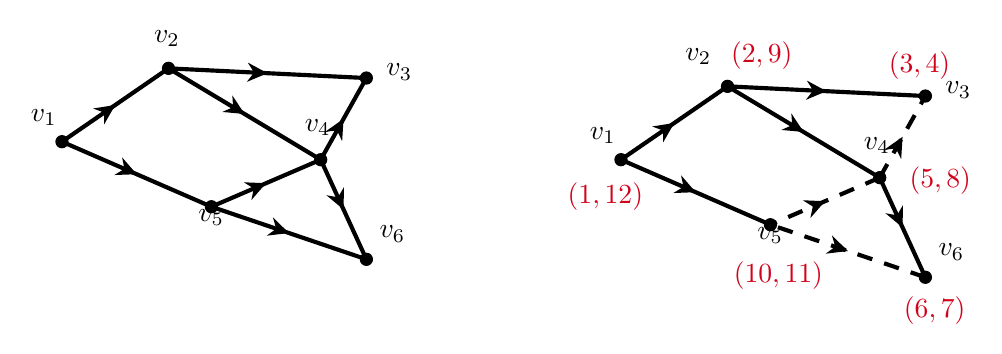
\begin{tikzpicture}[x=0.5pt,y=0.5pt,yscale=-1,xscale=1]
%uncomment if require: \path (0,279); %set diagram left start at 0, and has height of 279

%Flowchart: Connector [id:dp25768028354089545] 
\draw  [fill={rgb, 255:red, 0; green, 0; blue, 0 }  ,fill opacity=1 ] (182,184) .. controls (182,181.58) and (183.96,179.62) .. (186.38,179.62) .. controls (188.79,179.62) and (190.75,181.58) .. (190.75,184) .. controls (190.75,186.42) and (188.79,188.38) .. (186.38,188.38) .. controls (183.96,188.38) and (182,186.42) .. (182,184) -- cycle ;
%Straight Lines [id:da3213985389932459] 
\draw [color={rgb, 255:red, 0; green, 0; blue, 0 }  ,draw opacity=1 ][line width=1.5]    (265.38,150) -- (186.38,184) ;
\draw [shift={(225.88,167)}, rotate = 156.71] [fill={rgb, 255:red, 0; green, 0; blue, 0 }  ,fill opacity=1 ][line width=0.08]  [draw opacity=0] (14.56,-6.99) -- (0,0) -- (14.56,6.99) -- (9.67,0) -- cycle    ;
%Straight Lines [id:da9613590638987879] 
\draw [color={rgb, 255:red, 0; green, 0; blue, 0 }  ,draw opacity=1 ][line width=1.5]    (265.38,150) -- (298.38,91) ;
\draw [shift={(281.88,120.5)}, rotate = 479.22] [fill={rgb, 255:red, 0; green, 0; blue, 0 }  ,fill opacity=1 ][line width=0.08]  [draw opacity=0] (14.56,-6.99) -- (0,0) -- (14.56,6.99) -- (9.67,0) -- cycle    ;
%Flowchart: Connector [id:dp35549046000073203] 
\draw  [fill={rgb, 255:red, 0; green, 0; blue, 0 }  ,fill opacity=1 ] (151,84) .. controls (151,81.58) and (152.96,79.62) .. (155.38,79.62) .. controls (157.79,79.62) and (159.75,81.58) .. (159.75,84) .. controls (159.75,86.42) and (157.79,88.38) .. (155.38,88.38) .. controls (152.96,88.38) and (151,86.42) .. (151,84) -- cycle ;
%Flowchart: Connector [id:dp15983595848302] 
\draw  [fill={rgb, 255:red, 0; green, 0; blue, 0 }  ,fill opacity=1 ] (74,137) .. controls (74,134.58) and (75.96,132.62) .. (78.38,132.62) .. controls (80.79,132.62) and (82.75,134.58) .. (82.75,137) .. controls (82.75,139.42) and (80.79,141.38) .. (78.38,141.38) .. controls (75.96,141.38) and (74,139.42) .. (74,137) -- cycle ;
%Straight Lines [id:da9178716945171659] 
\draw [color={rgb, 255:red, 0; green, 0; blue, 0 }  ,draw opacity=1 ][line width=1.5]    (155.38,84) -- (78.38,137) ;
\draw [shift={(116.88,110.5)}, rotate = 145.46] [fill={rgb, 255:red, 0; green, 0; blue, 0 }  ,fill opacity=1 ][line width=0.08]  [draw opacity=0] (14.56,-6.99) -- (0,0) -- (14.56,6.99) -- (9.67,0) -- cycle    ;
%Straight Lines [id:da6927049634852668] 
\draw [color={rgb, 255:red, 0; green, 0; blue, 0 }  ,draw opacity=1 ][line width=1.5]    (78.38,137) -- (186.38,184) ;
\draw [shift={(132.38,160.5)}, rotate = 203.52] [fill={rgb, 255:red, 0; green, 0; blue, 0 }  ,fill opacity=1 ][line width=0.08]  [draw opacity=0] (14.56,-6.99) -- (0,0) -- (14.56,6.99) -- (9.67,0) -- cycle    ;
%Flowchart: Connector [id:dp4883587595514417] 
\draw  [fill={rgb, 255:red, 0; green, 0; blue, 0 }  ,fill opacity=1 ] (294,91) .. controls (294,88.58) and (295.96,86.62) .. (298.38,86.62) .. controls (300.79,86.62) and (302.75,88.58) .. (302.75,91) .. controls (302.75,93.42) and (300.79,95.38) .. (298.38,95.38) .. controls (295.96,95.38) and (294,93.42) .. (294,91) -- cycle ;
%Straight Lines [id:da8770282704000738] 
\draw [color={rgb, 255:red, 0; green, 0; blue, 0 }  ,draw opacity=1 ][line width=1.5]    (265.38,150) -- (155.38,84) ;
\draw [shift={(210.38,117)}, rotate = 210.96] [fill={rgb, 255:red, 0; green, 0; blue, 0 }  ,fill opacity=1 ][line width=0.08]  [draw opacity=0] (14.56,-6.99) -- (0,0) -- (14.56,6.99) -- (9.67,0) -- cycle    ;
%Flowchart: Connector [id:dp44814914544288187] 
\draw  [fill={rgb, 255:red, 0; green, 0; blue, 0 }  ,fill opacity=1 ] (261,150) .. controls (261,147.58) and (262.96,145.62) .. (265.38,145.62) .. controls (267.79,145.62) and (269.75,147.58) .. (269.75,150) .. controls (269.75,152.42) and (267.79,154.38) .. (265.38,154.38) .. controls (262.96,154.38) and (261,152.42) .. (261,150) -- cycle ;
%Straight Lines [id:da7541359317150998] 
\draw [color={rgb, 255:red, 0; green, 0; blue, 0 }  ,draw opacity=1 ][line width=1.5]    (155.38,84) -- (298.38,91) ;
\draw [shift={(226.88,87.5)}, rotate = 182.8] [fill={rgb, 255:red, 0; green, 0; blue, 0 }  ,fill opacity=1 ][line width=0.08]  [draw opacity=0] (14.56,-6.99) -- (0,0) -- (14.56,6.99) -- (9.67,0) -- cycle    ;
%Flowchart: Connector [id:dp46828077657341205] 
\draw  [fill={rgb, 255:red, 0; green, 0; blue, 0 }  ,fill opacity=1 ] (294,222) .. controls (294,219.58) and (295.96,217.62) .. (298.38,217.62) .. controls (300.79,217.62) and (302.75,219.58) .. (302.75,222) .. controls (302.75,224.42) and (300.79,226.38) .. (298.38,226.38) .. controls (295.96,226.38) and (294,224.42) .. (294,222) -- cycle ;
%Straight Lines [id:da35084682284501567] 
\draw [color={rgb, 255:red, 0; green, 0; blue, 0 }  ,draw opacity=1 ][line width=1.5]    (298.38,222) -- (265.38,150) ;
\draw [shift={(281.88,186)}, rotate = 245.38] [fill={rgb, 255:red, 0; green, 0; blue, 0 }  ,fill opacity=1 ][line width=0.08]  [draw opacity=0] (14.56,-6.99) -- (0,0) -- (14.56,6.99) -- (9.67,0) -- cycle    ;
%Straight Lines [id:da7192255507664823] 
\draw [color={rgb, 255:red, 0; green, 0; blue, 0 }  ,draw opacity=1 ][line width=1.5]    (298.38,222) -- (186.38,184) ;
\draw [shift={(242.38,203)}, rotate = 198.74] [fill={rgb, 255:red, 0; green, 0; blue, 0 }  ,fill opacity=1 ][line width=0.08]  [draw opacity=0] (14.56,-6.99) -- (0,0) -- (14.56,6.99) -- (9.67,0) -- cycle    ;
%Flowchart: Connector [id:dp5254822759541935] 
\draw  [fill={rgb, 255:red, 0; green, 0; blue, 0 }  ,fill opacity=1 ] (586,197) .. controls (586,194.58) and (587.96,192.62) .. (590.38,192.62) .. controls (592.79,192.62) and (594.75,194.58) .. (594.75,197) .. controls (594.75,199.42) and (592.79,201.38) .. (590.38,201.38) .. controls (587.96,201.38) and (586,199.42) .. (586,197) -- cycle ;
%Straight Lines [id:da1169419009661199] 
\draw [color={rgb, 255:red, 0; green, 0; blue, 0 }  ,draw opacity=1 ][line width=1.5]  [dash pattern={on 5.63pt off 4.5pt}]  (669.38,163) -- (590.38,197) ;
\draw [shift={(629.88,180)}, rotate = 156.71] [fill={rgb, 255:red, 0; green, 0; blue, 0 }  ,fill opacity=1 ][line width=0.08]  [draw opacity=0] (14.56,-6.99) -- (0,0) -- (14.56,6.99) -- (9.67,0) -- cycle    ;
%Straight Lines [id:da26586532949811814] 
\draw [color={rgb, 255:red, 0; green, 0; blue, 0 }  ,draw opacity=1 ][line width=1.5]  [dash pattern={on 5.63pt off 4.5pt}]  (669.38,163) -- (702.38,104) ;
\draw [shift={(685.88,133.5)}, rotate = 479.22] [fill={rgb, 255:red, 0; green, 0; blue, 0 }  ,fill opacity=1 ][line width=0.08]  [draw opacity=0] (14.56,-6.99) -- (0,0) -- (14.56,6.99) -- (9.67,0) -- cycle    ;
%Flowchart: Connector [id:dp15507914052855587] 
\draw  [fill={rgb, 255:red, 0; green, 0; blue, 0 }  ,fill opacity=1 ] (555,97) .. controls (555,94.58) and (556.96,92.62) .. (559.38,92.62) .. controls (561.79,92.62) and (563.75,94.58) .. (563.75,97) .. controls (563.75,99.42) and (561.79,101.38) .. (559.38,101.38) .. controls (556.96,101.38) and (555,99.42) .. (555,97) -- cycle ;
%Flowchart: Connector [id:dp6601022829121554] 
\draw  [fill={rgb, 255:red, 0; green, 0; blue, 0 }  ,fill opacity=1 ] (478,150) .. controls (478,147.58) and (479.96,145.62) .. (482.38,145.62) .. controls (484.79,145.62) and (486.75,147.58) .. (486.75,150) .. controls (486.75,152.42) and (484.79,154.38) .. (482.38,154.38) .. controls (479.96,154.38) and (478,152.42) .. (478,150) -- cycle ;
%Straight Lines [id:da41593625130370826] 
\draw [color={rgb, 255:red, 0; green, 0; blue, 0 }  ,draw opacity=1 ][line width=1.5]    (559.38,97) -- (482.38,150) ;
\draw [shift={(520.88,123.5)}, rotate = 145.46] [fill={rgb, 255:red, 0; green, 0; blue, 0 }  ,fill opacity=1 ][line width=0.08]  [draw opacity=0] (14.56,-6.99) -- (0,0) -- (14.56,6.99) -- (9.67,0) -- cycle    ;
%Straight Lines [id:da11185389810538449] 
\draw [color={rgb, 255:red, 0; green, 0; blue, 0 }  ,draw opacity=1 ][line width=1.5]    (482.38,150) -- (590.38,197) ;
\draw [shift={(536.38,173.5)}, rotate = 203.52] [fill={rgb, 255:red, 0; green, 0; blue, 0 }  ,fill opacity=1 ][line width=0.08]  [draw opacity=0] (14.56,-6.99) -- (0,0) -- (14.56,6.99) -- (9.67,0) -- cycle    ;
%Flowchart: Connector [id:dp7957077006041346] 
\draw  [fill={rgb, 255:red, 0; green, 0; blue, 0 }  ,fill opacity=1 ] (698,104) .. controls (698,101.58) and (699.96,99.62) .. (702.38,99.62) .. controls (704.79,99.62) and (706.75,101.58) .. (706.75,104) .. controls (706.75,106.42) and (704.79,108.38) .. (702.38,108.38) .. controls (699.96,108.38) and (698,106.42) .. (698,104) -- cycle ;
%Straight Lines [id:da40385762087990074] 
\draw [color={rgb, 255:red, 0; green, 0; blue, 0 }  ,draw opacity=1 ][line width=1.5]    (669.38,163) -- (559.38,97) ;
\draw [shift={(614.38,130)}, rotate = 210.96] [fill={rgb, 255:red, 0; green, 0; blue, 0 }  ,fill opacity=1 ][line width=0.08]  [draw opacity=0] (14.56,-6.99) -- (0,0) -- (14.56,6.99) -- (9.67,0) -- cycle    ;
%Flowchart: Connector [id:dp6299143679283729] 
\draw  [fill={rgb, 255:red, 0; green, 0; blue, 0 }  ,fill opacity=1 ] (665,163) .. controls (665,160.58) and (666.96,158.62) .. (669.38,158.62) .. controls (671.79,158.62) and (673.75,160.58) .. (673.75,163) .. controls (673.75,165.42) and (671.79,167.38) .. (669.38,167.38) .. controls (666.96,167.38) and (665,165.42) .. (665,163) -- cycle ;
%Straight Lines [id:da6051951368858624] 
\draw [color={rgb, 255:red, 0; green, 0; blue, 0 }  ,draw opacity=1 ][line width=1.5]    (559.38,97) -- (702.38,104) ;
\draw [shift={(630.88,100.5)}, rotate = 182.8] [fill={rgb, 255:red, 0; green, 0; blue, 0 }  ,fill opacity=1 ][line width=0.08]  [draw opacity=0] (14.56,-6.99) -- (0,0) -- (14.56,6.99) -- (9.67,0) -- cycle    ;
%Flowchart: Connector [id:dp9123982617133112] 
\draw  [fill={rgb, 255:red, 0; green, 0; blue, 0 }  ,fill opacity=1 ] (698,235) .. controls (698,232.58) and (699.96,230.62) .. (702.38,230.62) .. controls (704.79,230.62) and (706.75,232.58) .. (706.75,235) .. controls (706.75,237.42) and (704.79,239.38) .. (702.38,239.38) .. controls (699.96,239.38) and (698,237.42) .. (698,235) -- cycle ;
%Straight Lines [id:da09572001479409431] 
\draw [color={rgb, 255:red, 0; green, 0; blue, 0 }  ,draw opacity=1 ][line width=1.5]    (702.38,235) -- (669.38,163) ;
\draw [shift={(685.88,199)}, rotate = 245.38] [fill={rgb, 255:red, 0; green, 0; blue, 0 }  ,fill opacity=1 ][line width=0.08]  [draw opacity=0] (14.56,-6.99) -- (0,0) -- (14.56,6.99) -- (9.67,0) -- cycle    ;
%Straight Lines [id:da9600294712587982] 
\draw [color={rgb, 255:red, 0; green, 0; blue, 0 }  ,draw opacity=1 ][line width=1.5]  [dash pattern={on 5.63pt off 4.5pt}]  (702.38,235) -- (590.38,197) ;
\draw [shift={(646.38,216)}, rotate = 198.74] [fill={rgb, 255:red, 0; green, 0; blue, 0 }  ,fill opacity=1 ][line width=0.08]  [draw opacity=0] (14.56,-6.99) -- (0,0) -- (14.56,6.99) -- (9.67,0) -- cycle    ;

% Text Node
\draw (54,112) node [anchor=north west][inner sep=0.75pt]   [align=left] {$\displaystyle v_{1}$};
% Text Node
\draw (306,196) node [anchor=north west][inner sep=0.75pt]   [align=left] {$\displaystyle v_{6}$};
% Text Node
\draw (175,184) node [anchor=north west][inner sep=0.75pt]   [align=left] {$\displaystyle v_{5}$};
% Text Node
\draw (252,119) node [anchor=north west][inner sep=0.75pt]   [align=left] {$\displaystyle v_{4}$};
% Text Node
\draw (311,79) node [anchor=north west][inner sep=0.75pt]   [align=left] {$\displaystyle v_{3}$};
% Text Node
\draw (143,55) node [anchor=north west][inner sep=0.75pt]   [align=left] {$\displaystyle v_{2}$};
% Text Node
\draw (458,125) node [anchor=north west][inner sep=0.75pt]   [align=left] {$\displaystyle v_{1}$};
% Text Node
\draw (710,209) node [anchor=north west][inner sep=0.75pt]   [align=left] {$\displaystyle v_{6}$};
% Text Node
\draw (579,197) node [anchor=north west][inner sep=0.75pt]   [align=left] {$\displaystyle v_{5}$};
% Text Node
\draw (656,132) node [anchor=north west][inner sep=0.75pt]   [align=left] {$\displaystyle v_{4}$};
% Text Node
\draw (715,92) node [anchor=north west][inner sep=0.75pt]   [align=left] {$\displaystyle v_{3}$};
% Text Node
\draw (527,68) node [anchor=north west][inner sep=0.75pt]   [align=left] {$\displaystyle v_{2}$};
% Text Node
\draw (442,165) node [anchor=north west][inner sep=0.75pt]   [align=left] {$\displaystyle \textcolor[rgb]{0.82,0.01,0.11}{(}\textcolor[rgb]{0.82,0.01,0.11}{1,12}\textcolor[rgb]{0.82,0.01,0.11}{)}$};
% Text Node
\draw (562,222) node [anchor=north west][inner sep=0.75pt]   [align=left] {$\displaystyle \textcolor[rgb]{0.82,0.01,0.11}{(}\textcolor[rgb]{0.82,0.01,0.11}{10,11}\textcolor[rgb]{0.82,0.01,0.11}{)}$};
% Text Node
\draw (685,247) node [anchor=north west][inner sep=0.75pt]   [align=left] {$\displaystyle \textcolor[rgb]{0.82,0.01,0.11}{(}\textcolor[rgb]{0.82,0.01,0.11}{6,7}\textcolor[rgb]{0.82,0.01,0.11}{)}$};
% Text Node
\draw (689,153) node [anchor=north west][inner sep=0.75pt]   [align=left] {$\displaystyle \textcolor[rgb]{0.82,0.01,0.11}{(}\textcolor[rgb]{0.82,0.01,0.11}{5,8}\textcolor[rgb]{0.82,0.01,0.11}{)}$};
% Text Node
\draw (674,70) node [anchor=north west][inner sep=0.75pt]   [align=left] {$\displaystyle \textcolor[rgb]{0.82,0.01,0.11}{(}\textcolor[rgb]{0.82,0.01,0.11}{3,4}\textcolor[rgb]{0.82,0.01,0.11}{)}$};
% Text Node
\draw (560,63) node [anchor=north west][inner sep=0.75pt]   [align=left] {$\displaystyle \textcolor[rgb]{0.82,0.01,0.11}{(}\textcolor[rgb]{0.82,0.01,0.11}{2,9}\textcolor[rgb]{0.82,0.01,0.11}{)}$};


\end{tikzpicture}

}
\caption{Example of running DFS~(with timing) on a DAG $G$. The $[pre,post]$ interval for each vertex
is marked next to each vertex. The $postlist$ for this run is $(v_1, v_5, v_2, v_4, v_6, v_3)$, which is a linearization of $G$.}
\end{figure}


